\documentclass[a4paper]{report}

\usepackage[utf8]{inputenc}
\usepackage[english]{babel}
\usepackage[T1]{fontenc}

\usepackage{geometry}
\usepackage{amssymb}
\usepackage{amsmath}
\usepackage{ifthen}
\usepackage{caption}
\usepackage{graphicx}
\usepackage{subcaption}
\usepackage{minted}
\usepackage{siunitx}
\usepackage[version=4]{mhchem}
\usepackage[dvipsnames]{xcolor}
\usepackage[ED=MEGEP-DyF, Ets=ISAE]{tlsflyleaf/tlsflyleaf}
\usepackage{array}
\usepackage{tcolorbox}


\renewcommand*{\vec}[1]{\underline{#1}}
\newcommand*{\mat}[1]{\vec{\vec{#1}}}
\newcommand{\norm}[2][]{\left\|{#2}\right\|\ifthenelse{\equal{#1}{}}{}{_{{#1}}}}
\newcommand{\RKBar}{\rule[-1.1ex]{0pt}{0pt} \\ \hline \rule{0pt}{2.6ex} &}
\newcommand{\transpose}[1]{{#1}^T}
\newcommand{\krylov}[2][]{\ifthenelse{\equal{#1}{}}{\mathcal{K}_{#2}}{\mathcal{K}_{#2}\left({#1}\right)}}

\newcolumntype{M}[1]{>{\centering\arraybackslash}m{#1}}

\usepackage[pdfpagelabels]{hyperref}
% \hypersetup{
%     colorlinks,
%     linkcolor=black,
%     citecolor=black,
%     % filecolor=black,
%     % urlcolor=black
% }

\newcommand{\GP}[1]{\textbf{\color{BurntOrange}{#1}}}
\newcommand{\LM}[1]{\textbf{\color{ForestGreen}{#1}}}
\newcommand{\PS}[1]{\textbf{\color{Red}{#1}}}
\renewcommand{\GP}[1]{}
\renewcommand{\LM}[1]{}
\renewcommand{\PS}[1]{}


\title{\textbf{\large Méthodologies permettant l'obtention efficace de solutions multi-physiques stationnaires pour des applications en énergétique}}
\author{Pierre Seize}
\defencedate{TBD}
\lab{Office National d'Études et de Recherches Aérospatiales - Département Multi-Physique pour l'Énergétique}
% \\ OU \\ ISAE-ONERA EDyF Energétique et Dynamique des Fluides}
\njudge{7}
\nboss{2}
\nreferee{2}
\makesomeone{judge}{1}{Jocelyne ERHEL}{Directrice de recherche}{Membre du jury}
\makesomeone{judge}{2}{Pierre-Henri MAIRE}{Directeur de recherche}{Membre du jury}
\makesomeone{judge}{3}{Xavier VASSEUR}{Docteur, HDR}{Membre du jury}
\makesomeone{judge}{4}{Rodolphe TURPAULT}{Professeur des Universités}{Rapporteur}
\makesomeone{judge}{5}{Vincent PERRIER}{Chargé de recherche, HDR}{Rapporteur}
\makesomeone{judge}{6}{Guillaume PUIGT}{Directeur de recherche}{Directeur de thèse}
\makesomeone{judge}{7}{Lionel MATUSZEWSKI}{Docteur}{Co-Directeur de thèse}
\makesomeone{referee}{1}{Rodolphe TURPAULT}{Professeur des Universités}{}
\makesomeone{referee}{2}{Vincent PERRIER}{Chargé de recherche}{}
\makesomeone{boss}{1}{Guillaume PUIGT}{}{}
\makesomeone{boss}{2}{Lionel MATUSZEWSKI}{}{}


\begin{document}

\pagenumbering{Alph}
\makeflyleaf
\pagenumbering{arabic}

\tableofcontents
\addcontentsline{toc}{chapter}{Table of contents}

\chapter*{Introduction}
\addcontentsline{toc}{chapter}{Introduction}


  \section*{Contexte}

    \paragraph{}
    Ce travail s'ancre dans le domaine de la simulation numérique de la dynamique des fluides, appliquée à l'énergétique.
    Ce domaine regroupe de nombreux acteurs industriels (Ariane group, DGA, Safran, Airbus, ...) ainsi qu'académiques (ONERA, CERFACS, DLR, universités, ...).
    Il s'intéresse à la manière de simuler avec un calculateur un écoulement fluide en essayant de représenter fidèlement la réalité physique.
    Les différents acteurs de ce domaine ont besoin de pouvoir accéder à certaines grandeurs physiques associées à des phénomènes et à des régimes de fonctionnement bien particuliers.
    Il arrive souvent que ces régimes ne soient pas réalisables à notre échelle, en raison de limitations matérielles ou financières.
    On peut prendre comme exemple l’étude du givrage qui a lieu sur la voilure d’un avion, qui est réalisable expérimentalement mais représente un budget imposant pour l’avionneur, ou bien l’étude des transferts thermiques d’une capsule de rentrée atmosphérique, bien plus difficile à réaliser expérimentalement.
    Pour contourner ces limitations, la simulation numérique est la meilleure option, car elle permet de modéliser un tel cas d’étude par l’exécution d’un programme informatique, et d’obtenir un ensemble important de données qui seront analysées par la suite pour répondre aux questions souhaitées.
    L'analyse de la physique produit en général un ensemble d'équations, souvent des équations aux dérivées partielles, représentant le système réel que l'on souhaite étudier.
    Des algorithmes sont alors nécessaires pour déterminer l'écoulement fluide à partir de ces équations, dans le domaine de travail, en fonction du temps.
    Ainsi, pour obtenir les grandeurs souhaitées, le système physique est intégré temporellement à l'aide d'algorithmes mathématiques afin d'obtenir son évolution dans le temps.
    Souvent, le résultat attendu n'est pas l'évolution temporelle complète du système, mais seulement l'obtention de son état d'équilibre.
    On parle alors de simulation stationnaire, en opposition aux simulations instationnaires, qui cherchent à décrire correctement l'évolution temporelle du système.

    \paragraph{}
    Pour l'ensemble de ces acteurs, l'enjeu le plus crucial est de parvenir à obtenir un bon compromis entre temps de calcul et fidélité du résultat.
    En effet, un calcul rapide à tendance à être peu fidèle à la physique, alors qu'un calcul fidèle tend à utiliser plus de ressources informatiques que celles à disposition.
    Pour un calcul stationnaire, la rapidité correspond au fait d'obtenir la solution \emph{convergée} à un faible coût de calcul et humain.
    Cela ce traduit alors par un compromis entre une simulation très coûteuse en ressources informatiques, prenant un temps long, et qui donne des résultats précis et proches de la physique, et une simulation rapide, économe en ressources, mais pour laquelle les résultats ne sont pas significatifs.
    La nécessité de ce compromis vient du fait des algorithmes utilisés dans ces simulations, ainsi que des paramètres donnés à ces algorithmes.
    Une personne développant un outil de simulation numérique doit donc choisir les algorithmes à utiliser pour obtenir un compromis qu'il estime satisfaisant.
    L'intérêt final pour un acteur dans la simulation numérique de la dynamique des fluides est donc d'avoir un résultat suffisamment précis et suffisamment peu cher à obtenir.
    Un résultat précis est nécessaire pour répondre aux questions qui ont nécessité la simulation.
    La recherche d'un résultat peu cher à obtenir est motivée par des questions d'économies en coût de calcul.
    Ce coût englobe le coût en temps de la simulation, payé par l'utilisateur (et indirectement par l'employeur au travers du salaire) et le coût en ressources informatiques payé par l'employeur, c'est à dire en électricité et en investissement dans des machines plus performantes.

    \paragraph{}
    En fonction du problème que l'on souhaite résoudre, il existe des algorithmes et des méthodes plus ou moins adaptées.
    Dans le cas des problèmes d'énergétique et de multi-physique, les méthodes issues de l'aérodynamique plus traditionnelle sont limitées par le couplage entre les différentes physiques qui possèdent leurs temps caractéristiques distincts.
    Ainsi, les algorithmes utilisés pour la simulation numérique de la dynamique des fluides classique, c'est à dire concentrée sur la résolution des équations de Navier--Stokes, ne sont pas forcément les plus adaptés à une simulation dans le domaine de l'énergétique.
    La mise en jeu plusieurs phénomènes physiques distincts impose en effet des contraintes sur le choix et l'utilisation des algorithmes.
    En conséquence, il serait bon d'adapter ou de remplacer les algorithmes intervenant dans l'intégration temporelle pour les problèmes multi-physiques.


  \section*{Études}

    \paragraph{}
    Si la simulation numérique s'est grandement développée dans le domaine l'aéronautique, elle ne s'est pas tant adaptée au domaine de la multi-physique, et de nombreux codes industriels se contentent de réutiliser les mêmes algorithmes.
    C'est l'exemple du code CEDRE, développé à l'ONERA par le Département Multi-Physique pour l'Énergétique.
    Ce code constitue une plateforme regroupant plusieurs solveurs pour intégrer plusieurs physiques : chaque solveur est dédié à son modèle physique.
    On compte alors un solveur pour la résolution des écoulements compressibles, multi-fluides, réactifs et turbulents, deux solveurs pour le calcul de phase dispersée (gouttes, cristaux, particules) en approche eulérienne et lagrangienne respectivement, un solveur dédié au calcul des films liquides, un solveur dédié au rayonnement, ...
    Des travaux on été fais pour mettre en place une intégration temporelle adaptée aux problèmes résolus par CEDRE.
    C'est par exemple le cas de \cite{Selva1998}.
    Un travail sur l'intégration temporelle a mené au développement de méthodes d'intégrations implicites pour l'intégration des problèmes stationnaires, et au développement d'une méthode GMRES pour la résolution des systèmes linéaires.
    Ainsi, CEDRE constitue en fait un solveur global adapté aux problèmes multi-physiques.
    L'utilisateur peut choisir parmi un panel de méthodes d'intégrations pour obtenir une méthode adaptée à son problème.
    Cependant, la couplage faible entre solveurs entache la convergence vers l'état stationnaire et le choix dans les méthodes d'intégration est limité, en comparaison à ce qu'on peut trouver dans la littérature.
    C'est du moins l'avis des acteurs du code CEDRE, c'est à dire ses développeurs et ses utilisateurs, qui aimeraient des méthodes plus robustes pour pouvoir utiliser CEDRE sur des problèmes plus raides, et convergeant plus vite pour économiser en coût de calcul.

    \paragraph{}\PS{TODO}
    Du coté de la recherche, cependant, de nombreux efforts ont été réalisés dans le sens de la multi-physique, mais ne sont pas encore sorti du cadre académique.
    C'est par exemple le cas de \cite{WongKwokHorneEtAl2019}, qui se sont intéressés à l'intégration temporelle d'équations couplées.
    Ils ont conçu une méthode d'intégration adaptée aux équations couplées, qui est une évolution d'une méthode du point fixe avec en plus une étape d'une méthode de Newton.
    Ils ont ensuite comparés cette méthode à la méthode du point fixe standard, plus généralement utilisée pour une résolution couplée.
    En mettant en place leur méthode sur deux problèmes de couplage simple, ils ont enfin montré l’intérêt de leur méthode par rapport à la méthode de base.
    Si cette méthode se prête bien à leur calculs, elle n'est cependant mise en place que pour des problèmes simples, moins complexes que les problèmes multi-physiques que CEDRE souhaite résoudre.
    De plus, les tests réalisés sont sur des problèmes à l'échelle académique, et non industrielle.

    \paragraph{}
    Parallèlement, des outils utilisés dans le cadre de la simulation aérodynamique pourraient s'avérer intéressants pour des problèmes multi-physiques.
    La méthode JFNK est déjà bien utilisée dans la simulation numérique des équations de Navier-Stokes.
    Dans \cite{ParkNourgalievMartineauEtAl2009}, un mécanisme d'intégration temporelle est mis en place autour d'une formulation JFNK.
    Un préconditionnement basé sur la physique est développé pour résoudre plus précisément le problème linéaire.
    Cette intégration temporelle est ensuite testée sur un problème de cavitée carée thermiquement entrainée.
    Cependant, cette méthode ne s'intéresse seulement aux équations de Navier-Stokes et n'est pas directement appliquable aux problèmes plus généraux de l'énergétique.
    De plus, elle n'est testée que sur un problème académique 2D.

    \PS{TODO: quand parler de la distinction CEDRE / CHARME, placer \cite{ReflochCourbetMurroneEtAl2011}}

  \section*{Bilan général}

    \paragraph{}
    On voit donc que des méthodes numériques sont déjà disponibles pour résoudre des problèmes de simulation numérique.
    En particulier, il existe déjà des solveurs capables de résoudre les problèmes stationnaire multi-physiques d'échelle industrielle.
    D'un autre coté, d'autres méthodes développées dans un cadre académique ont montré leur intérêt sur des problèmes multi-physiques simples.

    Enfin, des méthodes améliorant la résolution des problèmes d'aérodynamique pourraient s'avérer intéressantes pour des problèmes multi-physiques.

    Enfin, certaines méthodes récentes ont permis ...

    Les solveurs déjà existants utilisent des méthodes anciennes, ou peu adaptées aux problèmes multi-physiques.
    Les méthodes plus performantes ne sont utilisées que sur des problèmes simplifiés, ou dans des calculs d'échelle académique.

    Il semblerait maintenant intéressant d'adapter ces nouvelles méthodes pour la résolution des problèmes multi-physiques dans un code industriel.

    \vspace{1cm}\hrule\vspace{1cm}

  \section*{C'est ce qui justifie cette étude ...}

    \paragraph{}
    ..., elle consiste à améliorer la convergence, la rapidité et la robustesse de l'intégration temporelle de la plateforme CEDRE sur les problèmes stationnaires multi-physiques en ajoutant des méthodes numériques non utilisées dans la simulation numérique industrielle.


  \section*{Démarche}

    \paragraph{}
    L'objectif du chapitre 1 a été de développer une formulation JFNK pour AMÉLIORER QUOI DE l'intégration temporelle dans le code CEDRE.
    JUSTIFICATION
    Pour cela, l'idée a été d'adapter la méthode d'intégration en s'inspirant de la bibliographie en fonction de certains critères.
    L'idée suivante a été de développer une méthode de Newton afin de résoudre le problème non linéaire sachant que celui ci est produit par les méthodes d'intégration implicites utilisées lors de la résolution des problèmes stationnaires.
    L'idée suivante a été de développer une formulation sans matrice du système afin de mieux former les systèmes linéaires et permettre un couplage fort des solveurs de CEDRE.
    L'idée suivante a été d'adapter la résolution du système linéaire en utilisant des méthodes plus modernes que la méthode actuelle, en s'inspirant de la bibliographie, afin de résoudre plus précisément le système linéaire.
    On a alors obtenu une méthodologie d'intégration temporelle utilisable pour résoudre des problèmes multi-physique stationaires.
    A ce stade, cette méthode fonctionne au sens où elle permet d'obtenir un résultat à un problème de simulation numérique, mais elle n'est pas encore caractérisée.

    \paragraph{}
    L'idée du chapitre 2 a été d'évaluer la robustesse et la convergence de la formulation JFNK sur des problèmes stationnaire en multi-physiques au sein du code CEDRE.
    Pour cela, l'idée a été de sélectionner des cas tests de complexité croissante afin de représenter un ensemble de problèmes multi-physiques.
    L'idée suivante a été de mettre en place une méthode d'évaluation des performances de l'intégration temporelle afin de caractériser sa robustesse et sa vitesse de convergence.
    L'idée suivante a été de montrer que sur ces cas la formulation améliore la robustesse et la convergence afin de valider la pertinance du choix de la méthode.
    On estime qu'on a alors développé une méthode d'intégration temporelle "efficace", c'est à dire rendant l'intégration temporelle de CEDRE plus robuste et convergeant plus rapidement sur un ensemble de problèmes multi-physiques.
    On pourrait aller plus loin mais on va plutôt regarder l'intérêt de la formulation JFNK sur des problèmes autres pouvant en tirer profit : les problèmes instationnaires à grand pas de temps.

    \paragraph{}
    L'idée du chapitre 3 est d'analyser la formulation JFNK sur les problèmes instationnaires à grand pas de temps.
    Pour cela, l'idée a été d'identifier une classe de problèmes sortant du cadre initial de la thèse mais pouvant bénéficier de la formulation JFNK, afin d'y démontrer l'intérêt de la formulation.
    L'idée suivante a été de concevoir un cas d'étude afin de de mettre en valeur l'intérêt de la formulation JFNK.
    L'idée suivante a été de montrer l’intérêt la formulation sur ce cas.


\section*{TODO}
\begin{itemize}
  \item Conclusion chapitre 3
  \item Conclusion chapitre 4
  \item Conclusion chapitre 5
  \item Parler de l'AID
  \item Conclusion générale
  \item \GP{VIRER LES ESPACES ENTRE UNE EQUATION ET LE POINT}
  \item Pronom we
  \item noms de parties en français
  \item nom de chapitres trop longs qui empietent sur le numéro de page
\end{itemize}


\part{Résolution efficace des problèmes stationnaires en multi-physique}

  \chapter{Analysis of existing methods}

  \section{Problem setup}

    \paragraph{}
    In this part we are going to set the mathematical framework for this study.
    We will start from a partial differential equation arising from the physical model, in the form of
    \begin{equation}\label{eq:pde}
      \frac{\partial \xi}{\partial t} + \operatorname{F}\left(\xi\right) = 0
    \end{equation}
    where the function $\operatorname{F}$ uses some space derivatives of the state variable $\xi$.
    This equation then describe the temporal evolution of the state variables $\xi$.

    \paragraph{}
    A particular class of such partial differential equations are conservative equations.
    They correspond to the case where the function $\operatorname{F}$ can be written as a divergence term.
    Finally, with a source term $\operatorname{S}$, those equations look like:
    \begin{equation}\label{eq:pde_conservative}
      \frac{\partial \xi}{\partial t} + \nabla \cdot \vec{\operatorname{f}}\left(\xi\right) = \operatorname{S}\ .
    \end{equation}
    One might notice that equation (\ref{eq:pde_conservative}) is indeed a particularisation of equation (\ref{eq:pde}), with $\operatorname{F}\left(\xi\right) = \nabla\cdot \vec{\operatorname{f}}\left(\xi\right) - \operatorname{S}$.
    Those conservative equations are the one we will focus on is this study, as they describe the physical systems we are interested in.

    \paragraph{}
    In this work, we will talk about computational fluid dynamics.
    We are in fact mostly interested in the Navier--Stokes equation, and its variants: the reactive Navier--Stokes equation, the Reynold-averaged Navier--Stokes equation, etc.
    A simple form of this equation can be:
    \begin{equation}\label{eq:ns}
      \left\{\begin{aligned}
        &\partial_t\left(\rho         \right) &&+ \nabla\cdot\left( \rho \vec{u} \right) &&= 0 \\
        &\partial_t\left(\rho \vec{u} \right) &&+ \nabla\cdot\left( \rho \vec{u} \otimes \vec{u} + p \id \right) &&= \nabla\cdot \mat{\tau}\\
        &\partial_t\left( \rho E      \right) &&+ \nabla\cdot\left( \left(\rho E + p\right) \vec{u} \right) &&=
          \nabla\cdot\left( \mat{\tau} \cdot \vec{u} \right)
      \end{aligned}\right.
    \end{equation}
    with the \PS{relation de fermeture} $\rho E = \frac{p}{\gamma - 1} + \rho\frac{\vec{u} \cdot \vec{u}}{2}$.
    The deviatoric stress tensor $\tau$ accounts for the viscosity of the fluid, and its computation depends on the model used.
    Without it, one recovers the Euler equations.
    To this simple form can be added source terms from the reactive model, source terms from the turbulence model, divergence terms from a diffusive model, etc.
    Yet it is clear that with a bit of rewriting, we can go back to the starting form (\ref{eq:pde}) and even the conservative form with source terms (\ref{eq:pde_conservative}).
    The quantity $\xi$ is no longer a scalar but a vector with the density $\rho$, each component of the momentum $\rho\vec{u}$ and the energy $\rho E$ as its components.
    Apart from this small change, the idea is the same.

    \paragraph{}
    When solving numerically equations like (\ref{eq:pde}), one must first take a spatial domain on interest.
    Let us call this domain $\mathcal{D}$.
    As we are interested in solving equations numerically, we need to be able to represent different quantities, such as the state variable $\xi$, numerically over the domain $\mathcal{D}$ and store it in the memory of a computer.
    Therefore we need to discretise the continuous spatial domain into a finite number of cells, or elements.
    This is usually done with a mesh of the domain $\mathcal{D}$.
    First we divide the domain $\mathcal{D}$ in a set of cells, called a mesh.
    Those cells are small volumes in 3D, faces in 2D or segments in 1D, disjoints, such as their union recovers the original domain.
    Interest quantities, such as the fluid velocity, density, \dots, are then stored at each nodes, averaged in the center of each cells or sometimes in a more complex fashion depending on the method.
    They are no longer mathematically represented by a function of the continuous physical domain $\xi : \mathcal{D} \rightarrow \mathbb{R}$ but by a finite sized vector $\Xi$ gathering all the information across the discretised domain.
    For some simple discretisation methods, this vector consists of the quantity evaluated at the mesh nodes or averaged at the center of the cells.
    For more complex methods, this vector consists of information used to construct the solution over the domain: polynomial coefficients, spectral decomposition coefficients, etc.
    Anyway, we no longer work in a continuous domain $\mathcal{D}$ but on a discretised one.

    \paragraph{}
    The partial differential equation (\ref{eq:pde}) transforms then into an ordinary differential equation:
    \begin{equation}\label{eq:ode}
      \frac{\partial \Xi}{\partial t} + \operatorname{G}\left(\Xi\right) = 0 \ .
    \end{equation}
    The difference here is that the function $\operatorname{G}$ is a function of a discrete vector whereas $\operatorname{F}$ was a function of a continuous function, and therefore $\operatorname{G}$ does not uses any spatial derivatives.
    Thanks to the spatial discretisation method, the only derivative remaining is with regard to time.
    The rest is then up to the temporal integration method, which is the main topic of this thesis.
    We will work from equation (\ref{eq:ode}) no matter where the function $\operatorname{G}$ comes from, but sometimes understanding the origin of this function can help so we will now introduce the spatial discretisation method used in our solver.


  \section{Brief introduction to the spatial integration schemes}

    \paragraph{}
    A \emph{spatial discretisation method} is the choice of how to represent a quantity over a discretised domain, and how to compute spatial derivative of this quantity from this representation.
    Indeed, before solving equation (\ref{eq:pde}) we need to decide how to transform the continuous model into a discretised one.
    We also have to look at how the spatial derivatives arising from equation (\ref{eq:pde}) translate in the discretised model.

    \subsection{The Finite Volumes method}

      \paragraph{}
      The spatial discretisation method used in the solver CHARME is called the Finite Volumes method \cite{EymardGallouetHerbin2000}.
      This method is particularly well fitted for conservatives equations such as equation (\ref{eq:pde_conservative}).
      Such equation has the property that the quantity $\xi$ is conserved: without source terms, the variation of the total quantity on $\xi$ over the domain $\mathcal{D}$ is equal to the flux $f\left(\xi\right)$ coming through the boundary $\partial\mathcal{D}$.
      In the case of the Navier--Stokes equations (\ref{eq:ns}), the density, the momentum and the energy are conserved throughout time, apart from what comes in and out of the domain.
      In a close domain where nothing comes in or out, they are indeed conserved.
      The main interest of the Finite Volumes method is that this property stays true through the spatial discretisation step.

      \paragraph{}
      The Finite Volumes method consists in integrating the partial differential equation over each cell of the mesh.
      Writing $\mathcal{V}_i$ the volume of the $i$th cell:
      \begin{equation}
        \int_{\mathcal{V}_i} \frac{\partial \xi}{\partial t} \mathrm{d}v + \int_{\mathcal{V}_i} \nabla\cdot \vec{\operatorname{f}}\left(\xi\right) \mathrm{d}v = \int_{\mathcal{V}_i} \operatorname{S} \mathrm{d}v\ .
      \end{equation}
      Then the Green--Ostrogradski theorem transforms the flux divergence into a \PS{bilan surfacique}:
      \begin{equation}
        \frac{\mathrm{d}}{\mathrm{d} t} \int_{\mathcal{V}_i} \xi\mathrm{d}v + \oint_{\partial\mathcal{V}_i} \vec{\operatorname{f}}\left(\xi\right) \cdot \vec{\mathrm{d}s} = \int_{\mathcal{V}_i} \operatorname{S} \mathrm{d}v\ .
      \end{equation}
      By writing $\square_i = \frac{1}{\left\|\mathcal{V}_i\right\|} \int_{\mathcal{V}_i} \square \mathrm{d}v$ the average in the $i$th cell, we then have:
      \begin{equation}
        \frac{\mathrm{d}\xi_i}{\mathrm{d} t}  + \frac{1}{\left\|\mathcal{V}_i\right\|} \oint_{\partial\mathcal{V}_i} \vec{\operatorname{f}}\left(\xi\right) \cdot \vec{\mathrm{d}s} = \operatorname{S}_i \ .
      \end{equation}

      \paragraph{}
      As stated before, the spatial discretisation method do transform the partial differential equation into an ordinary differential equation.
      It tells us to store our quantities as the averaged values represented at the center of gravity of each cells as our vector $\Xi$.
      It also tells us to compute the divergence from equation (\ref{eq:pde_conservative}) as a \PS{bilan surfacique de flux}.
      The last thing to do is to decide how to compute this \PS{bilan surfacique de flux}.
      The cells from our meshes are polygons.
      Therefore they have a finite number of (planar) faces.
      The integral over the boundary of the cell can be decomposed by the faces, to get the approximation:
      \begin{equation}
        \oint_{\partial\mathcal{V}_i} \vec{\operatorname{f}}\left(\xi\right) \cdot \vec{\mathrm{d}s} \approx \sum_{j\textrm{ neighbor of } i} \vec{\operatorname{f}}_{ij} \cdot \vec{s_{ij}}
      \end{equation}
      where $\vec{\operatorname{f}}_{ij} \cdot \vec{s_{ij}}$ is an approximation of the flux going through the face between cells $i$ and $j$.
      This approximation is a key element of the Finite Volumes method, therefore we will discuss it later.
      We can now compute the function $\operatorname{G}$ from equation (\ref{eq:ode}): for each face of the mesh we compute $\vec{\operatorname{f}}_{ij} \cdot \vec{s_{ij}}$, we add this value to the $i$th component and remove it from the $j$th component of our new vector.
      Then, after adding the source terms we get a vector containing the result of $\operatorname{G}\left(\Xi\right)$.
      As can be seen, every contribution of the flux added in a cell is removed from another, and therefore this spatial discretisation method preserves the conservativity of the underlying equation.


    \subsection{The Riemann problem}

      \PS{Déplacer après la reconstruction ? C'est plus fondamental mais ça intervient après}

      \paragraph{}
      The last remaining problem with this presentation of the Finite Volumes method is how to compute the flux going through cell interfaces.
      On the interfaces between two cells we know the left and right quantities $\xi_L$ and $\xi_R$, and we need to compute the corresponging flux.
      It is possible here to use a reconstruction method to get a better approximation of the quantities left and right of the interface, and therefore we end up using the left and right quantities $\xi_L^*$ and $\xi_R^*$.
      The idea is now to compute the flux going through the face as a function of $\xi_L^*$, $\xi_R^*$ and the surface vector $\vec{s}$.
      From the interface point of view, there are two possibly different states, one from each side: this is what is called a Rienamm problem.
      A Riemann problem is an initial value problem applied to a conservation equation, where the initial solution is piecewise constant with a single possible discontinuity.
      By working with the equation and deriving the jump condition, it is possible to compute the quantity at the interface from a possibly discontinuous state at the interface.
      Then it is possible to evaluate the flux associated with this state going through the surface.
      This approach can be called the exact Riemann solver as it uses the exact solution of the Riemann problem.
      But the drawback from this approach usually is the computational coast required to find this exact solution.
      What is usually done is to use approximate Riemann solvers, compromising between speed and accuracy.
      Several Riemann solvers\footnote{\PS{Est-ce qu'on parle toujours de solveur de Riemann (qui trouve la solution du problème idoine) ou on parle de "schéma de flux numérique" ?}} are available to the user in our solver, such as the well known Roe, HLLC or AUSM+ schemes \cite{Roe1981, Toro2009}.





    \subsection{Gradient reconstruction methods}
      \subsubsection{The k-exact method}
      \subsubsection{The Multislope method}


  \section{Time integration methods}
    \subsection{Analyse des méthodes}
      \subsubsection{Consistance et ordre}
      \subsubsection{Stabilité}
    \subsection{Méthodes implicites}
      \subsubsection{Méthode d'Euler implicite}
      \subsubsection{Méthodologie des méthodes implicites}


  \chapter{Development workflow in CEDRE}

  \paragraph{}
  In this chapter we will discuss the details of how we implemented selected methods in CEDRE.
  This does not constitute research work, but it ended up being a large part of the work done during this thesis.
  It is also not without interest, as we used advanced features in order to implement what we set out to do.


  \section{Description of CEDRE}

    \paragraph{}
    The software system CEDRE gather several solvers to solve problems in the field of multiphysics \cite{ReflochCourbetMurroneEtAl2011}.
    Each solver is dedicated to a given model.
    As of today there are seven solvers embedded in CEDRE:
    \begin{itemize}
      \item CHARME, the fluid solver, for compressible multifluid and reactive flow, with RANS or LES turbulence models
      \item SPIREE, the dispersed phase solver using an Eulerian framework
      \item SPARTE, the dispersed phase solver using a Lagrangian framework
      \item ASTRE, the radiation solver using a Monte Carlo method
      \item REA, the radiation solver using a discrete ordinates method
      \item FILM, for shallow water equations used to model ice accretion
      \item ACACIA, the conduction solver, for heat transfer in solids.
    \end{itemize}
    Combining different solvers, CEDRE is able to numerically simulate multiphysic phenomena.
    Using those solvers, CEDRE applications goes from aerodynamics to aeroacoustics, aerothermics, combustion, icing, etc.
    The solver are coupled either through boundary conditions as for example in a thermal interaction at a fluid-structure contact, or inside the computational domain as for example in the case of mass and energy transfer between dispersed phases and the main flow.
    The coupling can either be one-way or two-way, depending on the user's choice.
    Each solver is integrated in time separately, and the coupling consists in some data exchange between iterations: it is an explicit coupling.

    \paragraph{}
    Some functionalities common to multiple solvers exists outside the solver in helper libraries.
    For instance:
    \begin{itemize}
      \item ASSEMBLAGE acts as the conductor by handling the overall simulation, telling the solvers what to do and when to do it, when to exchange data and with which other coupled solver
      \item BIBCEDRE contains tool for geometrical operations, linear algebra methods, mesh handling, parallel communications and other general functionalities
      \item THERMOLIB is used to compute the different thermophysical properties such as heat capacities, chemical reaction rates, etc. \PS{Lionel je dis pas de bêtise sur les coefficients de réaction chimique ?}
    \end{itemize}

    \paragraph{}
    Despite allowing some flexibility in the programming language, most of CEDRE is written in Fortran.
    We decided to keep working with Fortran to help the integration of our work.
    As CEDRE is used by industrial clients, and as they rely on their own supercomputer, we need to limit ourselves to Fortran 2003 standards, so as to ensure compatibility.


  \section{Implementation details}


    \paragraph{}
    In this thesis, we focused on the most used solver: CHARME.
    Indeed, not only is it the most used, but other solvers use it as a base on many applications.
    When simulating ice accretion around a wing profile for example, a standard methodology with CEDRE is to first get the base aerodynamic flow with CHARME, and then compute the ice particles with SPIREE or SPARTE.
    Working with the solver CHARME was the way to benefit the most from our work.
    Even if during this thesis we only worked on CHARME, we always kept in mind that the finality was multiphysics simulations using multiple solvers.
    That is why we tried to develop generic functionalities so that they could be easily imported to other solvers, provided the developers of said solvers wanted to use them.
    The same reason was also used as a criterium in our choices, as was explained previously.
    Choosing the Jacobian Free Newton--Krylov method goes towards fully implicit coupling between solvers, instead of the explicit coupling existing today.

    \subsection{FGMRES}

    \paragraph{}
      In order for our work to be usable in every other solver, we had to work on the common library BIBCEDRE.
      When the implicit Euler method of CHARME needs to solve a linear problem, it uses BIBCEDRE.
      It contains everything needed to solve linear problems, such as GMRES and preconditioners.
      A linear problem is stored in BIBCEDRE as the Fortran derived type \mintinline{fortran}{type_sys}.
      In order to add Flexible proconditioning to the existing GMRES, we added a pointer to an inner instance of \mintinline{fortran}{type_sys} inside of \mintinline{fortran}{type_sys}, so that linear system and its corresponding solver may use an inner solver for an inner problem:
\begin{minted}{fortran}
  type type_sys
    ! Inner linear system and solver
    type(type_sys), pointer :: sys_int => null()

    ... ! Additional data
  end type type_sys
\end{minted}
      This way, when we need to apply the preconditioner during a GMRES iteration, we can use the inner \mintinline{fortran}{type_sys} instance to call the inner GMRES.
      Furthermore, having a pointer to an inner instance allows for more freedom for the inner solver.
      One could for instance use multiple depths of preconditioning and have the inner GMRES also be a FGMRES method, preconditioned by another GMRES, etc.


    \subsection{Matrix free}

      \paragraph{}
      Sparse matrices are stored in an in-house format, using an array for the diagonal blocks, another one for the extra-diagonal blocks and a third one to index the extra-diagonal blocks.
      Matrix vector products are made inside BIBCEDRE to handle this matrix format, with the routine:
\begin{minted}{fortran}
  subroutine gmvec(sys, i_p, i_ap)
    type(type_sys), intent(inout) :: sys
    integer,        intent(in)    :: i_p
    integer,        intent(in)    :: i_ap
\end{minted}
      that takes three arguments: the \mintinline{fortran}{type_sys} instance, an index identifying the vector to multiply and an index identifying the vector where to put the result.
      As we explained when we introduces Krylov subspace methods, GMRES uses the linear system matrix through this matrix vector product routine.
      Classically, a client solver such as CHARME fills the matrix coefficients, and then let BIBCEDRE solve the linear system.
      In order to use the matrix free approximation from equation (\ref{eq:matrix_free}), we only need to replace this routine by a new one that computes the approximation.
      Unfortunately, the approximation uses a function that belongs to the client solver.
      The library BIBCEDRE does not know this function and how to compute it, as it is part of CHARME or any other client solver.
      As we said, we want to write generic solutions, and so merging the library BIBCEDRE with the solver CHARME is not a good solution.
      What we need here is to allow BIBCEDRE to use a callback from the client solver.
      We did that using the Fortran 2003 feature: polymorphism.
      Without going into too much details, we added a member to the type \mintinline{fortran}{type_sys} that contains the context to evaluate a matrix vector product:
\begin{minted}{fortran}
  type type_sys
    ! Matrix vector product context
    class(type_gmvec_ctx), pointer :: gmvec_ctx => null()

    ... ! Additional data
  end type type_sys
\end{minted}
      with:
\begin{minted}{fortran}
  type type_gmvec_ctx
    procedure(interface_gmvec), pointer, nopass :: gmvec

    ... ! Additional data
  end type type_gmvec_ctx
\end{minted}
      This way, when the client solver creates an instance \mintinline{fortran}{sys} of \mintinline{fortran}{type_sys}, it can choose how to evaluate matrix vector products by setting the procedure pointer \mintinline{fortran}{sys%gmvec_ctx%gmvec}.
      It can for example point to the already existing routine to use the classical matrix vector product, but it also can use a custom routine that implements the approximation (\ref{eq:matrix_free}).
      Furthermore, the client solver can use polymorphism and create an extended type of \mintinline{fortran}{type_gmvec_ctx} in order to store additional data into the context.
      This is what is done by the solver CHARME, as it does need additional data to approximate the Jacobian matrix vector product.
      Finally, with this implementation, any solver that wants to use the approximation (\ref{eq:matrix_free}) just needs to write the corresponding routine and set the context accordingly.
      Then, a user can choose at execution time whether to use the standard Jacobian matrix or the matrix free method.


    \subsection{Strategy for the choice of \texorpdfstring{$\varepsilon$}{epsilon}}
      \PS{Bouger cette partie ?}


      \paragraph{}
      When we introduced the approximation (\ref{eq:matrix_free}) we saw a new parameter $\varepsilon$.
      It is easy to check that the truncation error on this approximation decreases linearly with regard to $\varepsilon$.
      It is natural to take a small value for $\varepsilon$.
      But unfortunately, we work with floating-point arithmetic, so dividing by a small $\varepsilon$ introduces roundoff error.
      This parameter needs to balance truncation and roundoff error.
      We need to decide on a strategy for the choice of epsilon.
      We could take for example $\varepsilon = \sqrt{\varepsilon_\textrm{mach}}$ where $\varepsilon_\textrm{mach}$ is the machine epsilon: around $10^{-6}$ for single precision and $10^{-15}$ for double precision.
      This choice is often discarded as it is deemed too simplistic.
      Instead, works from the literature tend to use the same few options \cite{ParkNourgalievMartineauEtAl2009, LiuZhangZhongEtAl2015, AbhyankarBrownConstantinescuEtAl2018} that come from \cite{PerniceWalker1998} and \cite{DennisSchnabel1996}.
      Those options are well described in \cite{KnollKeyes2004}.
      In particular, the one that we encounter the most is the one from \cite{PerniceWalker1998}:
      \begin{equation}\label{eq:epsilon_wp}
        \varepsilon_\textrm{wp} = \frac{\sqrt{\varepsilon_0 \left(1 + \norm[2]{x}\right) }}{\norm[2]{v}}
      \end{equation}
      using the same $x$ and $v$ as in equation (\ref{eq:matrix_free}).
      Here $\varepsilon_0$ is the estimated relative error in function evaluation.
      A reason this choice is so popular is that apart from this $\varepsilon_0$ value, it does not require any user input.
      Furthermore, $\varepsilon_0$ if often simply set to machine epsilon $\varepsilon_\textrm{mach}$.

      \paragraph{}
      To analyse this strategy in the choice of $\varepsilon$, we do the following numerical experiment.
      We consider the 1D Burgers' equation over a regular periodic mesh made of 10 cells (or segments in 1D).
      The function $f$ is taken as the right-hand side of equation (\ref{eq:ode}) when solving the Burgers' equation, using a first-order Finite Volume method as the spatial discretisation method, itself using an exact Riemann solver (Godunov 's scheme).
      This function was chosen because it is a nonlinear conservative equation, often viewed in computational fluid dynamics as a simplified version of Euler equations and it contains most aspects of nonlinear hyperbolic equations.
      The vectors $x$ and $v$ are $10 + r_1$ and $0.1 \left(2 r_2 - 1\right)$ where $r_1$ and $r_2$ are random vectors following a uniform distribution on $\left[0, 1\right[$, obtained with the Python package NumPy: \mintinline{python}{numpy.random.random}.

      \begin{figure}
        \centering
        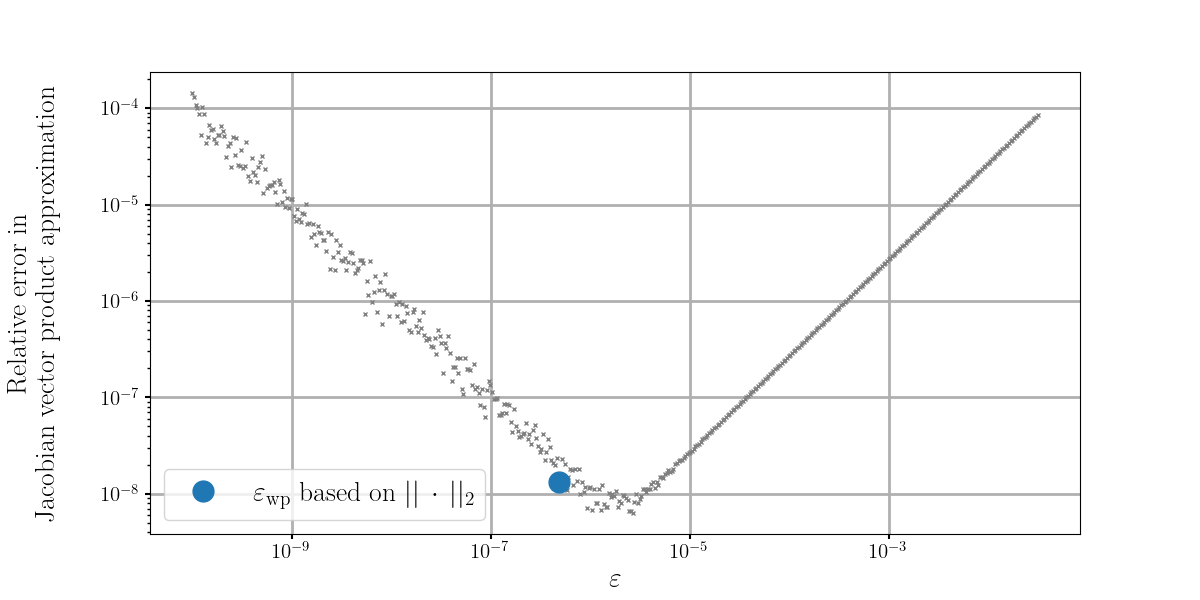
\includegraphics[width=\textwidth]{figures/epsilon_Burgers_10.png}
        \caption{
          Error in the Jacobian matrix vector product approximation as a function of $\varepsilon$, and in particular for the most popular choice $\varepsilon_\textrm{wp}$.
          The function is the right-hand side of equation (\ref{eq:ode}) from a Finite Volume method using an exact Riemann solver for Burgers' equation, over a 10 cell 1D regular mesh.
        }
        \label{fig:epsilon_burgers_10}
      \end{figure}

      \paragraph{}
      The experiment result can be seen on figure \ref{fig:epsilon_burgers_10}.
      The relative error in the approximation is shown as a function of $\varepsilon$ with small gray crosses.
      On the right part of the figure, the error decreases linearly with regard to $\varepsilon$.
      This correspond to a truncation error dominated region.
      On the left part, the error increases as $\varepsilon$ decreases.
      This correspond to a roundoff error dominated region.
      Also, this increase is not smooth as the linear decrease, because roundoff errors tend to produce more chaotic results.
      The choice of $\varepsilon$ from \cite{PerniceWalker1998} is also shown in the figure, as the large blue dot.
      As we can see, it falls into a low error region, not too much on the left, not too much on the right.

      \paragraph{}
      The issue we noticed is the following.
      Some references in the literature do not specify the norm used in equation (\ref{eq:epsilon_wp}).
      As it is most of the time the Euclidian norm $\norm[2]{\,\cdot\,}$, or 2-norm, we can assume that it is also the case when it is not specified.
      However, this means that in our example the value of $\varepsilon_\textrm{wp}$ will depend on the vector size.
      With our example, if we increase the number of cells in our mesh the typical size of the vector components stay roughly the same, so the shape of the error as a function of $\varepsilon$ should not change much from the one in figure \ref{fig:epsilon_burgers_10}.
      But if the vector components size stay the same, the 2-norm does increases with the vector dimension.
      We can even see that when the dimension is $N \gg 1$, $\varepsilon_\textrm{wp} \sim N^{-1/4}$.
      Having $\varepsilon$ to depend on $N$ did not make sense to us, as we are working with possibly large vectors in our industrial applications.
      That is why we decided to use a variation from what is currently found in the literature: we will use the norm $\norm[2]{\,\cdot\,} / \sqrt{N}$ that can be seen as a scaled 2-norm.
      We then get a new strategy for the choice of $\varepsilon$ that we note $\varepsilon_{\textrm{wp}, N}$.

      \begin{figure}
        \centering
        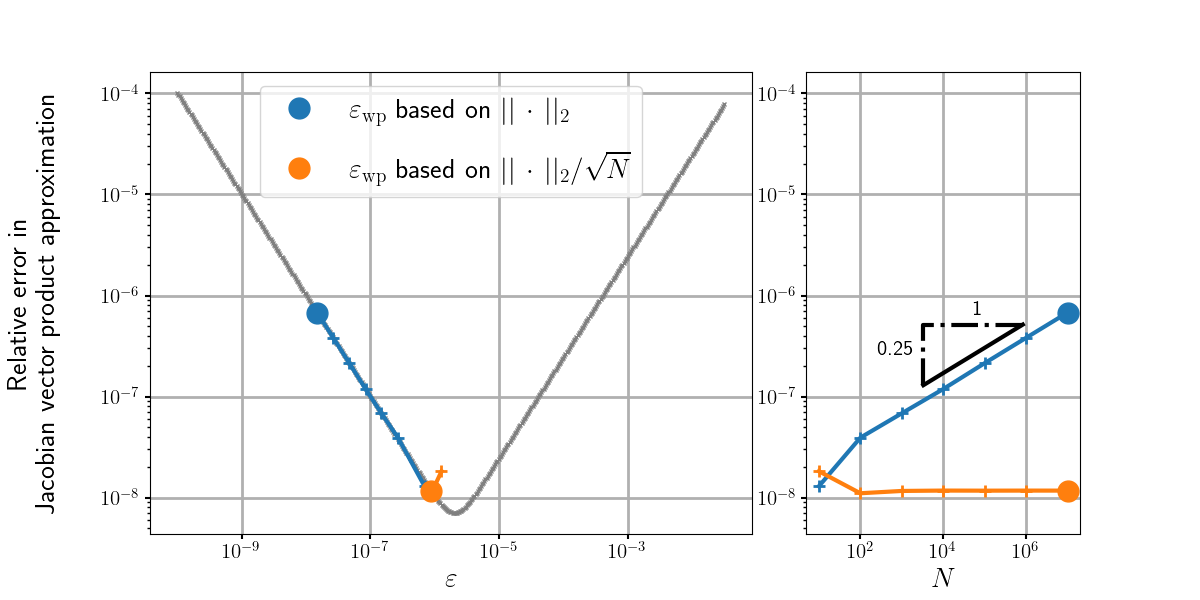
\includegraphics[width=\textwidth]{figures/epsilon_Burgers.png}
        \caption{
          Error in the Jacobian matrix vector product approximation as a function of $\varepsilon$ (left) and of the dimension $N$ (right).
          On the left figure, colored cross markers correspond to the values computed on a mesh of $10^1$, $10^2$, ... cells, and circle markers to the last value with $10^7$ cells.
          Grey cross markers on the left figure correspond to a mesh of $10^7$ cells.
        }
        \label{fig:epsilon_burgers}
      \end{figure}

      \paragraph{}
      We compared the two strategies on the same test case, while increasing the number of cells from 10 to 100, 1000, ..., up to $10^7$.
      Figure \ref{fig:epsilon_burgers} shows the result of this experiment.
      On the left, we see that the shape of the relative error as a function of $\varepsilon$ when $N = 10^7$ is similar to when $N = 10$, albeit the roundoff error dominated region is more regular.
      In particular, the ideal trade off between the two error types did not move a lot.
      We see that as expected, the value or $\varepsilon_\textrm{wp}$ decreases: this translate as the fact that the blue dot moved to the left.
      When looking at the error as a function of the dimension $N$, we can even recover the $-1/4$ expected slope.
      In the right figure we see in fact a $1/4$ slope but the error is inversely proportional to the value of $\varepsilon$ so if the error \PS{varies in} $N^{1/4}$, then $\varepsilon_\textrm{wp}$ \PS{varies in} $N^{-1/4}$.
      Because of the shape of the error as a function of $\varepsilon$, if $\varepsilon_\textrm{wp}$ changes with $N$ it will eventually end up increasing the error.
      This is an undesired feature.
      Our new choice $\varepsilon_{\textrm{wp}, N}$ on the other hand does not change a lot when $N$ increases.
      Therefore, the error level stays the same no matter the dimension.

      \paragraph{}
      The same numerical experiment was made on a more complex case: the 1D Euler equations.
      Here, the function $f$ corresponds to the right-hand side of equation (\ref{eq:ode}) given by a centered Finite Volume method used as the spatial discretisation method, in which the interface flux are defined as an average of left and right fluxes.
      This means the Riemann solver just averages the left and right fluxes.
      This spatial method is known for its instability when used in an actual solver, but it is useful in this experiment as the analytic Jacobian matrix is easy to derive, contrary to methods using more complex Riemann solvers.
      This physical model assigns 3 degrees of freedom in each cell.
      We will use the primitive variables.
      The vector $x$ corresponds to a uniform density of $1\si{\kilogram\per\cubic\meter}$, a velocity equal to a sine making one period over the mesh and of amplitude $10\si{\meter\per\second}$, and uniform pressure of $10^5\si{\pascal}$.
      The vector $v$ is a random vector in $\left[0, 1\right]$ as before, where the first component is scaled by $10^{-3}$, the second by $10^{-2}$, and the third by $10^{2}$, in order to impose $10^{-3}$ relative perturbations.

      \begin{figure}
        \centering
        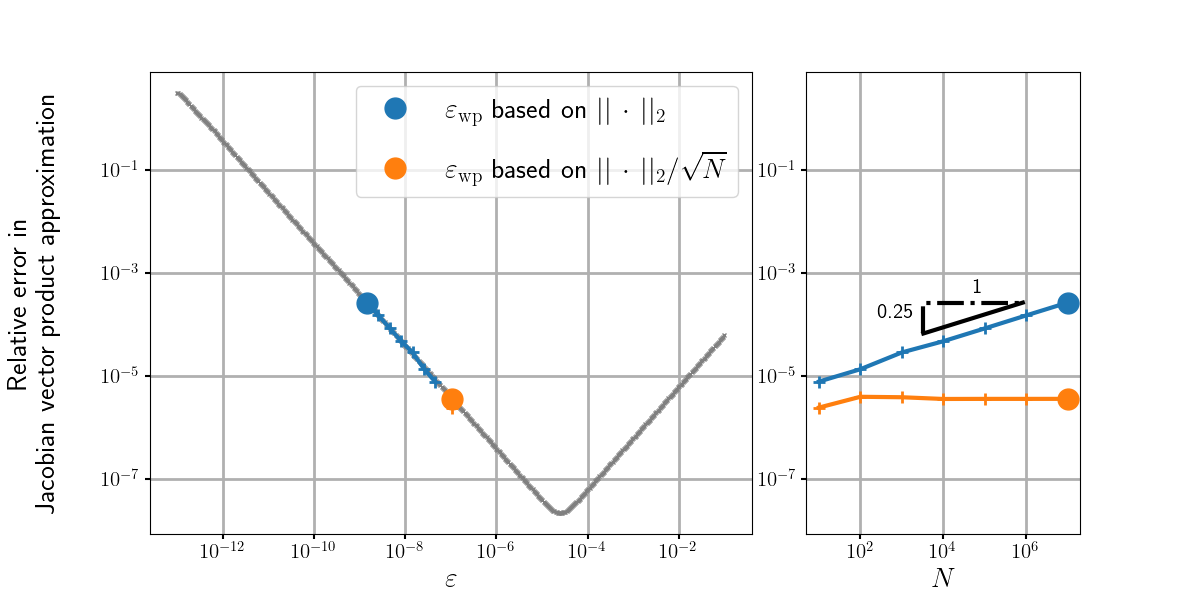
\includegraphics[width=\textwidth]{figures/epsilon_Euler.png}
        \caption{
          Error in the Jacobian matrix vector product approximation as a function on $\varepsilon$ (left) and of the dimension $N$ (right).
          The function is the right-hand side of equation (\ref{eq:ode}) from a Finite Volume method using a centered scheme for the Euler equations over a regular 1D mesh.
          On the left figure, colored cross markers correspond to the values computed on a mesh of $10^1$, $10^2$, ... cells, and circle markers to the last value with $10^7$ cells.
          Grey cross markers on the left figure correspond to a mesh of $10^7$ cells.
        }
        \label{fig:epsilon_euler}
      \end{figure}

      \paragraph{}
      Figure \ref{fig:epsilon_euler} shows the corresponding results.
      As for the previous experiment, $\varepsilon_\textrm{wp}$ depends on the dimension $N$, and then the associated error ends up increasing as $N$ grows.
      Our correction $\varepsilon_{\textrm{wp}, N}$ does not exhibit the same drawback.
      Even if it does not fall at the bottom of the error curve, it at least does not lead to a larger error.

      \paragraph{}
      In this late case, we see that at the beginning the two errors were close.
      In the first one, their starting position were a bit different.
      This is largely due to the randomness of this analysis: the one used to construct the $x$ and $v$ vectors.
      In fact, it would be unwise to draw conclusion from the position of the points in figures \ref{fig:epsilon_burgers} and \ref{fig:epsilon_euler}.
      Changing the choice of vectors, or the function $f$, or even the randomness in the vectors is enough to modify their position.
      For example, we can not conclude anything from the fact that $\varepsilon_\textrm{wp}$ is almost at the bottom of the error curve in figure \ref{fig:epsilon_burgers}.
      It may as well be a bit mort en the side.
      What we can use from this analysis, however, is the tendencies that choices of $\varepsilon$ show.
      The main conclusion is then that with our strategy we removed a dependency of the relative error on the dimension, which makes sense as this dependency is not expected a priori.

      \paragraph{}
      The issue of this analysis is that it relies on extremely simple examples.
      The function $f$ in our actual applications is in fact much more complicated than the two we used here.
      But in order to do this analysis we need to be able to compute the relative error, and this means we need to be able to compute a Jacobian matrix vector product analytically.
      Unfortunately this is not possible for our applications.
      If it was, we would not even need to introduce the approximation (\ref{eq:matrix_free}) and therefore to do this analysis.


  \chapter{Analysis of the Jacobian-Free Newton--Krylov method in CEDRE}
\chaptermark{Analysis of the JFNK method in CEDRE}

\begin{tcolorbox}[title=Résumé du chapitre : Analyse de la méthode JFNK dans CEDRE, colframe=black!50!white]
  \paragraph{}
  Le but de ce chapitre est de vérifier les gains apportés par l'ajout de la méthode JFNK dans le solveur CEDRE.
  Il s'agit de comparer les performances de cette nouvelle méthode avec les méthodes préexistantes en matière de stabilité, robustesse et rapidité.
  Nous adaptons pour cela le point de vue d'un utilisateur, en considérant ce qui l'intéresse lorsqu'il réalise une simulation stationnaire.

  \paragraph{}
  Pour cela, nous comparons tout d'abord la méthode JFNK avec la méthode utilisant explicitement la Jacobienne.
  Cette comparaison se traduit principalement par la comparaison de la convergence des deux méthodes à travers la norme des résidus.
  Ainsi, nous réalisons cette comparaison sur une succession de cas tests, de complexité croissante, sélectionnés car ils représentent différentes facettes du solveur.

  \paragraph{}
  Nous commençons par un calcul purement aérodynamique d'un profil d'aile en deux dimensions dans un écoulement turbulent, qui utilise une modélisation des effets turbulents de la couche limite.
  Puis, nous utilisons le même profil mais cette fois en incidence, avec un maillage bien plus fin qui capture les effets de couche limite turbulente, plutôt que de la modéliser.

  \paragraph{}
  Nous regardons ensuite un cas de rentrée atmosphérique avec une sphère placée dans un écoulement à haute énergie.
  Cela se traduit par un très fort choc, ainsi qu'une zone de déséquilibre thermodynamique où ont lieu d'intenses réactions chimiques.
  Dans un premier temps, nous regardons comme précédemment les deux méthodes pour comparer leur convergence.
  Pour finir, nous utilisons un modèle de fluide récemment ajouté au solveur afin de représenter le déséquilibre thermodynamique.
  Avec les développements réalisés actuellement sur ce nouveau modèle, il n'est pas possible d'utiliser la méthode implicite préexistante, et les utilisateurs sont forcés d'employer des méthodes explicites.
  Nous montrons donc que la méthode JFNK peut elle être utilisée en l'état, sans nécessiter de développements supplémentaires, et permet d'accélérer les calculs ainsi que d'obtenir une meilleure convergence.
\end{tcolorbox}


  \paragraph{}
  In a previous chapter, we identified some methods from the literature that we wanted to use in our solver CEDRE, and some others from CEDRE that we wanted to improve.
  In another chapter, we discussed the practical implementation of said methods in the solver.
  The goal of this chapter is now to test those methods on several applications to comment on the choices we made.
  We need to define test cases that represent well enough target applications so we can comment on the performances of our choices.


  \section{Comparaison entre la matrice jacobienne explicite et la formulation sans matrice}
  \GP{Comparison between full-Jacobian matrix and matrix-free formulations}

    \paragraph{}
    From the previous analysis and implementation, the main addition to the solver is the Jacobian-Free Newton--Krylov method, and in particular the matrix-free approach.
    In this part, the new method that uses the matrix-free approach will be compared with the implicit Euler method as the interest is focused on implicit time integration schemes.
    The traditional method linearises the equation that the implicit Euler method produces, approximates the Jacobian matrix using the Jacobian matrix of the corresponding first-order scheme, and then solves the linear system with the Krylov subspace method GMRES.
    In order to understand the impact of a better Jacobian matrix, the only difference is how the Jacobian matrix is handled.
    The new method will then work in a similar way, except the matrix used in the linear solver is not actually computed, but the matrix-vector products are approximated using equation (\ref{eq:matrix_free}).


    \subsection{Turbulent transonic airfoil}

      \subsubsection{Definition of the test case}

        \paragraph{}
        The first application is a typical aerodynamics test case.
        It is a two-dimensional simulation of the flow around an RAE 2822 wing profile.
        The fluid is standard air assumed to be a perfect gas.
        The Mach number is taken equal to 0.75, the chord is equal to $1\si{\meter}$, the angle of attack is $0\si{\degree}$ and we use the atmospheric conditions at 10km.
        This gives a laminar Reynolds number of \num{6.5e6}.

        \paragraph{}
        This first test case is chosen for multiple reasons.
        Firstly, it is a simple case in the field of computational fluid dynamics.
        It is a standard aerodynamics case, with a small mesh in comparison to many other three-dimensional cases.
        This allows to test our methods inexpensively.
        Secondly, this case belongs to the tutorial suite of our solver.
        It means that it is already well mastered by the team.
        Thirdly, even if it is only a standard aerodynamics case it still has some stiff features, such as turbulence modelling and a shock.
        Finally, it is a standard test case for turbulence modelling validation.
        Therefore there are many references in the literature using this case.

        \paragraph{}
        The mesh used for this simulation is an unstructured hybrid mesh made of triangles and quadrangles.
        Parts of it can be seen in figure \ref{fig:rae_mesh}.
        Cell sizes range from $2.5\si{\meter}$ far from the airfoil and $100\si{\micro\meter}$ at the wall.
        At the wall, there is a C-shaped layer of regular cells.
        This helps better capture boundary layer effects near the profile and the wake.
        Also, under those conditions, a shock is expected to develop on the upper part.
        Special treatment such as refinement was applied to the mesh at the expected shock location.

        \begin{figure}
          \centering
          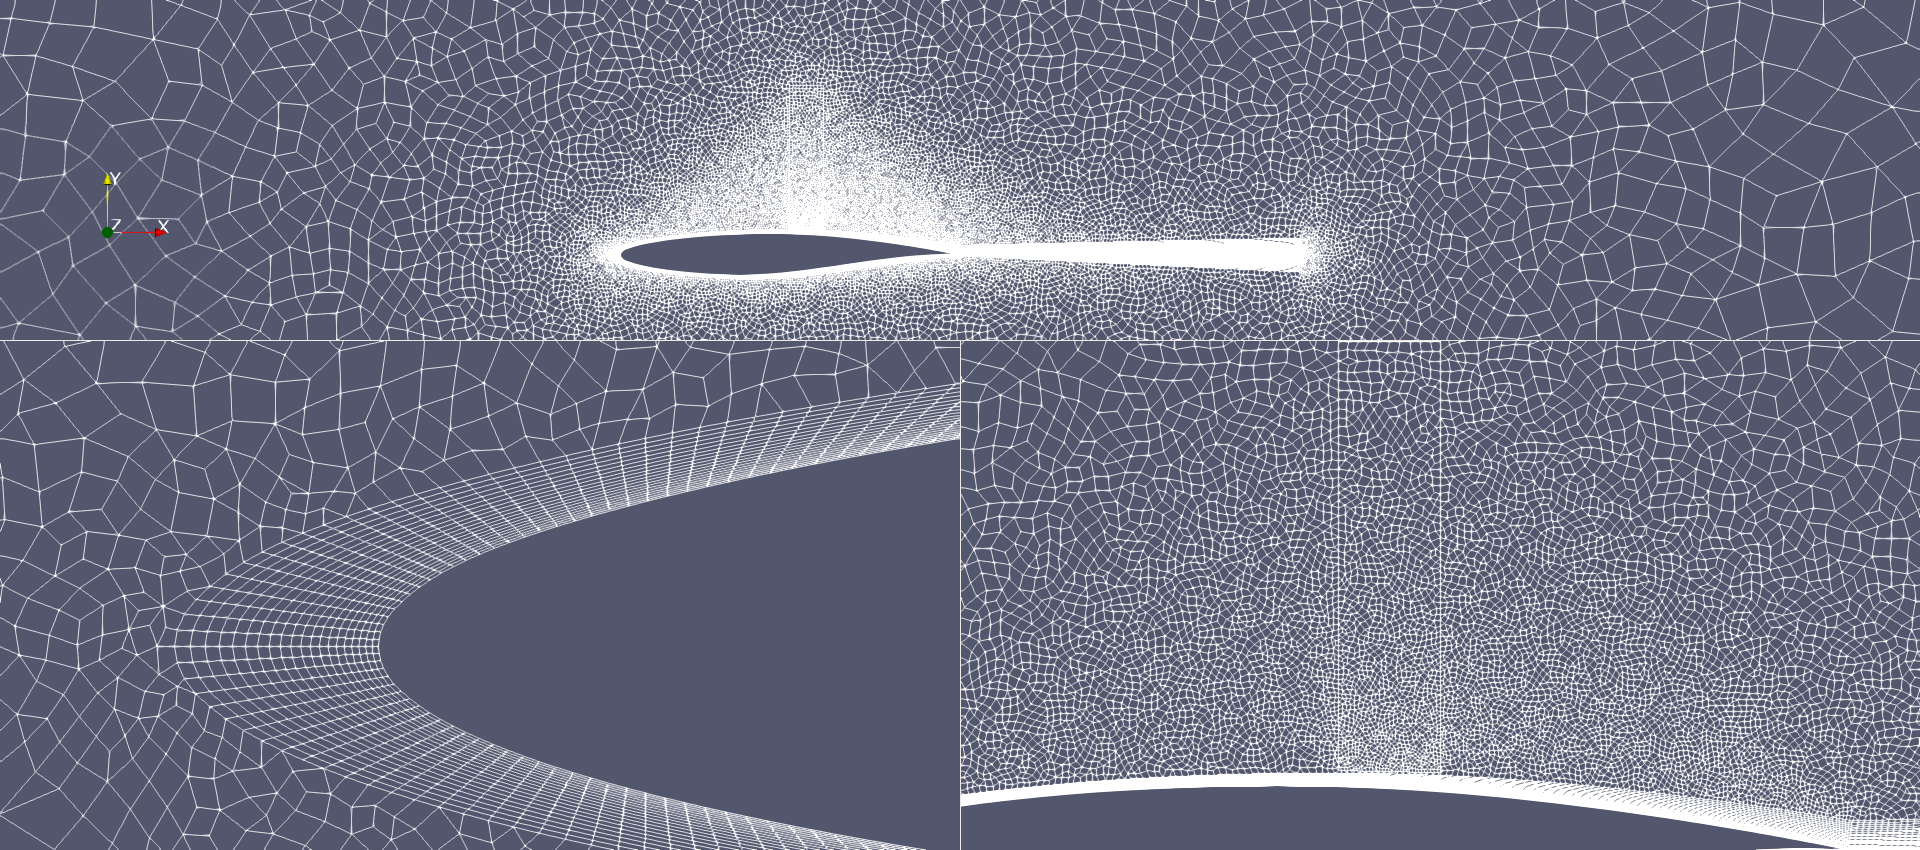
\includegraphics[width=\textwidth]{figures/rae_mesh.png}
          \caption{Mesh for the RAE 2822 test case. Close up on the leading edge and on the expected shock location.}
          \label{fig:rae_mesh}
        \end{figure}

        \paragraph{}
        The model used is the Reynolds Averaged Navier--Stokes equations, or RANS.
        Simply put, every scale of the turbulence is modelled.
        The Spalart--Allmaras turbulence model is chosen to close the RANS equation.
        It is well known for being one of the simplest turbulence models, which is fine to set up a simple first test case.
        Figure \ref{fig:rae_mesh} shows that the mesh near the wall boundary is not particularly fine, and therefore it is not fine enough to compute the boundary layer.
        It is indeed because this computation uses turbulence wall model that replaces the standard no-slip boundary condition by a more complex relation between the variables and their derivatives.
        Physics of the boundary layer is introduced in the model, which limits the stiffness of the system.
        Such models are known to be troublesome with some more complex turbulence models such as the $k-\epsilon$ model but are used with others such as the one we use here.
        Turbulence wall modelling may be nonconventional in aerodynamic simulations but it is a commonly used feature of our solver, so it is interesting to see how our new method behaves on such test cases.
        The spatial discretisation method is a second-order Finite Volume method, using the HLLC Riemann solver and Multislope method \cite{LeTouzeMurroneGuillard2015} with a Van--Leer slope limiter.
        Local time-stepping is used to speed up the convergence.


      \subsubsection{Analysis of the results}

        \paragraph{}
        We are now going to compare the results from the two different simulations.
        It is first worth noting that before trying the JFNK method, the computation needs to start using the traditional method.
        As explained before, the matrix-free approximation is not ideal to handle discontinuities such as shocks, and a shock is indeed present in this computation.
        Only some iterations are needed, just to start the development of the boundary layer and approximately place the shock.
        After that, the computation can be continued, with the traditional method on one side and with the new method on the other.

        \begin{figure}
          \centering
          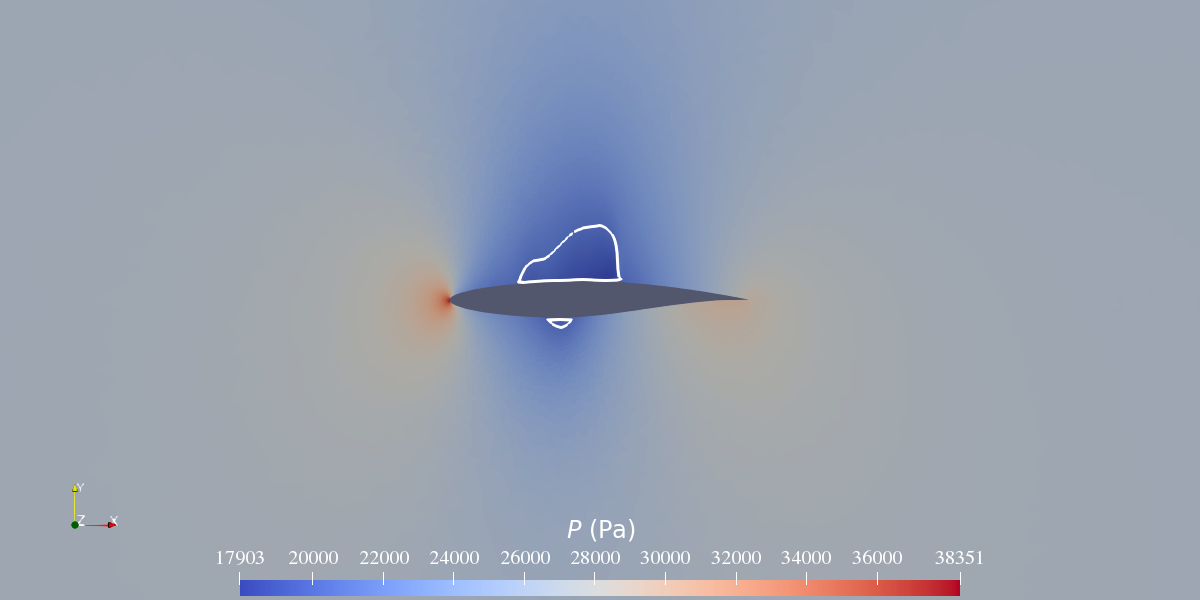
\includegraphics[width=\textwidth]{figures/rae_field.png}
          \caption{Pressure around the RAE 2822 airfoil and sonic $\operatorname{Ma} = 1$ contour.}
          \label{fig:rae_field}
        \end{figure}

        \begin{figure}
          \centering
          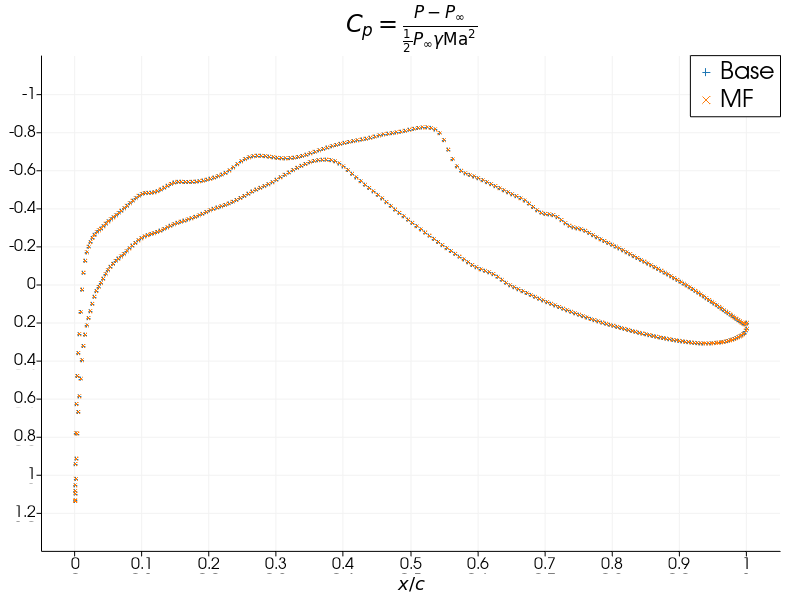
\includegraphics{figures/rae_cp.png}
          \caption{Pressure coefficient around the airfoil for the traditional method (blue) and the JFNK method (orange).}
          \label{fig:rae_cp}
        \end{figure}

        \begin{figure}
          \centering
          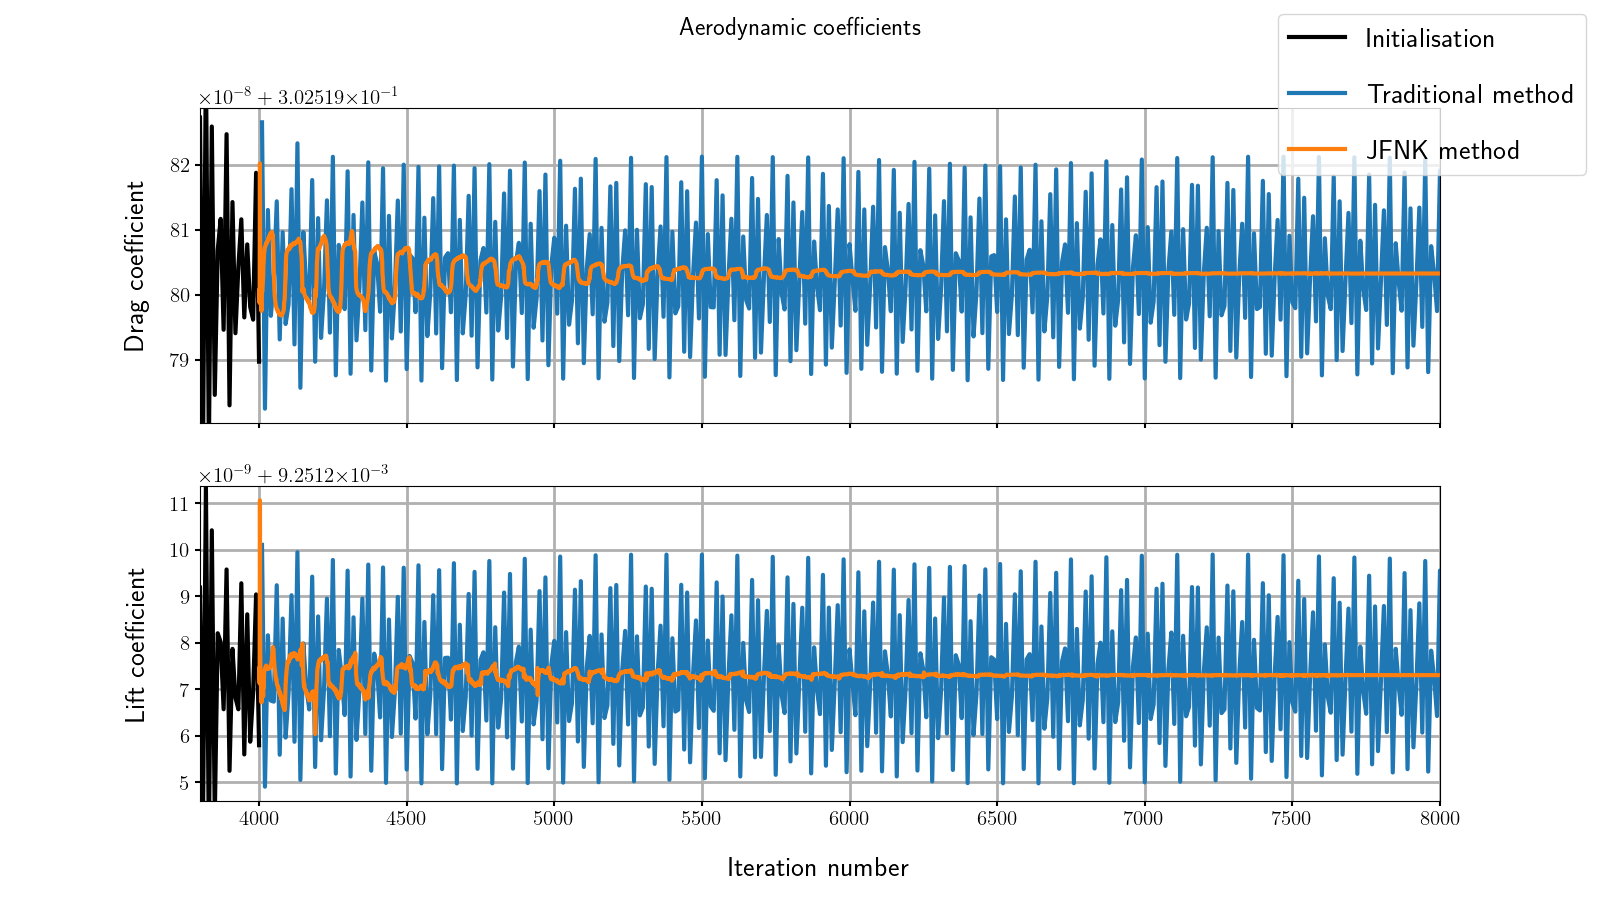
\includegraphics{figures/rae_coefficients.png}
          \caption{Aerodynamic coefficients (lift and drag) for the profile throughout the computation.}
          \label{fig:rae_coefficients}
        \end{figure}

        \paragraph{}
        The global flow is shown in figure \ref{fig:rae_field} through the pressure field near the airfoil.
        The shock is clearly seen on the upper part.
        The two computations give similar results: they are indistinguishable by just looking at the pressure field.
        This is to be expected as the traditional method gives already satisfying results on such applications.
        The pressure coefficient around the airfoil is given in figure \ref{fig:rae_cp}.
        Once again, the two curves are indistinguishable.
        Finally, the aerodynamic coefficients, the drag and lift coefficients, are given throughout the simulation in figure \ref{fig:rae_coefficients}.
        This time, the JFNK method gives an improvement: the coefficients are much more stable, which means the convergence is better.
        The blue curve corresponding to the traditional method struggles to converge and seems to oscillate periodically.
        In comparison, the oscillation of the orange curve is dampened: this corresponds to convergence.
        The scale of the oscillation seen in figure \ref{fig:rae_coefficients} is not significant physically speaking, as it is negligible.
        It shows an issue with the traditional implicit method of the solver CEDRE: it fails to reach proper convergence but it oscillates around the solution.
        The new JFNK method however achieves proper convergence.
        Even if the figure shows an advantage of the new method, the result is almost meaningless as the oscillation of the blue curve is numerically insignificant.
        Looking at other data is necessary to properly conclude on the convergence of the two methods.


        \paragraph{}
        The residual is the best way to measure if a method can help the convergence of the solver.
        To define the residuals, let us use the partial differential equation (\ref{eq:pde}).
        The residual is in fact the value of the function $\operatorname{F}$ from this equation.
        The name is quite adequate: for steady problems, the residual is what is left and still needs to be removed to find a steady solution.
        To decide on the convergence of a steady simulation, this residual norm is measured throughout the computational domain $\mathcal{D}$.
        More precisely, this residual is analysed component by component.
        For example, the residual 1-norm associated with the $i$th component is:
        \begin{equation}
          \norm[1]{\operatorname{F}_i} = \int_\mathcal{D} \left| \operatorname{F}_i \right| \mathrm{d}v
        \end{equation}
        and the $\infty$-norm is:
        \begin{equation}
          \norm[\infty]{\operatorname{F}_i} = \max_\mathcal{D} \left| \operatorname{F}_i \right| .
        \end{equation}
        In this fluid dynamics application, the residual norm is associated with the conservative variables: the density, the momentum components, the energy and the turbulent eddy viscosity $\nu_t$.
        With the Spalart--Allmaras compressible model, the conservative variable in in fact the product of the density and the Spalart--Allmaras variable $\rho \tilde{\nu}$.

        \begin{figure}
          \centering
          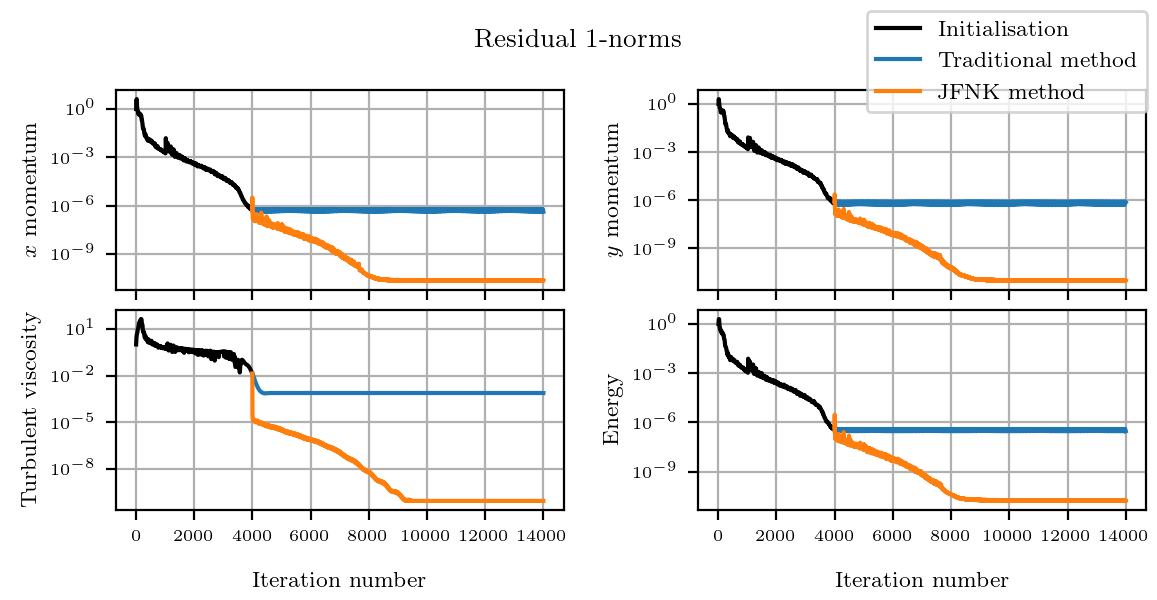
\includegraphics{figures/rae_residuals.png}
          \caption{Residual 1-norms for the two momentum components, energy and turbulent viscosity throughout the computation for the turbulent transonic airfoil case.
          Values are normalised by the initial residual.}
          \label{fig:rae_residuals}
        \end{figure}

        \paragraph{}
        Figure \ref{fig:rae_residuals} shows the residual norms from both computations.
        The gain from using the JFNK method appears clearly.
        The final residual norm is much smaller for each and every conservative component.
        This means that the Jacobian-Free Newton--Krylov method is able to reach a better convergence level than the traditional method.
        In other words, the better Jacobian matrix approximation leads to a better convergence than the older poor approximation.

        \paragraph{}
        In this first test case, we looked at the residual norms as the fields computed by both methods were almost identical.
        Moreover, our method was even able to reach better convergence levels.
        This validates our method on a first simple case, albeit with turbulence modelling and a shock.


    \subsection{Turbulent transonic airfoil with boundary layer resolution}

      \subsubsection{Definition of the test case}

        \paragraph{}
        The previous case uses a mesh that is too coarse to resolve the boundary layer but instead uses a turbulent wall model.
        It is representative of CEDRE applications, but not of actual applications from the aerodynamic community.
        The RAE 2822 airfoil is often used for turbulence model validations, but computations in the field prefer to use a finer mesh to resolve the boundary layer.
        This is what we present next.
        The new mesh, shown in figure \ref{fig:rae_mesh_fine} is clearly different.
        It is a three-dimensional mesh, which is in fact a two-dimensional mesh that was extruded on 6 cells in the $y$ direction.
        Periodicity is set between the two parallel sides of the domain.
        The mesh is made of \num{198144} cells whereas the previous RAE 2822 mesh was only made of \num{36541} cells.
        With these additional cells, this mesh is able to be fine on the wall boundary condition as seen in figure \ref{fig:rae_mesh_fine}.
        This means that the use of the turbulent wall model is no longer necessary, unlike in the previous test case.
        Turbulence closure is still provided by the Spalart--Allmaras one equation turbulence model.
        The scale of the mesh is the same: the chord is still equal to $1\si{\meter}$.

        \begin{figure}
          \centering
          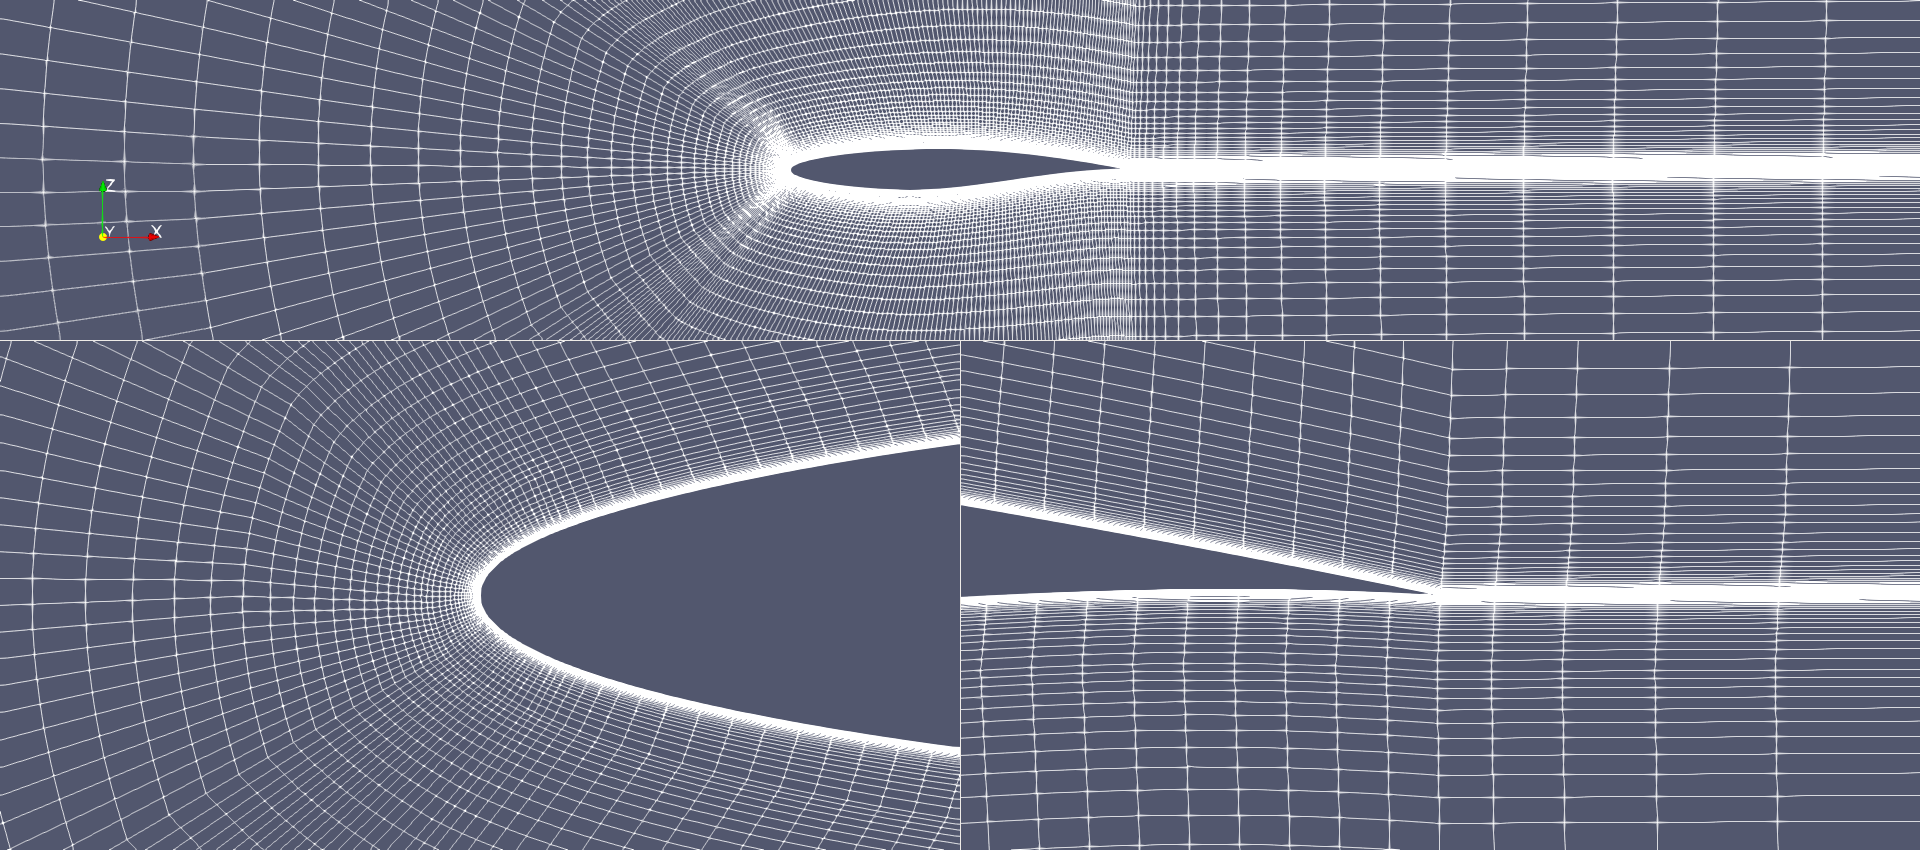
\includegraphics[width=\textwidth]{figures/rae_mesh_fine.png}
          \caption{Finer mesh for the RAE 2822 test case. Close up on the leading and trailing edges.}
          \label{fig:rae_mesh_fine}
        \end{figure}

        \paragraph{}
        The flight conditions are also modified to match some existing experimental conditions: the AGARD-AR-138 experimental database.
        The Mach number is then 0.734 and the angle of attack is $2.54\si{\degree}$, with a Reynolds number of \num{6.5e6}.
        This corresponds to \emph{Case 9} from the experimental conditions.
        The parameters are not exactly the same as they are corrected to account for the effects of the wind tunnel \cite{HellstromDavidsonRizzi1994}.


      \subsubsection{Analysis of the results}

        \paragraph{}
        As before, the computation starts from an initial state constant in the domain.
        Then the computation is continued for a few more iterations with the traditional implicit Euler method.
        This is to reach a state close enough of the steady solution more quickly before analysing the convergence of our methods.
        After that, the computations are restarted, with the traditional method on one side and the matrix-free method on the other.
        The residuals are given in figures \ref{fig:rae_residuals_fine_l1} and \ref{fig:rae_residuals_fine_linf}.
        Overall, it takes much more iterations to decrease residual norms on this test case compared to the previous one.
        It is due to the larger number of cells, and the presence of small flattened cells in the boundary layer.

        \paragraph{}
        Figure \ref{fig:rae_residuals_fine_l1} shows that the reduction in residual 1-norms with the standard method is not satisfying.
        Users usually expect the solver to reduce the order of magnitude of the residuals by 4 or 5, which is more than what our solver does.
        In contrast, the matrix-free method reduces residual norms much more efficiently, and converges to a more precise solution.
        The quality of the solution computed by the matrix-free method is then better.

        \begin{figure}
          \centering
          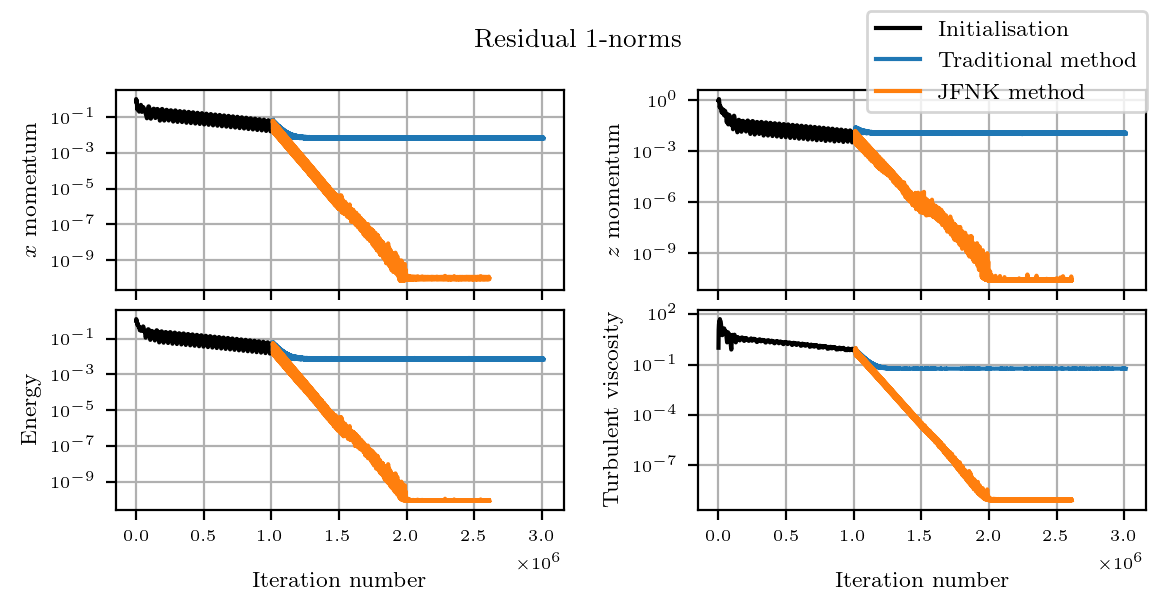
\includegraphics{figures/rae_residuals_fine_l1.png}
          \caption{Residual 1-norms for the horizontal and vertical momentum components, energy and turbulent viscosity throughout the computation for the turbulent transonic airfoil with boundary layer resolution case.
          Values are normalised by the initial residual.}
          \label{fig:rae_residuals_fine_l1}
        \end{figure}

        \paragraph{}
        The $\infty$-norm of the residual is given in figure \ref{fig:rae_residuals_fine_linf} for the same simulations.
        This time, the traditional method is not able at all to reduce residual norms.
        It means there are some cells in the computational domain for which the method is not able to reduce the local residual.
        The JFNK method in orange does not have this issue and converges to a better solution.
        The width of the curve is only due to data noise, as all lines use the same width.

        \begin{figure}
          \centering
          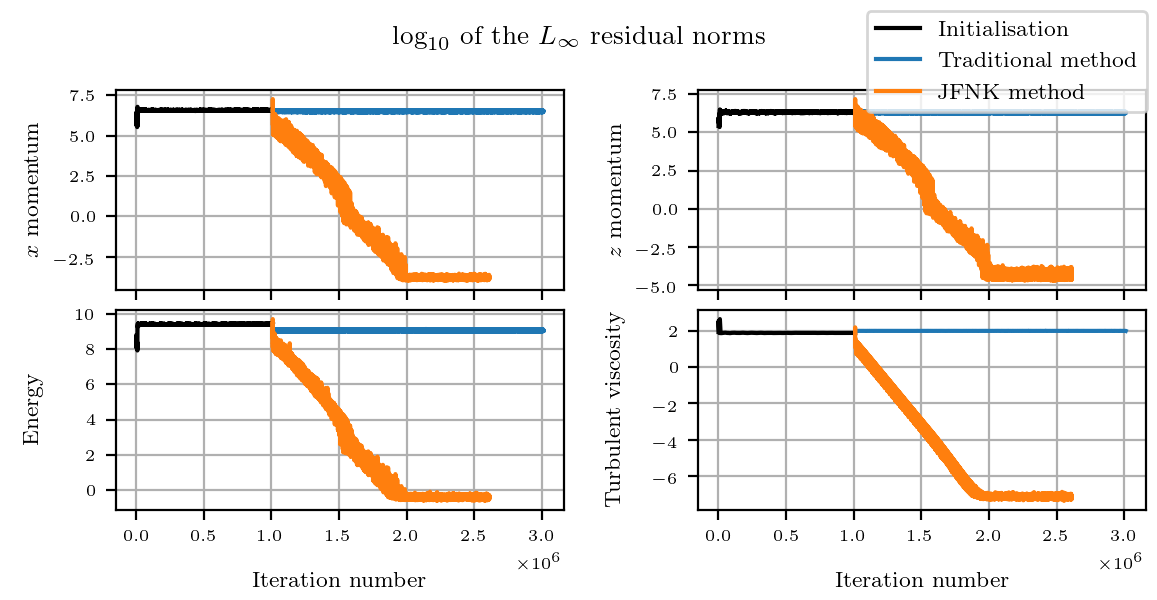
\includegraphics{figures/rae_residuals_fine_linf.png}
          \caption{Residual $\infty$-norms for the horizontal and vertical momentum components, energy and turbulent viscosity throughout the computation for the turbulent transonic airfoil with boundary layer resolution case.
          Values are normalised by the initial residual.}
          \label{fig:rae_residuals_fine_linf}
        \end{figure}

        \paragraph{}
        The value of the turbulent variable $\tilde{\nu}$ in the first cell above the wing profile is provided for both computations in figure \ref{fig:rae_field_fine}.
        The top views show the upper part of the airfoil, and the discontinuity due to the shock is visible, as expected.
        The bottom views show the lower part of the airfoil.
        The views on the right correspond to the JFNK computation, whereas the ones on the left to the computation with the traditional method.
        This traditional method using an approximated Jacobian matrix produces a solution of lower quality, as the pattern is not physical.
        In particular, there are cells for which $\tilde{\nu}$ is null in the computational domain, which should not happen with the standard Spalart--Allmaras model.
        Figure \ref{fig:rae_residuals_fine_linf} shows that the $\infty$-norm of the residual on the conservative variable $\rho \tilde{\nu}$ normalised by the initial residual is near $10^0$, so figure \ref{fig:rae_field_fine} highlights cells for which the residual is higher than $10^{-0.1}$.
        Those cells correspond to the ones for which $\tilde{\nu} = 0$.
        It shows a flaw of the standard time integration method, as it has non-physical features in the solution that prevent the residual convergence.
        In contrast, it shows the quality of the JFNK method on this application.

        \begin{figure}
          \centering
          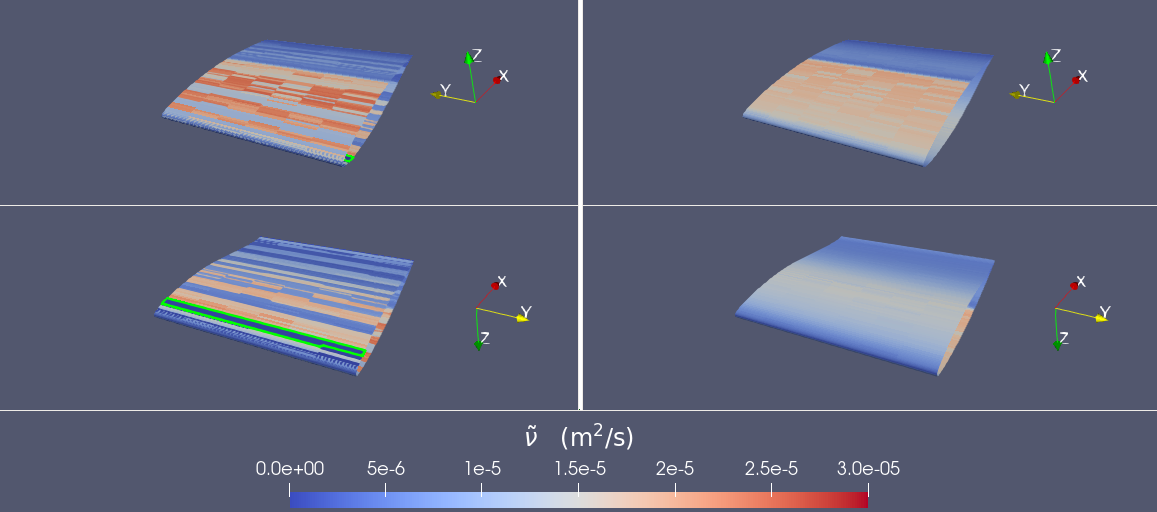
\includegraphics[width=\textwidth]{figures/rae_field_fine.png}
          \caption{
            Spalart--Allmaras variable $\tilde{\nu}$ on the RAE 2822 wing profile for the traditional method (left) and the JFNK method (right).
            The top views show the profile from above, and the bottom views from below.
            The highlighted region in green corresponds to cells where the absolute value of the residual on $\rho \tilde{\nu}$ is higher than $10^{-0.1}$.
          }
          \label{fig:rae_field_fine}
        \end{figure}


    \subsection{Hypersonic reactive sphere}

      \paragraph{}
      The second application we selected to compare the Jacobian-Free Newton--Krylov with the traditional one is the computation of the flow around a hypersonic solid sphere.
      Because of the high energy of the surrounding flow, the air molecules can separate and even form a plasma.
      The hypersonic reactive sphere is a well-known case, for both experimental \cite{Lobb1964} and numerical studies \cite{DobrovGimadievKarpenkoEtAl2022}.
      This is a simple yet representative test case of CEDRE applications.
      It then makes a lot of sense to analyse our new method on it.

      \subsubsection{Definition of the test case}

        \begin{figure}
          \centering
          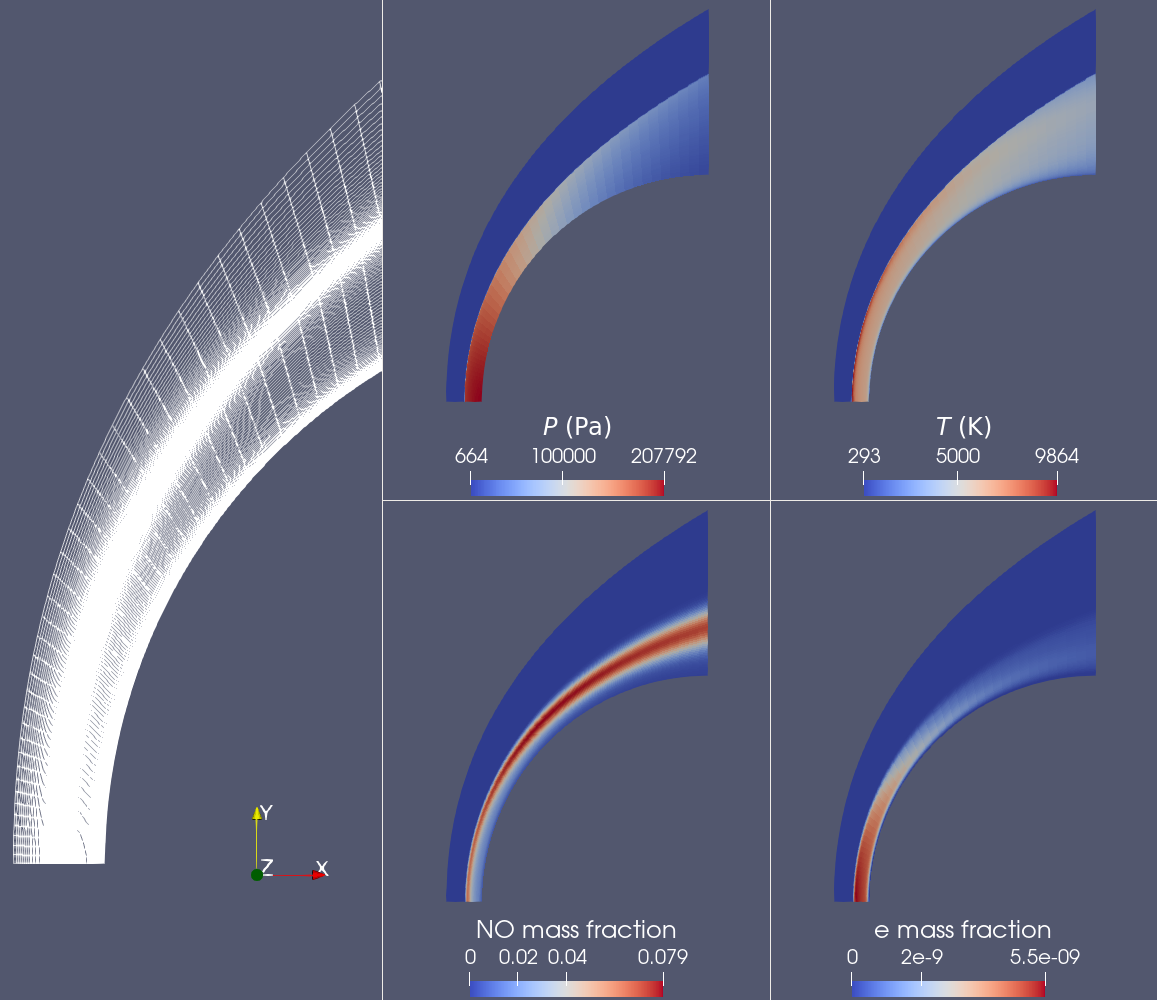
\includegraphics[width=\textwidth]{figures/sphere_fields.png}
          \caption{Mesh along with final pressure, temperature, and \ce{NO} and \ce{e} mass fractions for the hypersonic reactive sphere test case.}
          \label{fig:sphere_fields}
        \end{figure}

        \paragraph{}
        The two-dimensional mesh is shown in figure \ref{fig:sphere_fields}.
        It is a regular mesh made of quadrangles, with refinement in the radial direction at the wall boundary and at the expected shock location.
        The refinement at the wall boundary helps to compute more precisely the physical phenomena that happen at said boundary.
        The refinement at the shock is a requirement of the spatial discretisation methods.
        In order to get a clean and slim shock, the cells near the shock must have a high aspect ratio.
        The mesh takes this into account and is made according to CEDRE best practices.
        This expected shock location is obtained from a previous computation, made with a coarser mesh.
        This mesh is used in a two-dimensional axisymmetric computation to get the flow around a three-dimensional solid sphere.

        \paragraph{}
        The solid sphere is modelled by an isothermal wall boundary condition.
        This is a representative choice as well, as the heat flux going through the wall is one of the main interests of such computation.
        Moreover, as it depends on the derivatives of the flow variables, it is usually harder to get a correct value for the heat transfer.
        A better convergence will lead to better derivatives, which will lead to better physical results for such case users.
        No turbulence model is used, as the flow is mostly laminar.

        \paragraph{}
        The main feature of this test case is that it simulates a hypersonic flow.
        At the left, the input boundary condition feeds air at Mach 15.
        This will induce a strong shock, meaning a strong discontinuity in the flow.
        Is is indeed seen in figure \ref{fig:sphere_fields} on the pressure and temperature.
        As this is a typical application of our solver, it is of importance to us that the new method behaves well with such flow features.
        When going through a strong shock, the temperature of the flow will increase a lot.
        The flow is made of air, or a mixture of 77\% \ce{N_2} and 23\% \ce{O_2}.
        At the high temperature they reach after the shock, the molecules can decompose into \ce{N}, \ce{O}, and \ce{NO}.
        They can even get ionised.
        The choosen model uses 11 possible species: \ce{N_2}, \ce{O_2}, \ce{N}, \ce{O} and \ce{NO}, the corresponding cations \ce{N_2^+}, \ce{O_2^+}, \ce{N^+}, \ce{O^+} and \ce{NO^+} and the electrons \ce{e^-}.

        \begin{figure}
          \centering
          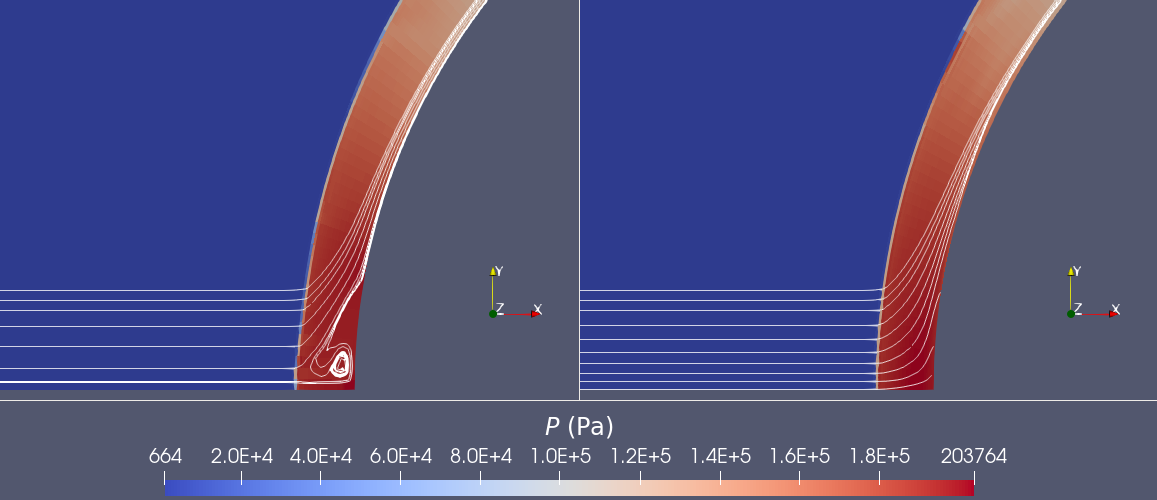
\includegraphics[width=\textwidth]{figures/sphere_carbuncle.png}
          \caption{Streamlines near the stagnation point for two Riemann solvers.}
          \label{fig:sphere_carbuncle}
        \end{figure}

        \paragraph{}
        We argued previously that our solver is quite complex and that it makes it hard to do correct computations for non-experimented users.
        This hypersonic reactive sphere is a perfect example of this statement.
        Even if this case looks simplistic, it should not be taken lightly.
        When using unfit spatial discretisation methods, we ended up with a well-known problem of a such simulation called carbuncle \cite{MacCormack2013}.
        This phenomenon does not come from physics but is solely due to numerical methods.
        It is shown in figure \ref{fig:sphere_carbuncle} from some earlier computations that were using a different mesh.
        Simply put, it creates a recirculation bubble downstream of the shock, near the stagnation point.
        This bubble tends to push the shock farther from the sphere, and modify greatly the heat flux at this location.
        The choice of the Riemann solver ended up being the key element to getting rid of this undesirable effect: there is no recirculation with the AUSM+ scheme.
        There are other pitfalls regarding this test case in CEDRE.
        For example, the user can choose whether to interpolate the mass fraction $y_i$ for the species at the cell interfaces for the MUSCL scheme or the mass concentration $\rho y_i$.
        Choosing the default option leads to nonconverging residuals no matter the time integration method.
        Indeed, this default option is recommended when running simulations with multiple phases, with significant variations in the density.
        Because CEDRE is made to solve a large variety of problems, it has a lot of methods that come with a lot of parameters, so even a simple simulation such as this one requires a lot of knowledge if a good convergence is required.

        \paragraph{}
        This test case is a typical application of CEDRE, as opposed to the previous one which focuses more on the aerodynamic properties.
        Indeed CEDRE does not try to be a pure aerodynamic solver but a multiphysics one, equipped to solve high-energy problems.
        Reentry phenomena are therefore in the scope of our solver.
        Any improvements coming from our method on such applications would benefit a lot of CEDRE users on their applications.


      \subsubsection{Analysis of the results}

        \paragraph{}
        Once again, a first computation is done using the more robust traditional method.
        Indeed, the flow in the first cell against the sphere and the symmetry axis is initialised with a Mach number of 15 going straight into the wall.
        The matrix-free approximation struggles with such stiff initialisations, which is why the computation must start with another method, just until the shock has started to detach from the wall.
        Practically this amount to just a few iterations, compared to the number required to achieve convergence.

        \paragraph{}
        We first look at the different fields from the two computations.
        Once again they are similar and the residual norms are used to compare them, and this shows the simulation accounts for the features of interest.
        In figure \ref{fig:sphere_fields}, we see that the shock is present and that it falls as expected in the refined region.
        We see in the same figure the mass fraction of the various species downstream of the shock, which means the simulation is actively computing the chemical features of the flow, as expected.
        \PS{Comparaison distance corps shock avec \cite{Lobb1964} ?}

        \paragraph{}
        To analyse the result from this case, one might once again look at the residuals.
        The first result correspond to a computaion without reactive model.
        This simplification makes sense as the case to better understand the behaviour of the methods on an easier problem in terms of numerical complexity.
        It also means a different mesh is used, as not accounting for ionisation means the shock location is slightly different, but the two meshes are built the same way.
        The residual 1-norms are shown in figure \ref{fig:sphere_residuals}.
        It shows that the new method gives a better convergence.
        The difference between the traditional method and the new one is that the traditional method uses the Jacobian matrix of the first-order spatial discretisation method, whereas the new one approximates the true Jacobian matrix using the approximation (\ref{eq:matrix_free}).
        This can indeed be verified.
        Because this simulation does not use complex models, the poor approximation used in the traditional model should use the Jacobian matrix of the first-order scheme.
        If the approximation (\ref{eq:matrix_free}) uses the first-order evaluation of $f$, then it should approximate this same Jacobian matrix.
        The evolutions of the residual norms from this method match the ones from the traditional method in figure \ref{fig:sphere_residuals}.
        It first validates the development of the matrix-free approximation, and that the unbridle method should then use the actual second-order Jacobian matrix.
        It also confirms that the traditional method uses the Jacobian matrix of the first-order spatial discretisation method.
        Finally, it validates the choice of $\varepsilon$ and the matrix-free approximation, as it is able to give the same result as when we use the Jacobian matrix.

        \paragraph{}
        With the new method, using the true function $f$ with a second-order lead to much smaller residual norms.
        The only difference between this method and the previously existing one is that the latter uses the Jacobian matrix of the first-order spatial discretisation method, but the JFNK method takes into account the MUSCL reconstruction when using the Jacobian matrix.
        Because it uses a better Jacobian matrix in the linear solve, it gives a better solution to the nonlinear solve, which gives in turn a better time integration.
        It confirms that using a better Jacobian matrix helps the overall convergence when solving steady problems and validates the choice of the Jacobian-Free Newton--Krylov method.

        \begin{figure}
          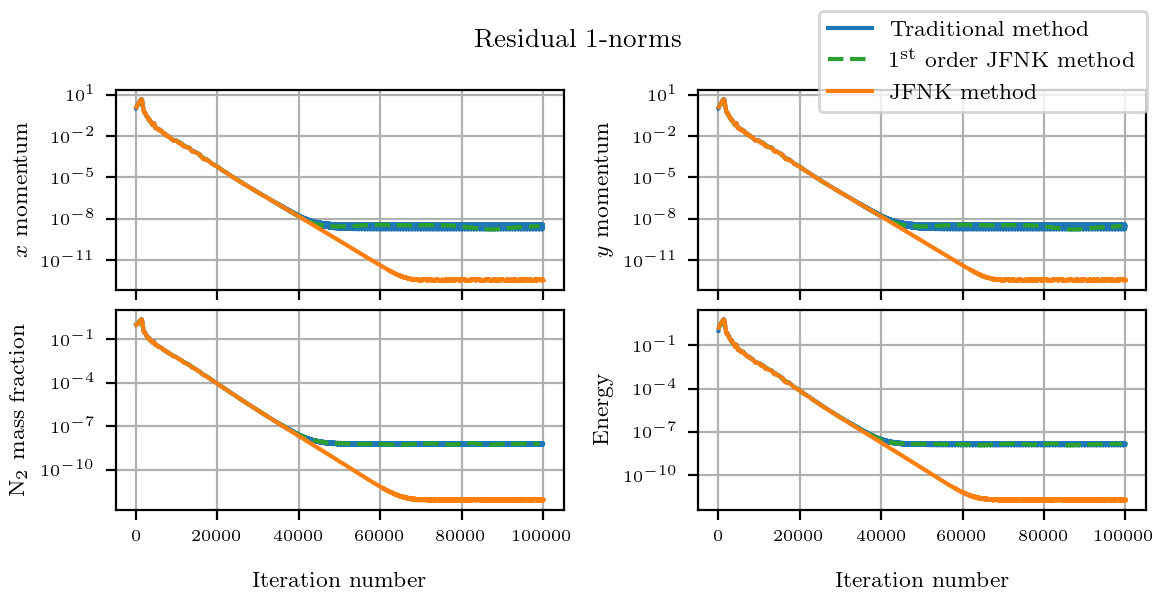
\includegraphics{figures/sphere_residuals.png}
          \caption{Residual 1-norms for the horizontal and vertical momentum components, energy and \ce{N_2} mass throughout the computation for the hypersonic non-reactive sphere case.
          Values are normalised by the initial residual.}
          \label{fig:sphere_residuals}
        \end{figure}

        \paragraph{}
        When adding the reactive model, the conclusion is not in favor of the JFNK method anymore.
        The evolution of the residual norms are shown in figure \ref{fig:sphere_reac_residuals}.
        This time, the JFNK method does not longer find smaller residuals than the traditional method.
        In fact, when comparing figures \ref{fig:sphere_residuals} and \ref{fig:sphere_reac_residuals}, it appears that the traditional method converges better, enough so that it converges better than the JFNK method.
        This appears to happend because the mesh quality is better in this computation, compared to the mesh used without reactive model.
        However, understanding the mesh quality is hard even on this simple test case for the reconstruction methods used in CEDRE.
        This is under current investigation by the responsible team.
        Still, the difference in the convergence of both method is relatively small.
        A possible interpretation of this result is that when the mesh is not ideal for the spatial discretisation methods, using the JFNK method leads to a better convergene as it uses more precise Jacobian matices for the linear system.
        When the mesh quality is better, the JFNK method is slightly less converged.
        Overall, it is still an improvement of the convergence on such test cases.

        \begin{figure}
          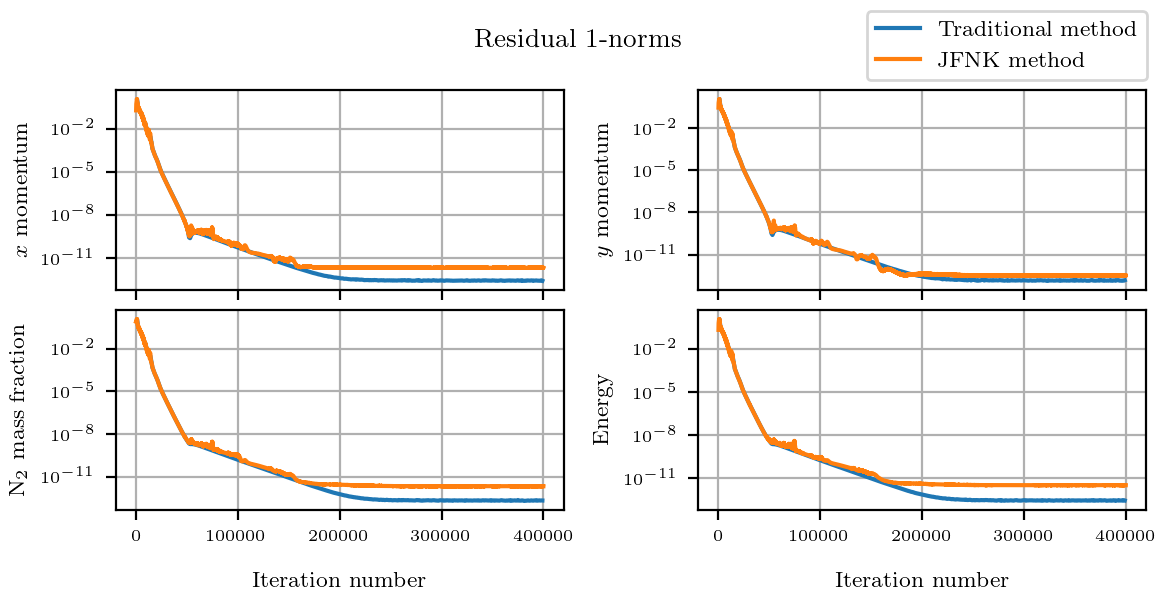
\includegraphics{figures/sphere_reac_residuals.png}
          \caption{Residual 1-norms for the horizontal and vertical momentum components, energy and \ce{N_2} mass throughout the computation for the hypersonic reactive sphere case.
          Values are normalised by the initial residual.}
          \label{fig:sphere_reac_residuals}
        \end{figure}

    \paragraph{}
    In a previous part, we suggested that the poor quality of the Jacobian matrix used in our solver was an obstacle to achieving good convergence.
    We then proposed an improvement: the Jacobian-Free Newton--Krylov method using the matrix-free approximation (\ref{eq:matrix_free}).
    We compared this new method with the traditional one on simple yet representative applications of our solver.
    This comparison showed that indeed, using a better Jacobian matrix leads to a lower residual norm.
    The new method can be useful when looking at quantities that require precise convergence, for instance, the derivatives of the flow variables.
    However, the main drawback of this new method is its computational cost.
    This cost is not inherent to the method but comes from our solver properties as was discussed previously.
    The recommended usage is then to start a computation using the inexpensive traditional method, and then achieve better convergence using the more precise yet more expensive new method.


  \section{Utilisation de la formulation sans matrice sur un nouveau modèle de fluide}

    \paragraph{}
    In the previous section, the new Jacobian-Free Newton--Krylov method was compared to the traditional method that uses the first-order Jacobian matrix.
    This first-order matrix is easily computed for the usual Navier--Stokes equations.
    But as CEDRE is under constant development, new models are added in order to handle more finely various multiphysics phenomena.
    For example, a new model was recently added to better handle multiphasic flows \cite{Cordesse2020}.
    \LM{mais du coup tu ne l'utilises pas du tout ce nouveau modèle dans la suite, non?}
    \PS{Nope c'est juste pour montrer que c'est quelque chose qui se fait, et donc que le Matrix free peut intéresser d'autres personnes.}
    Adding a new model amount to writing the function $\operatorname{F}$ from equation (\ref{eq:pde}), or equivalently $\operatorname{G}$ from equation (\ref{eq:ode}).
    Usually, the development of this function is straightforward as it is given explicitly from the equations.
    However, the development of the Jacobian matrix is much more difficult.
    This is why the new models can not compute Jacobian matrices, and therefore can not use implicit methods.
    \LM{Je dirais plutôt qu'on ne se précipite pas sur l'effort d'évaluation du jacobien, pas qu'on ne peut pas l'évaluer, non?}
    \PS{Concretement, on ne peux pas évaluer la jacobienne de MF5 et MTE, donc les deux ?}
    The Jacobian-Free Newton--Krylov method is then a nice way to use implicit methods as it does not require the Jacobian matrix.
    Because the matrix-free approximation is written in a generic fashion, it can be used on any fluid model.
    In the following, we will use the JFNK method on a new fluid model that does not have an available Jacobian matrix and therefore can not use traditional implicit methods.


    \subsection{Multi-TEmperature model}

      \paragraph{}
      The new model we will use is called the \emph{Multi-TEmperature model}, or MTE.
      Its difference from the traditional Navier--Stokes model is that it allows for a thermodynamic non-equilibrium of some flow components.
      A particle has multiple degrees of freedom: translation, rotation and vibration.
      In more traditional models, it is assumed that all modes are at equilibrium, and they are grouped in what we call energy.
      One can define a time constant for each energy mode that corresponds to the number of collisions that are required to get to the equilibrium.
      A few collisions are required for translation modes, and about ten for rotation modes.
      This gives a small time constant of order $10^{-9} \si{\second}$.
      For vibration modes, however, up to \num{20000} collisions are required.
      The corresponding time constant is significantly larger, and there may be regions where there can be a disequilibrium between vibrational energy on one side and translation and rotation energy on the other.
      The energy of such components can no longer be described with a single temperature.
      As electrons are much lighter, they move more than the other heavier flow components.
      Their transitional energy and the transitional energy of other components can not be described with the same temperature.
      With the new Multi-TEmperature model, the flow components may be divided into three classes:
      \begin{itemize}
        \item the ones that always are at the equilibrium
        \item the ones that may be at vibrational disequilibrium
        \item the electrons that are handled separately from the other heavy component.
      \end{itemize}

      \paragraph{}
      To account for the disequilibrium, the Navier--Stokes equations (\ref{eq:ns}) are modified into the following:
      \begin{equation}
        \left\{\begin{alignedat}{5}
          &\partial_t\left(  \rho_s  \right) &&+ \nabla\cdot\left(  \rho_s \vec{u}  \right) &&=
            \nabla\cdot\bigl( \rho D_s \nabla y_s\bigr) + \dot \omega_s \\[10pt]
          %
          &\partial_t\left(  \rho \vec{u}  \right) &&+ \nabla\cdot\left(  \rho \vec{u} \otimes \vec{u}  +  \left(p + p_e\right) \mat{\operatorname{Id}}  \right) &&=
            \nabla\cdot\biggl(
              \mu \left(\nabla \vec{u} + \nabla \vec{u}^T\right)
              - \frac{2}{3} \mu \left(\nabla \cdot \vec{u} \right) \mat{\operatorname{Id}}
            \biggr) \\[10pt]
          %
          &\partial_t\left(  \rho_m e_{v,m}  \right) &&+ \nabla\cdot\left(  \rho_m e_{v,m} \vec{u}  \right) &&=
            \nabla\cdot\bigl(
              \lambda_{v,m} \nabla T_{v,m}
              + \rho e_{v,m} D_m \nabla y_m
            \bigr) \\
            &&&&& \phantom{= {}} + S^{v-t}_m + S^{v-v}_m + S^{v-e}_m + \dot \omega_m e_{v,m} \\[10pt]
          %
          &\partial_t\left(  \rho_e e_e  \right) &&+ \nabla\cdot\left(  \left(\rho_e e_e + p_e\right) \vec{u}  \right) &&=
            \nabla\cdot\bigl(
              \lambda_e \nabla T_e
              + \rho h_e D_e \nabla y_e
            \bigr)
            + \vec{u} \cdot \nabla p_e \\
            &&&&& \phantom{= {}} + S^{e-t} + S^{e-r} + S^{e-v} + \dot \omega_e e_e \\[10pt]
          %
          &\partial_t\left(  \rho E  \right) &&+ \nabla\cdot\left(  \left(\rho E + p + p_e\right) \vec{u}  \right) &&=
            \nabla\cdot\Biggl(
              \lambda_{eq} \nabla T
              + \sum_m \lambda_m \nabla T_m
              + \lambda_e \nabla T_e \\
              &&&&& \phantom{=\nabla\cdot\Biggl(} + \mu \left(\nabla \vec{u} + \nabla \vec{u}^T\right) \vec{u} - \frac{2}{3} \mu \left(\nabla \cdot \vec{u}\right) \vec{u} \\
              &&&&& \phantom{=\nabla\cdot\Biggl(} + \rho \sum_s h_s D_s \nabla y_s
            \Biggr)
        \end{alignedat}\right.
      \end{equation}
      The first noticeable feature is that the equations of this physical model are more complex compared to the standard Navier--Stokes equations.
      Futrthermore, there are multiple energies corresponding to the multiple temperatures: $e_e$ the energy of the electronic gas, $e_{v, m}$ the vibrational energy for each flow component that may be at disequilibrium, and $E$ the total energy.
      It increases the number of conservative variables.
      The variables $y$ correspond to the mass fraction of the different flow components.
      The source terms $\omega$ correspond to chemical production or decay.
      The source terms $S$ correspond to the energy transfers between the different energy modes.
      The details of those terms can be complex and are not discussed here as it is not the subject of this thesis, but can be found in \cite{Soubrie2006}.
      A noticeable feature of this model is the presence of a nonconservative term in the conservation equation of the electrons' energy: $\vec{u} \cdot \nabla p_e$.
      This term is due to the effect of the electric field.
      This is a known issue of this model, as the Finite Volume method handles better conservative terms.
      Some work tried to transform this equation into a conservative one by using the electronic entropy instead of energy but by neglecting dissipation terms concerning the electrons \cite{CoquelMarmignon1995}.
      \LM{Je ne comprends pas la phrase..}
      \PS{Des travaux ont tenté de la rendre conservative en utilisant l'entropie des electrons comme variable conservative au lieu de leur énergie. A reformuler avec toi}
      However, this simplification can lead to inaccuracy in the physical result, and it appears that using the nonconservative formulation is necessary to get physically accurate results \cite{Soubrie2006, KimGuelhanBoyd2012}.
      Not to go into too much detail, such models that account for thermodynamic disequilibrium are still under discussion as of today \cite{BlancoJosyula2020}.

      \paragraph{}
      The Multi-TEmperature model allows for non-equilibrium between the vibrational mode of the flow components, the electronic energy and the total energy.
      Taking this non-equilibrium into account helps to compute more precisely physical quantities such as the electronic density, which can be useful for magnetohydrodynamics applications for example.
      It gives a better prediction of shock layer radiation with a better representation of the population of energy states which helps the simulation of radiation cooling or the computation of wall heat fluxes.
      This model is most interesting on reentry problems, as there is indeed some non-equilibrium downstream of the strong shocks that appear on such problems.
      Taking the non-equilibrium into account can change the flow downstream of the shock and on the solid wall, and give more precise temperatures and chemical compositions.
      Generally speaking, the Multi-TEmperature model gives more precise results than the standard Navier--Stokes model on fast flow with low relative density where there may be some thermodynamic non-equilibrium, such as reentry problems or problems with the strong expansion of a plume.


    \subsection{Hypersonic reactive sphere}

      \paragraph{}
      The hypersonic sphere test case is a perfect fit for the Multi-TEmperature model.
      There is some thermodynamic non-equilibrium in the region downstream of the shock, because of its intensity.
      Unfortunately, the Jacobian matrix for the new MTE model is not currently available.
      This limits the MTE model users to explicit time integration methods, and therefore small time steps for stability reasons.
      As they deemed explicit time integration too slow, they wanted to use the newly implemented Jacobian-Free Newton--Krylov method for their simulations.
      We will show in the following another interest of the matrix-free approximation: it allows for implicit time integration methods despite having no Jacobian matrix.
      The goal here is to be able to get a steady solution to the problem as fast as possible for the user.
      Initially, the MTE model users were using a second-order Runge--Kutta method: the Midpoint method.
      We will compare the JFNK method to this reference method, and we will look in particular at how much time is required from the user to get to a physically satisfying result.


      \subsubsection{Full reactive model}

        \paragraph{}
        For the first step of our analysis, we will use the most complete physical model.
        We use the same 11 flow components as before: \ce{N_2}, \ce{O_2}, \ce{N}, \ce{O} and \ce{NO}, the corresponding cations \ce{N_2^+}, \ce{O_2^+}, \ce{N^+}, \ce{O^+} and \ce{NO^+} and the electrons \ce{e^-}.
        We of course use the Multi-TEmperature model, and we consider that \ce{N_2} and \ce{O_2} may be at vibrational disequilibrium.
        Other components may in fact also be at disequilibrium and we could take them into account but the computational cost increase is not worth it.
        As they are less present, and they quickly get to the equilibrium relatively to \ce{N_2} and \ce{O_2}, accounting for their disequilibrium would not be significant in the results \cite{Park2006}.
        This amount to having four temperatures to describe the flow: $T_e$ for the electrons, $T_{v, \ce{N_2}}$ and $T_{v, \ce{O_2}}$ for the vibration modes of \ce{N_2} and \ce{O_2}, and $T$ for the total energy.

        \paragraph{}
        As before, the Jacobian-Free Newton--Krylov method needs some help at the beginning.
        This is why the computation starts with some iterations of the Midpoint method and uses the first-order Finite Volume method.
        Then, it continues with the JFNK method, still using the first-order Finite Volume method, to quickly get a good enough approximation of the expected solution.
        \LM{Pour les premières itérations avec la "midpoint method", on est à l'ordre 1 en espace ou pas?}
        \PS{Oui, c'est précisé}
        \LM{Et pour le passage au JFNK, l'ordre 1 c'est pour tout le schéma spatial, ou juste pour l'approximation de l'action de la matrice?}
        \PS{Tout, je dis qu'on utilise la méthode FV d'ordre 1, ça m'a pas l'air ambigu, je dois mieux préciser ?}
        Finally, to get a finer result, the simulation uses the second-order spatial discretisation method.
        Local time-stepping based on the CFL number is used.
        \LM{je ne sais plus si c'est possible, mais il y a-t-il du pas de temps local pour les simulations "explicites"}
        \PS{Non, pourquoi ?}
        The GMRES method can not use preconditioners that require the matrix, so the only one available is the diagonal preconditioner based on the cell volumes.
        It is not ideal as it is extremely simple, and some physics-based preconditioner would be preferable \cite{KnollKeyes2004} but none were available to us at the time.
        The spatial discretisation method used is the Multislope method, as it appears more robust than the $k$-exact method with the Multi-TEmperature model.

        \paragraph{}
        The goal of this thesis is not the physical analysis of this test case so it will be left out, but according to the MTE model users, the results are in agreement with the literature.
        We show in figure \PS{TODO} the various temperatures along the symmetry axis.
        This justifies the use of the Multi-Temperature model: the region downstream of the shock is indeed in a thermodynamic non-equilibrium state.
        \PS{Hypothétique : Comparaison AET MTE}

        \paragraph{}
        We will also look at the residuals for this analysis.
        But this time, we will not be using the number of iterations as the $x$-axis as it will be unfair to the explicit method.
        Indeed the cost of one iteration is a lot smaller for the explicit method than for the implicit JFNK one.
        What matters to us and a typical user is not the number of iterations but the time spent waiting for the result.
        It is called the elapsed real time or wall-clock time.
        As we will run our computations each time in the same parallel environment, with a fixed number of CPU cores, the elapsed time is proportional to the CPU time.
        The $x$-axis will then be the CPU time: the actual time it took to get to the current residual.

        \begin{figure}
          \centering
          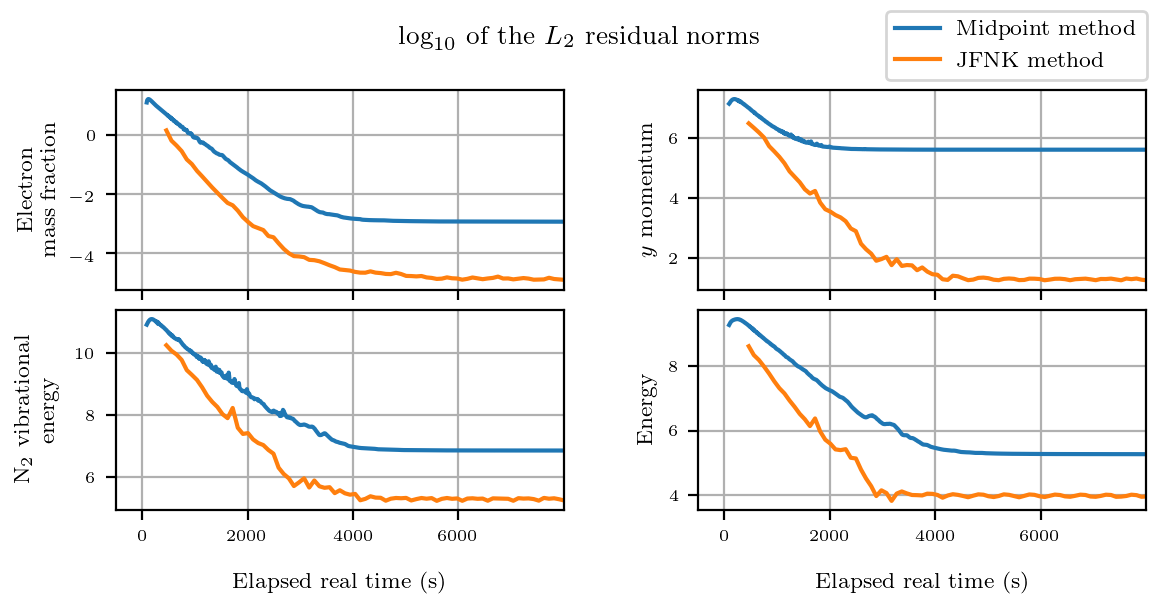
\includegraphics{figures/sphere_mte_residuals.png}
          \caption{Residual 1-norms for the electron mass fraction, vertical momentum, \ce{N_2} vibrational energy and total energy for the Multi-TEmperature model computation throughout the computation.
          Values are normalised by the initial residual.}
          \label{fig:sphere_mte_residuals}
        \end{figure}

        \paragraph{}
        Figure \ref{fig:sphere_mte_residuals} shows the residual norms for the two computations.
        The leftmost black curve corresponds to the initialisation: a few iterations of the explicit time integration method.
        From then we can continue the computation with the Midpoint method on one side and the Jacobian-Free Newton--Krylov method on the other.
        We see that the residual norm obtained with the JFNK method is lower than its explicit counterpart.
        Indeed, the explicit method is limited to small time steps because of the shock and the stiff reactive model.
        \PS{C'est sûr ça ? Parce que l'explicite n'a même pas l'air de bouger ...}
        The implicit method however is not.
        The fact that the implicit method can use larger time steps is not new, but with this specific model, it was not possible to use implicit methods until we added the matrix-free approximation.
        The JFNK method even ends up being cheaper in terms of CPU time.
        This means that for a user, it is faster to use the newly implemented Jacobian-Free Newton--Krylov method than to use explicit methods.
        Our method gives a better alternative to users working on problems with the Multi-TEmperature model.


      \subsubsection{Simplified reactive model}

        \paragraph{}
        The equations concerning electrons in the Multi-TEmperature model bring a lot of issues.
        It is because the quantity of free electrons is usually relatively small when compared to other flow components.
        It can lead to numerical instabilities or cause other problems.
        As the equations hold everywhere in the numerical domain, they hold in particular in areas without free electrons, upstream of the shock in our hypersonic sphere for example.
        The question one must ask is then how to compute quantities such as the electronic temperature $T_e$ where there are no free electrons.
        We will not go into such implementation details as it goes beyond the scope of this work, but the point is that having electrons is quite troublesome for numerical methods.
        According to users that work on such reentry applications, it is not always useful to compute fluid ionisation.
        We explained why it might be crucial for some simulations, but when we do not look at the electrons, their effect on other quantities is almost negligible.
        Those users said that \PS{"ça craint de dire "il a dit que" ?"} \LM{Ben, si tu peux juste dire que l'on peut parfois se satisfaire des degrés de liberté d'energie de vibration en occultant ceux des électrons et que ça donne déjà des infos intéressantes en allégeant et simplifiant drastiquement le numérique, c'est déjà un peu plus vendeur, non?}it is acceptable, meaningful and still useful to do the same simulation but ignoring electrons.
        It is done by considering only the chemical components \ce{N_2}, \ce{O_2}, \ce{N}, \ce{O} and \ce{NO}.

        \paragraph{}
        We decided to do the same comparison as before but this time with the simplified reactive model.
        We once again start the computation with a few iterations of the Midpoint method and use that as a common initialisation.
        Then, we compare the explicit method with the Jacobian-Free Newton--Krylov method.
        We show the corresponding residual norms in figure \PS{TODO}, while still using the CPU time as the $x$-axis.
        The result is similar to the previous one, except it is even more in favour of the JFNK method.
        The implicit method reaches much lower residual norms than the explicit one.
        With the full reactive model, the limiting factor for the implicit method came from the stiffness due to the electrons.\LM{On est sûr que c'est la raideur, ou c'est le fait que l'on patche, lorsqu'il n'y a plus d'électrons, par un raccord non C1?}
        Without them, the convergence is significantly faster.
        The time step for the explicit method however is under the same limitations with both reactive models.
        The gain in CPU time is then huge, in favour of the JFNK method.


\part{Intégration temporelle à grand pas de temps}

    \chapter{Introduction to exponential integration methods}

\begin{tcolorbox}[title=Résumé du chapitre : Introduction aux méthodes d'intégration exponentielles, colframe=black!50!white]
  \paragraph{}
  Le but de ce chapitre est de d'introduire un nouveau type de méthodes d'intégration temporelle.

  \paragraph{}
  Les méthodes classiquement utilisées dans la résolution des problèmes stationnaires sont souvent réutilisées après être adaptées dans la résolution de problèmes instationnaires intégrés avec de grands pas de temps pour s'affranchir des critères de stabilité de l'intégration explicite.
  Nous présentons dans ce chapitre le principe des méthodes d'intégration exponentielles, qui sortent de la dichotomie explicite/implicite.
  Nous décrivons ensuite plus en détail la famille des méthodes Rosenbrock exponentielles, qui seront utilisées par la suite.
  Nous réalisons également une brève analyse théorique de ces méthodes.

  \paragraph{}
  Comme leur nom l'indique, ces méthodes reposent sur l'exponentielle.
  Leur difficulté vient du fait qu'elles nécessitent de calculer des exponentielles de matrices, de très grande taille dans nos applications.
  Nous détaillons donc comment ce calcul est réalisé en utilisant des sous-espaces de Krylov.

  \paragraph{}
  Finalement, nous essayons une méthode exponentielle développée dans CEDRE sur un cas analytique simple.
  Nous montrons alors la pertinence de cette nouvelle méthode au vu de ses performances sur ce cas.
\end{tcolorbox}


  \vspace{1cm}
  \paragraph{}
  In this thesis, we were interested in finding solutions to steady problems.
  As we explained in the previous part, we use implicit time integration methods to efficiently get solutions to such problems.
  This is a pretty standard choice: most computational fluid dynamics solvers use implicit time integration methods to solve steady problems.
  The reason is that they can use larger time steps than their explicit counterparts.
  Because of this advantage, they are also often used when solving unsteady problems but with large time steps.
  Indeed, solving an unsteady problem with large time steps is similar to solving a steady problem.
  Most of what is done towards the steady problem solve can therefore be reused for unsteady problem with large time steps.

  \paragraph{}
  Even if implicit time integration methods are quite standard when solving problems with large time steps, there are other less conventional methods we could choose from.
  We could step out from the explicit implicit dichotomy, and decide to use IMplicit-EXplicit, or IMEX, methods.
  They split the function from the ordinary differential equation (\ref{eq:ode}) into two parts: the stiff part that is integrated by an implicit method, because of its stiffness, and the other part that can just be integrated with an explicit method.
  The Additive Semi-Implicit Runge--Kutta methods, or ASIRK methods, are such methods \cite{Zhong1996}.
  They are already in use in computational fluid dynamics problems, such as fluid-structure interaction problems \cite{HuangPerssonZahr2019}.
  Previous work already implemented ASIRK methods in our solver CEDRE for specific multiphysics applications.
  Some methods are even less common and correspond to a total paradigm shift: the parallel time integration methods \cite{Nievergelt1964, LionsMadayTurinici2001}.
  Just as we classically split the computational domain over processes and compute the spatial discretisation method in parallel, parallel time integration methods decompose the time integration interval into subintervals.
  They then solve the ordinary differential equation on each interval concurrently then ensure the continuity between the subintervals.
  They then iterate with Newton's method to find the solution over the whole time integration interval.
  As a result, they can approximate accurately the solution at a later time without knowing accurately the solution at a previous time.
  Despite being nontraditional, they were successfully used to solve fluid-structure interaction problems or Navier--Stokes problems \cite{GanderVandewalle2007}.
  They were even more recently used to solve simple turbulent flow problems \cite{Lunet2018}.
  They can even be used in a more convoluted way, with for instance exponential methods \cite{GanderGuettel2013}.
  Just as parallel time integration is inspired by parallel spatial discretisation, some other time integration methods are inspired by spectral discretisation methods.
  Time spectral methods, that were originally used for fluid dynamic time-periodic problems \cite{GopinathJameson2005, GopinathJameson2006}, are now used on non-periodic problems \cite{EkiciDjeddiLiEtAl2020}.
  \PS{GP, pourquoi pas ça :
  But as both time parallel integration methods and time spectral methods are considered modern methods and highly unconventional, they do not seem appropriate for an industrial solver such as ours.
  }
  In this part, however, we prefer to focus on another class of time integration methods.


  \section{Exponential integration methods}

    \paragraph{}
    We focus on methods known as exponential methods.
    Despite being known for a long time \cite{Pope1963}, they were not widely used in computational fluid dynamics, because of some difficulties that we will explain later, but still interested some scientists \cite{EdwardsTuckermanFriesnerEtAl1994}.
    They started to come back in the literature \cite{HochbruckOstermann2005, HochbruckOstermann2010} and are now being used on applications similar to ours \cite{NieZhangZhao2006, BhattKhaliqWade2018}.

    \paragraph{}
    We start with an ordinary differential equation
    \begin{equation}\label{eq:ode_2}
      \frac{\mathrm{d} y}{\mathrm{d} t} = f\left(y\right) .
    \end{equation}
    This is the same as the ordinary differential equation (\ref{eq:ode}) from the previous part but with different notations.
    The main idea of exponential integration methods is to start from the ordinary differential equation (\ref{eq:ode_2}) and split the function $f$ into a linear part and a nonlinear part:
    \begin{equation}\label{eq:ode_split}
      \frac{\mathrm{d} y}{\mathrm{d} t} = Ly + N\left(y\right) .
    \end{equation}
    This decomposition is sometimes natural for some particular equations, but in the more general case it is always possible: it consists in choosing a linear part $L$ and then setting the nonlinear part $N\left(y\right) = f(y) - Ly$.
    There are then an infinite number of decompositions, but we will see later that some are more interesting.

    \paragraph{}
    To define the time integration step, we start from the current estimate of the solution $y_n$ that we assume to be exact: $y_n = y\left(t_n\right)$.
    We note $\Delta t = t_{n+1} - t_n$ as we work here with a fixed $n$.
    We can integrate equation (\ref{eq:ode_2}) using the variation of constants formula to get:
    \begin{equation}\label{eq:ode_int}
      y\left(t_{n+1}\right) = e^{\Delta t L} y_n + \int_{t_n}^{t_{n+1}} e^{\left(t_{n+1} - t\right) L} N\left(y\left(t\right)\right) \mathrm{d}t .
    \end{equation}
    The exponential integration methods then approximate the integral to compute the next value $y_{n+1}$.
    What defines the method is how it approximates this integral.
    As we can see in equation (\ref{eq:ode_int}), the linear part is treated exactly and the nonlinear one is approximated.
    If there is no nonlinear part, with $N = 0$, then the solution $y_{n+1}$ is exact.
    If there is no linear part, with $L = 0$, then equation (\ref{eq:ode_int}) transforms into
    \begin{equation}\label{eq:ode_int_classic}
      y\left(t_{n+1}\right) = y_n + \int_{t_n}^{t_{n+1}} N\left(y\left(t\right)\right) \mathrm{d}t
    \end{equation}
    and the exponential integration method behaves like a standard time integration method.
    This is the advantage of exponential integration methods: at best they are exact methods, and at worst, they are equivalent to traditional methods.

    \paragraph{}
    Similarly to classic methods, there are explicit \cite{BhattKhaliqWade2018} and implicit \cite{NieZhangZhao2006} exponential integration methods.
    It depends on whether it uses $y_{n+1}$ or not to compute the integral from equation (\ref{eq:ode_int}).

    \paragraph{}
    Before continuing, we need to define some functions that are going to be convenient later on.
    We consider the functions $\varphi_k$, defined by:
    \begin{equation}
      \left\{\begin{aligned}
        \varphi_0 &: z \mapsto e^z \\
        \forall k \in \mathbb{N}^*, \varphi_{k} &: z \mapsto \int_0^1 e^{\left(1 - \theta\right)z} \frac{\theta^{k-1}}{\left(k-1\right)!} \mathrm{d}\theta .
      \end{aligned}\right.
    \end{equation}
    We could also define them using the recurrence relation:
    \begin{equation}
      \left\{\begin{aligned}
        \varphi_0 &: z \mapsto e^z \\
        \forall k \in \mathbb{N}, \varphi_{k+1} &: z \mapsto \frac{\varphi_k\left(z\right) - \varphi_k\left(0\right)}{z} .
      \end{aligned}\right.
    \end{equation}
    Finally, we can also use their analytic formula:
    \begin{equation}
      \forall k \in \mathbb{N}, \varphi_{k} : z \mapsto \sum_{i = 0}^{+\infty} \frac{z^i}{\left(i + k\right)!} .
    \end{equation}
    This analytic formula ensures it is well-defined for squared matrices.


  \pagebreak
  \section{Exponential Rosenbrock--Euler method}

    \subsection{Definition of the exponential Rosenbrock--Euler method}

      \paragraph{}
      To better understand exponential integration methods, we take the most basic one: the exponential Euler method.
      Just as the Euler method assumes that $N\left(y\right)$ is constant and equal to $N\left(y_n\right)$ in equation (\ref{eq:ode_int_classic}), its exponential counterpart makes the same assumption but in equation (\ref{eq:ode_int}).
      It then gives:
      \begin{equation}
        y_{n+1} = e^{\Delta t L} y_n + \Delta t \varphi_1\left(\Delta t L\right) N\left(y_n\right)
      \end{equation}
      using the $\varphi_1$ function defined above, and finally:
      \begin{equation}\label{eq:expeuler}
        y_{n+1} = y_n + \Delta t \varphi_1\left(\Delta t L\right) f\left(y_n\right) .
      \end{equation}
      We note the difference with the corresponding standard Euler method, for which the $\varphi_1$ function is replaced with the identity function.
      If there is no linear part in the decomposition, with $L = 0$, then nothing is treated differently by the exponential method, and we recover the standard explicit Euler method.

      \paragraph{}
      In this method, we take the linearisation $L = f'\left(y_n\right)$.
      Because of this choice, the method is called the exponential Rosenbrock--Euler method.
      We will discuss the nomenclature below.
      This choice feels natural and minimises the error of the method as is shown in the following.
      This choice is frequent among exponential integration methods, despite some methods using a fixed linearisation $L = f'\left(y_0\right)$.
      The difference is that a new Jacobian matrix is required at each iteration of the time integration method, but it is something we are used to with our traditional implicit methods.
      It is worth noting that we might want to try the implicit equivalent of this method by taking $N\left(y\right) = N\left(y_{n+1}\right)$ in equation (\ref{eq:ode_int}).
      However, because we took $L = f'\left(y_n\right)$, $N'\left(y\right) = 0$ and after a linearisation the two variants are equivalent.


    \subsection{Analysis of the exponential Rosenbrock--Euler method}

      \paragraph{}
      From the definition of the method and equation (\ref{eq:ode_int}), we have that the error made after one step is:
      \begin{equation}
        \begin{aligned}
          y\left(t_{n+1}\right) - y_{n+1} &= \int_{t_n}^{t_{n+1}} e^{\left(t_{n+1} - t\right) L} N\left(y\left(t\right)\right) \mathrm{d}t  - \Delta t \varphi_1\left(\Delta t L\right) N\left(y_n\right) \\
          &= \int_{t_n}^{t_{n+1}} e^{\left(t_{n+1} - t\right) L} \left( N\left(y\left(t\right)\right) - N\left(y_n\right) \right)
        \end{aligned}
      \end{equation}
      We take the Taylor series of the nonlinearity:
      \begin{equation}
        N\left(y\right) = \sum_{i = 0}^{+\infty} \frac{N^{\left(i\right)}\left(y_n\right)}{i!}\left(y - y_n\right)^i
      \end{equation}
      and in particular, using the fact that
      \begin{equation}
        \begin{aligned}
          y\left(t\right) &= y_n + y'\left(t_n\right)\left(t - t_n\right) + O\left(\left(t - t_n\right)^2\right) \\
          & = y_n + f\left(y_n\right)\left(t - t_n\right) + O\left(\left(t - t_n\right)^2\right)
        \end{aligned}
      \end{equation}
      the partial series of order 2 is:
      \begin{equation}
        N\left(y\left(t\right)\right) = N\left(y_n\right) + N'\left(y_n\right)f\left(y_n\right)\left(t - t_n\right) + O\left(\left(t - t_n\right)^2\right) .
      \end{equation}
      The error of the method is then:
      \begin{equation}
        \begin{aligned}
          y\left(t_{n+1}\right) - y_{n+1} &= \int_{t_n}^{t_{n+1}} e^{\left(t_{n+1} - t\right) L} \left( N'\left(y_n\right)f\left(y_n\right)\left(t - t_n\right) + O\left(\left(t - t_n\right)^2\right) \right) \mathrm{d}t \\
          &= \Delta t^2\varphi_2\left(\Delta t L\right) N'\left(y_n\right)f\left(y_n\right) + O\left(\Delta t^3\right) .
        \end{aligned}
      \end{equation}
      We now understand the decomposition chosen earlier: if $L = f'\left(y_n\right)$ and therefore $N'\left(y_n\right) = 0$ then $y\left(t_{n+1}\right) - y_{n+1} = O\left(\Delta t^3\right)$ and the method is of order 2.
      This is a noticeable property of this method: despite being a single-step method it has a second-order of accuracy.
      A more rigorous analysis can be found in \cite{HochbruckOstermannSchweitzer2009}.

      \paragraph{}
      It is much harder to analyse the stability of this method, and more generally of exponential methods.
      Indeed, the stability analysis is done on the Dahlquist test equation (\ref{eq:dahlquist}).
      But as this equation is linear, exponential methods can solve them exactly no matter the time step size.
      We can still write the single step equation (\ref{eq:single_step}) $y_{n+1} = g\left(\Delta tJ\right)y_n$ with $g\left(z\right) = e^z$, and get the corresponding stability region which is the left half complex plane.
      We could then conclude that the method is A-stable.
      The issue with exponential methods is that the standard stability analysis is no longer pertinent.
      We tried to do a better stability analysis for simple exponential methods such as the exponential Rosenbrock--Euler method, but we did not succeed.
      Some work in the literature does define some stability notions for exponential methods \cite{DuZhu2004}, but usually takes a linear $N$.
      It goes against the idea that all the linear part of $f$ is in $L$ and $N$ is purely nonlinear.
      We did not find a stability analysis that was satisfying to us.


  \section{Exponential Runge--Kutta and Rosenbrock methods}

    \paragraph{}
    When we introduced explicit methods, we used more convoluted approximations than the explicit Euler methods for the integral in equation (\ref{eq:ode_int_classic}).
    This gave the Runge--Kutta methods.
    We can do the same for the integral in equation (\ref{eq:ode_int}) to get exponential Runge--Kutta methods.
    The difference with a standard Runge--Kutta method is that the quadrature coefficients are now functions of the matrix $L$:
    \begin{equation}
      \left\{\begin{aligned}
        y_{n+1} &= e^{\Delta t L} y_n + \Delta t \sum_{i = 1}^k b_i\left(\Delta t L\right) N\left(y_{n,i}\right) \\
        \textrm{with}\quad y_{n,i} &= e^{c_i \Delta t L} y_n + \Delta t \sum_{j = 1}^{i-1} a_{ij}\left(\Delta t L\right) N\left(y_{n,j}\right) .
      \end{aligned}\right.
    \end{equation}
    The Butcher tableau that we used to represent the Runge--Kutta methods is also used to represent the exponential Runge--Kutta methods.
    For instance, the Butcher tableau of the exponential Rosenbrock--Euler method, which is a special simple case of exponential Runge--Kutta methods, is shown in table \ref{tab:exprb_butcher}.

    \paragraph{}
    Until now, we have not been exact when naming the methods we constructed here.
    From the literature, exponential Runge--Kutta methods are defined just as we did above, except they use a fixed linearisation: $L = f'\left(y_0\right)$ \cite{HochbruckOstermann2005}.
    It is because they were developed for semilinear parabolic problems:
    \begin{equation}
      \frac{\mathrm{d} y}{\mathrm{d} t} + Ay = g\left(y\right) .
    \end{equation}
    They are used when the remainder $g$ is small or at least bounded in terms of $A$.
    This is not the case in our applications, and in many others so that is why another type of exponential method was introduced: exponential Rosenbrock methods \cite{HochbruckOstermannSchweitzer2006}.
    They can be seen as a variation of the exponential Runge--Kutta methods where the linearisation is done at each time step.
    The issue is that a new Jacobian matrix is needed at each iteration, but once again we are used to this with implicit methods.

    \paragraph{}
    The nomenclature is a bit blurry to us, as the distinction between exponential Runge--Kutta and exponential Rosenbrock methods is not the same as the one between Runge--Kutta methods and Rosenbrock methods.
    First of all, the exponential Rosenbrock method is not implicit contrary to its standard counterpart.
    Furthermore, it would make sense to us to name an exponential integration method base on the underlying method used to approximate the integral from equation (\ref{eq:ode_int}), and exponential Rosenbrock methods do not use Rosenbrock methods to do it.
    The only parallel we found was that the Rosenbrock methods do a linearisation at each inner stage, and the exponential Rosenbrock methods do a linearisation at each step of the time integration.
    It just seems that in the literature, the term \emph{Rosenbrock} indicates that the linearisation is computed at each step instead of once at the beginning, with no apparent link with Rosenbrock methods.

    \paragraph{}
    Just as the Runge--Kutta method has order conditions for its quadrature coefficients, the exponential Rosenbrock method quadrature functions must follow some rules to ensure the expected order.
    To be consistent, it must have:
    \begin{equation}
      \sum_{i = 1}^k b_i = \varphi_1
    \end{equation}
    and it must also have
    \begin{equation}
       \sum_{j = 1}^{i-1} a_{ij} = z \mapsto c_i \varphi_1\left(c_i z\right), \quad 1 \leq i \leq k
    \end{equation}
    to achieve a second order.
    As we want to use methods with multiple stages, it is reasonable to want them to have a higher order than the single-stage exponential Euler method.
    Using these two conditions, exponential Rosenbrock methods can be written in the form:
    \begin{equation}\label{eq:exprb_defect}
      \left\{\begin{aligned}
        y_{n+1} &= y_n  + \Delta t \varphi_1\left(\Delta t L\right) f\left(y_n\right) + \Delta t \sum_{i = 1}^k b_i\left(\Delta t L\right) D_{n,i} \\
        \textrm{with}\quad y_{n,i} &= y_n  + c_i \Delta t \varphi_1\left(c_i \Delta t L\right) f\left(y_n\right) + \Delta t \sum_{j = 1}^{i-1} a_{ij}\left(\Delta t L\right) D_{n,j}
      \end{aligned}\right.
    \end{equation}
    using $D_{n,i} = N\left(y_{n,i}\right) - N\left(y_n\right)$.
    This form shows that exponential Rosenbrock methods are variations of the exponential Euler method.
    The defects $D_{n, i}$ are small in size, so less computational effort can be spent when computing their contribution.

    \paragraph{}
    Among exponential Rosenbrock methods, we looked at the ExpRB32 method from \cite{HochbruckOstermannSchweitzer2009} and ExpRB42 methods from \cite{Luan2017}.
    They were developed as adaptive methods, but we will use them without the error estimate as standard methods.
    They are both 2-stage exponential Rosenbrock methods and achieve respectively a third and fourth order of accuracy.
    This shows the quality of exponential Rosenbrock methods.
    Their Butcher tableaux are in table \ref{tab:exprb_butcher}.
    We decided to work with those two methods, along with the Rosenbrock--Euler method, as they are simple among exponential methods and are supposedly well suited for our problems.
    They give us methods with orders of accuracy from 2 to 4.
    But what is interesting to us is that on linear problems those methods are exact, or with an infinite order of accuracy.
    As our problems are not purely linear, it means that the linear part will be solved exactly while the nonlinear part will be solved with a still good order of accuracy.

    \begin{table}
      \center
      \begin{tabular}{M{.25\textwidth}M{.3\textwidth}M{.3\textwidth}c}
        \begin{tabular}{c|c}
          \multicolumn{1}{c}{} \\ 0 \RKBar $\varphi_1$
        \end{tabular} &
        \begin{tabular}{c|cc}
          0 \\ 1 & $\varphi_1$ \RKBar $\varphi_1 - 2 \varphi_3$ & $2\varphi_3$
        \end{tabular} &
        \begin{tabular}{c|cccc}
          0 \\ $\frac{3}{4}$ & $\frac{3}{4}\varphi_1\left(\frac{3}{4} \cdot\right)$ \RKBar $\varphi_1 - \frac{32}{9} \varphi_3$ & $\frac{32}{9}\varphi_3$
        \end{tabular} & \\[20pt]
        Exponential Rosenbrock--Euler & ExpRB32 & ExpRB42 \\
      \end{tabular}
      \caption{Butcher tableau for some exponential Rosenbrock integration methods}\label{tab:exprb_butcher}
    \end{table}


  \section{Evaluating matrix functions}

    \paragraph{}
    At first glance, exponential methods may seem too good to be true.
    Indeed, they give explicit methods with few stages but high order of accuracy, and they have the formidable quality that they solve exactly the linear part of the ordinary differential equation.
    In other words, the exponential Euler method should be able to get the solution of Poisson's equation after any time with a single step.
    Indeed, Poisson's equation gives often a linear ordinary differential equation after the spatial discretisation, with the Finite Volume method on a regular mesh for example.
    The exponential Rosenbrock--Euler method can solve this linear differential equation exactly, for any time step, as large as it may be.

    \paragraph{}
    The reason why exponential methods are not that good is the reason why they were not used for a long time after being introduced.
    It is because evaluating matrix exponential, or more generally evaluating the $\varphi$-functions on matrices, is not trivial.
    Indeed, the power series definition of the matrix exponential is not well suited for numerical evaluations.
    In particular, in our context, computing the powers of the matrix is completely out of the question.
    The dimension of our matrices can get large, and the powers of the matrices would lose the sparsity.
    In fact, any approximation working directly with the matrix would not be satisfying.

    \paragraph{}
    The other issue with exponential methods is the question of the Jacobian matrix.
    Exponential Runge--Kutta reuse the same matrix throughout the computation but it is not a good idea in our applications since the nonlinear part can change.
    Exponential Rosenbrock methods were introduced for this reason but they require the computation of a new Jacobian matrix at each iteration.


    \subsection{Evaluating matrix functions with Krylov subspace methods}

      \paragraph{}
      The solution for both issues is the same: Krylov subspace methods.
      The Cayley--Hamilton theorem ensure that the exponential of a matrix is a polynomial of degree less or equal to $N$ where $N$ is the dimension of the matrix.
      Instead of looking for the matrix exponential as an infinite series, we can look for an $N$-order polynomial.
      Moreover, exponential methods do not need to evaluate the exponential or the $\varphi$-functions of the matrix, but their effect when applied to a vector.
      For instance, the exponential Rosenbrock--Euler method from equation (\ref{eq:expeuler}) does not need to compute $\varphi_1\left(\Delta t L\right)$ but $\varphi_1\left(\Delta t L\right)f\left(y_n\right)$.
      It means we do not need to evaluate the function $g$ on the matrix $A$, but to compute the effect of $g\left(A\right)$ on the vector $b$.
      The idea, originally developed to approximate eigenvalues of a large sparse matrix, is to use a Krylov subspace method to approximate $g\left(A\right)b$ \cite{Saad1992, Sidje1998}.
      In fact, it is similar to using a Krylov subspace method to solve the linear system $Ax = b$: it means taking $g = z \mapsto z^{-1}$.
      The Krylov subspace method produces with the Arnoldi iteration the relation, at the $m$-th iteration:
      \begin{equation}\label{eq:arnoldi}
        AV_m = V_{m+1} \tilde{H}_m = V_m H_m + h_{m+1, m} v_{m+1} e_m^T .
      \end{equation}
      The columns of $V_m$, $v_1, \dots, v_m$, form an orthonormal basis of the Krylov subspace:
      \begin{equation}
        \krylov[A, b]{m} = \operatorname{Vect}\left( b, Ab, \dots, A^{m-1}b \right)
      \end{equation}
      with $v_1 = b / \norm[2]{b}$.
      The matrix $\tilde{H}_m$ is a Hessenberg matrix and $H_m$ is the square matrix equal to $\tilde{H}_m$ without its last line:
      \begin{equation}
        \tilde{H}_m = \begin{pmatrix}
          h_{1,1} & h_{1,2} & \cdots    & h_{1,m} \\
          h_{2,1} & h_{2,2} & \cdots    & h_{2,m} \\
          \vdots  & \ddots  & \ddots    & \vdots  \\
          0       & \cdots  & h_{m,m-1} & h_{m,m} \\
          0       & \cdots  & 0         & h_{m+1,m}
        \end{pmatrix} , \quad H_m = \begin{pmatrix}
          h_{1,1} & h_{1,2} & \cdots    & h_{1,m} \\
          h_{2,1} & h_{2,2} & \cdots    & h_{2,m} \\
          \vdots  & \ddots  & \ddots    & \vdots  \\
          0       & \cdots  & h_{m,m-1} & h_{m,m}
        \end{pmatrix}
      \end{equation}
      The vector $v_{m+1}$ is the last column vector of $V_{m+1}$, added to the column vectors of $V_m$ to get an orthonormal basis of $\krylov[A, b]{m+1}$, and $e_m$ is the $m$-th canonical vector $\left(0, \dots, 0, 1\right)^T$.
      Since $H_m$ represent the compression of $A$ on $\krylov[A, b]{m}$ with respect to basis $V_m$ and $b = \norm[2]{b} V_m e_1$ with $e_1 = \left(1, 0, \dots, 0\right)$, we make the approximation \cite{EiermannErnst2006}:
      \begin{equation}
        g\left(A\right)b \approx \norm[2]{b} V_m g\left(H_m\right) e_1 .
      \end{equation}

      \paragraph{}
      With this approximation, we can evaluate the function $g$ by applying it to a smaller matrix.
      We reduced the original function evaluation to the much smaller Krylov subspace.
      Since the method does not need to know the matrix but only to be able to apply it as a linear operator, we can use the matrix-free approximation (\ref{eq:matrix_free}) to approximate the Jacobian matrix $L = f'\left(y_n\right)$.
      This way, having to compute a new Jacobian matrix at each iteration of the exponential Rosenbrock method is not an issue.
      Just as Krylov subspace methods for solving linear problems, this method can be restarted to limit the size of the Krylov subspace and therefore control the memory consumption of the algorithm.
      It is even possible to define an error estimate in our approximation to dynamically control the number of iterations needed to reach a given tolerance, albeit it is more convoluted than the residual used for solving linear systems with Krylov subspace methods \cite{EiermannErnst2006}.

      \paragraph{Note:}
      Since the matrix used to evaluate the quadrature functions of the exponential Rosenbrock methods is always the same, $L$, only one Arnoldi iteration is required for one step of the method.
      This could lead to a great cost reduction, however, we did not try it in our developments.
      Indeed, our work on exponential integration methods was more to demonstrate their feasibility in our applications, but it would be interesting to use this idea for future performance enhancements.


    \subsection{Evaluating matrix exponentials}

      \paragraph{}
      With the Krylov subspace method we just described, we now need to compute the exponential of the smaller Hessenberg matrix $H_m$.
      We now look at how to compute the exponential of relatively small dense matrices.
      Many methods use special properties of the matrices but our matrices do not share the same properties.
      Instead of using a truncated Taylor series, using the Padé approximant seems to be the best option \cite{HighamAlMohy2010}.
      The exponential function is approximated by the $\left[k/m\right]$ Padé approximant:
      \begin{equation}
        e^z \approx r_{k,m}\left(z\right) = \frac{p_{k,m}\left(z\right)}{q_{k,m}\left(z\right)} \quad\textrm{with} \left\{\begin{aligned}
          \quad p_{k,m} &= \sum_{i = 0}^k \frac{\left(k + m - i\right)! k!}{\left(k + m\right)! \left(k - i\right)!} \frac{z^i}{i!} \\
          \quad q_{k,m} &= \sum_{i = 0}^m \frac{\left(k + m - i\right)! m!}{\left(k + m\right)! \left(m - i\right)!} \frac{\left(-z\right)^i}{i!} .
        \end{aligned}\right.
      \end{equation}
      It is best to use diagonal approximants, with $k = m$, as they are more accurate \cite{HighamAlMohy2010}.

      \paragraph{}
      The final method used to compute the exponential of a dense matrix is the Scaling and Squaring method \cite{Higham2009}.
      It computes an optimal parameter $s$ and takes:
      \begin{equation}
        e^z \approx r_{m,m}\left(z/2^s\right)^{2^s} .
      \end{equation}
      The goal is to choose $s$ such as the error on the computation of the exponential is bounded, with minimal cost.
      It then decides on an optimal order $m$ for the Padé approximant.
      The matrix is scaled by $2^s$, the Padé approximant is used to compute the exponential, and the result is then squared back to the original scale.
      It is what gives its name to the method.


    \subsection{Evaluating the \texorpdfstring{$\varphi$}{phi}-functions}

      \paragraph{}
      The exponential time integration methods we introduced do not only use matrix exponential, the $\varphi_0$ function, but may use any $\varphi_k$ function.
      There is a nice relation that helps compute those functions.
      We first define the \emph{augmented} squared Hessenberg matrix:
      \begin{equation}
        \bar{H}_{m + p} = \begin{pmatrix}
          H_m & c & 0 & \cdots & 0      \\
              & 0 & 1 & \ddots & \vdots \\
              &   & 0 & \ddots & 0      \\
              &   &   & \ddots & 1      \\
          0   &   &   &        & 0
        \end{pmatrix}
      \end{equation}
      with a vector $c$ of dimension $m$.
      Then, the following relation holds \cite{Sidje1998}:
      \begingroup
      \renewcommand*{\arraystretch}{1.5}
      \begin{equation}
        \exp\left(\tau \bar{H}_{m + p}\right) = \begin{pmatrix}
          \exp\left(\tau H_m\right) & \tau \varphi_1\left(\tau H_m\right) c & \tau^2 \varphi_2\left(\tau H_m\right) c & \cdots & \tau^p \varphi_p\left(\tau H_m\right) c \\
                                    & 1                                     & \frac{\tau}{1!}                         & \ddots & \frac{\tau^{p-1}}{\left(p - 1\right)!}  \\
                                    &                                       & 1                                       & \ddots & \vdots                                  \\
                                    &                                       &                                         & \ddots & \frac{\tau}{1!}                         \\
          0                         &                                       &                                         &        & 1
        \end{pmatrix} .
      \end{equation}
      \endgroup
      The additional cost of using this augmented matrix is negligible in comparison with the cost of the rest of the methods.
      Furthermore, the methods we introduced before only need to augment with $p \leq 3$.
      By adjusting the scalar coefficient $\tau$ and reading the result in the appropriate column, we can finally compute the quadrature coefficients of our exponential Rosenbrock methods.


  \paragraph{}
  We explained how to compute one step of an exponential integration method.
  From what we have seen, the computational cost of one step of an exponential method is roughly the same as the cost of one step of an equivalent implicit method.
  For example, the computational cost of the exponential Rosenbrock--Euler method is the cost of one Jacobian matrix computation, one Arnoldi decomposition and then one function evaluation on the Hessenberg matrix.
  The implicit Euler method, which is also a one-stage method, also computes a Jacobian matrix and does an Arnoldi decomposition.
  It then inverts the Hessenberg matrix with a QR decomposition which is equivalent to applying a function to the Hessenberg matrix.
  This is why the computational costs of the implicit Euler method and the exponential Rosenbrock--Euler method are similar.

  \paragraph{}
  When we wrote the general formula for exponential Rosenbrock methods in equation (\ref{eq:exprb_defect}), we used the defects $D_{n,i}$.
  The point of this formulation is to write the exponential Rosenbrock methods as corrections of the Rosenbrock--Euler method.
  Because the defects are usually small in size, we can spend less computational power to compute their contribution to the final step.
  Practically, it means we can use smaller Krylov subspaces to account for the defects.
  It means shorter Arnoldi iterations, which means smaller Hessenberg matrices, and overall a much smaller computational cost.
  We explained why the one-stage exponential method cost is equivalent to the one-stage implicit method cost.
  Because we use the formulation (\ref{eq:exprb_defect}) and the fact that the defects are small, adding more stages to the exponential method will be less expensive than adding stages to the implicit method.


  \section{First developments in CEDRE}

    \paragraph{}
    We first tried exponential methods in the solver CEDRE.
    The development was fast as it reuses a lot of existing parts from the implicit time integration: principally the Krylov subspace methods tools.
    The matrix used in the decomposition (\ref{eq:ode_split}) can either be the traditional low-order Jacobian matrix or can use the matrix-free approximation (\ref{eq:matrix_free}).
    It shows that this work about exponential integration methods is compatible with our work about the Jacobian matrix, presented before.
    The Arnoldi decomposition (\ref{eq:arnoldi}) is computed by the same routines as the ones used for the GMRES algorithm.
    We only had to develop the Scaling and Squaring algorithm, with the computation of the Padé approximant to be able to use exponential Rosenbrock methods.
    Because it only required this development we decided to deviate from the original framework of this thesis and try this new type of time integration method.
    Now that everything was accessible, we started with the exponential Rosenbrock--Euler method, as it is the basic one.

    \begin{figure}
      \centering
      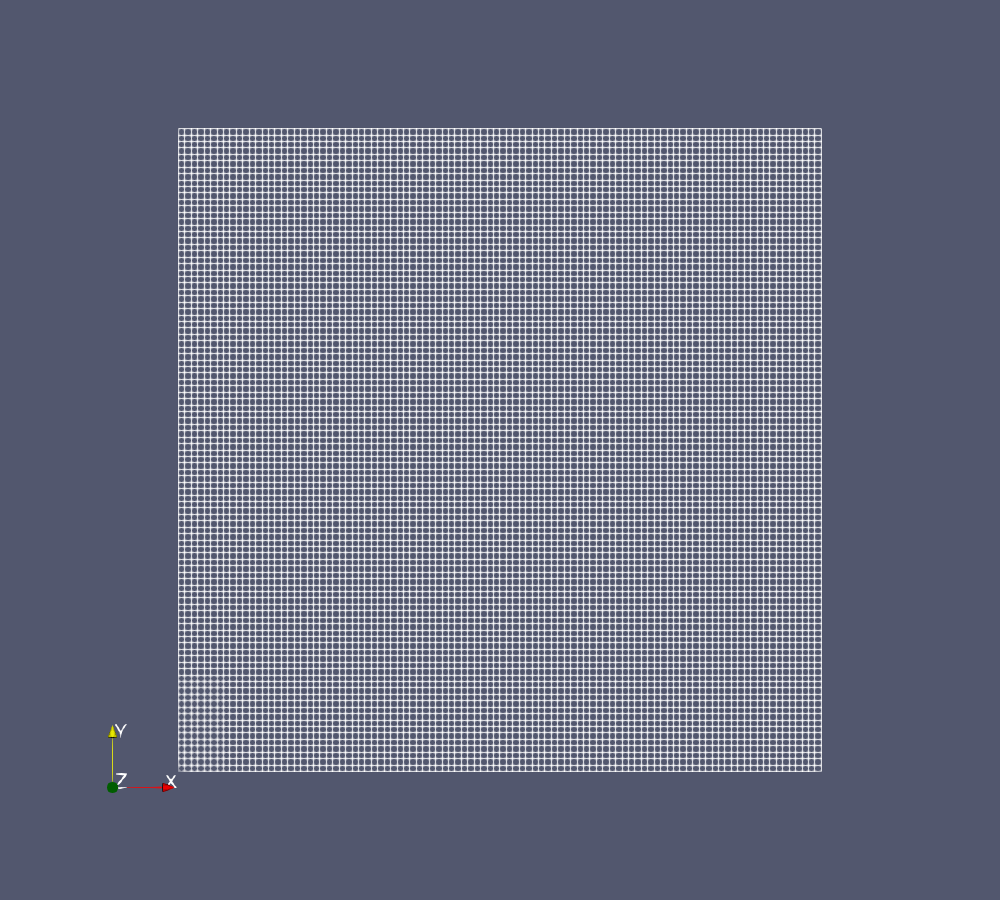
\includegraphics[width=0.6\textwidth]{figures/covo_cedre_mesh.png}
      \caption{Mesh for the isentropic vortex test case with CEDRE.}
      \label{fig:covo_cedre_mesh}
    \end{figure}

    \paragraph{}
    To test the method, we decided to use a simple academic test case, adapted from the one proposed on the International Workshop on High Order CFD Methods (HiOCFD).
    It is a two-dimensional inviscid isentropic vortex that is convected in a periodic box.
    This vortex is an known exact solution of the unsteady Euler equations and is generally considered as a good test case to analyse accuracy of both spatial discretisation and time integration methods.
    It is a non dimensionalised computation, and the mesh is regular over a square of length $L = 20$, with $100^2$ cells.
    It is shown in figure \ref{fig:covo_cedre_mesh}.
    The vortex is convected in a flow at a Mach number of $\operatorname{Ma} = 0.5$, with the dimensioning parameters $P_\infty = 1$ and $T_\infty = 1$.
    The undisturbed velocity is then $U_\infty \vec{e}_x$ with $U_\infty = \operatorname{Ma} \sqrt{\gamma r_\textrm{gas} T_\infty}$ and the vortex is defined using the polar coordinates system $\left(\vec{e}_r, \vec{e}_\theta\right)$:
    \begin{equation}\label{eq:covo}
      \left\{\begin{aligned}
        \vec{u} &= U_\infty \vec{e}_x + \beta U_\infty \frac{r}{R_0} e^{-r^2 / 2 R_0^2} \ \vec{e}_\theta \\[10pt]
        T &= T_\infty - \beta^2 U_\infty^2 \frac{\gamma - 1}{2 \gamma r_\textrm{gas}} e^{-r^2 / R_0^2} \\[10pt]
        P &= P_\infty \left( 1 - \frac{\beta^2 U_\infty^2}{T_\infty} \frac{\gamma - 1}{2 \gamma r_\textrm{gas}} e^{-r^2 / R_0^2} \right)^{\gamma/\left(\gamma - 1\right)} .
      \end{aligned}\right.
    \end{equation}
    The heat capacity ratio $\gamma$ is equal to $1.4$, and the specific gas constant is $r_\textrm{gas} = 1$.
    The vortex is defined by its characteristic radius $R_0 = 1$ and its intensity $\beta = 0.2$.
    This initial condition is shown in figure \ref{fig:covo_cedre_fields}.
    As we solve inviscid Navier--Stokes equations, or Euler equations, the vortex moves in the $\vec{e}_x$ direction undisturbed, and as the domain is periodic the solution after one period $\Delta T = L/U_\infty = 33.8$ is the same as the initial solution.

    \begin{figure}
      \centering
      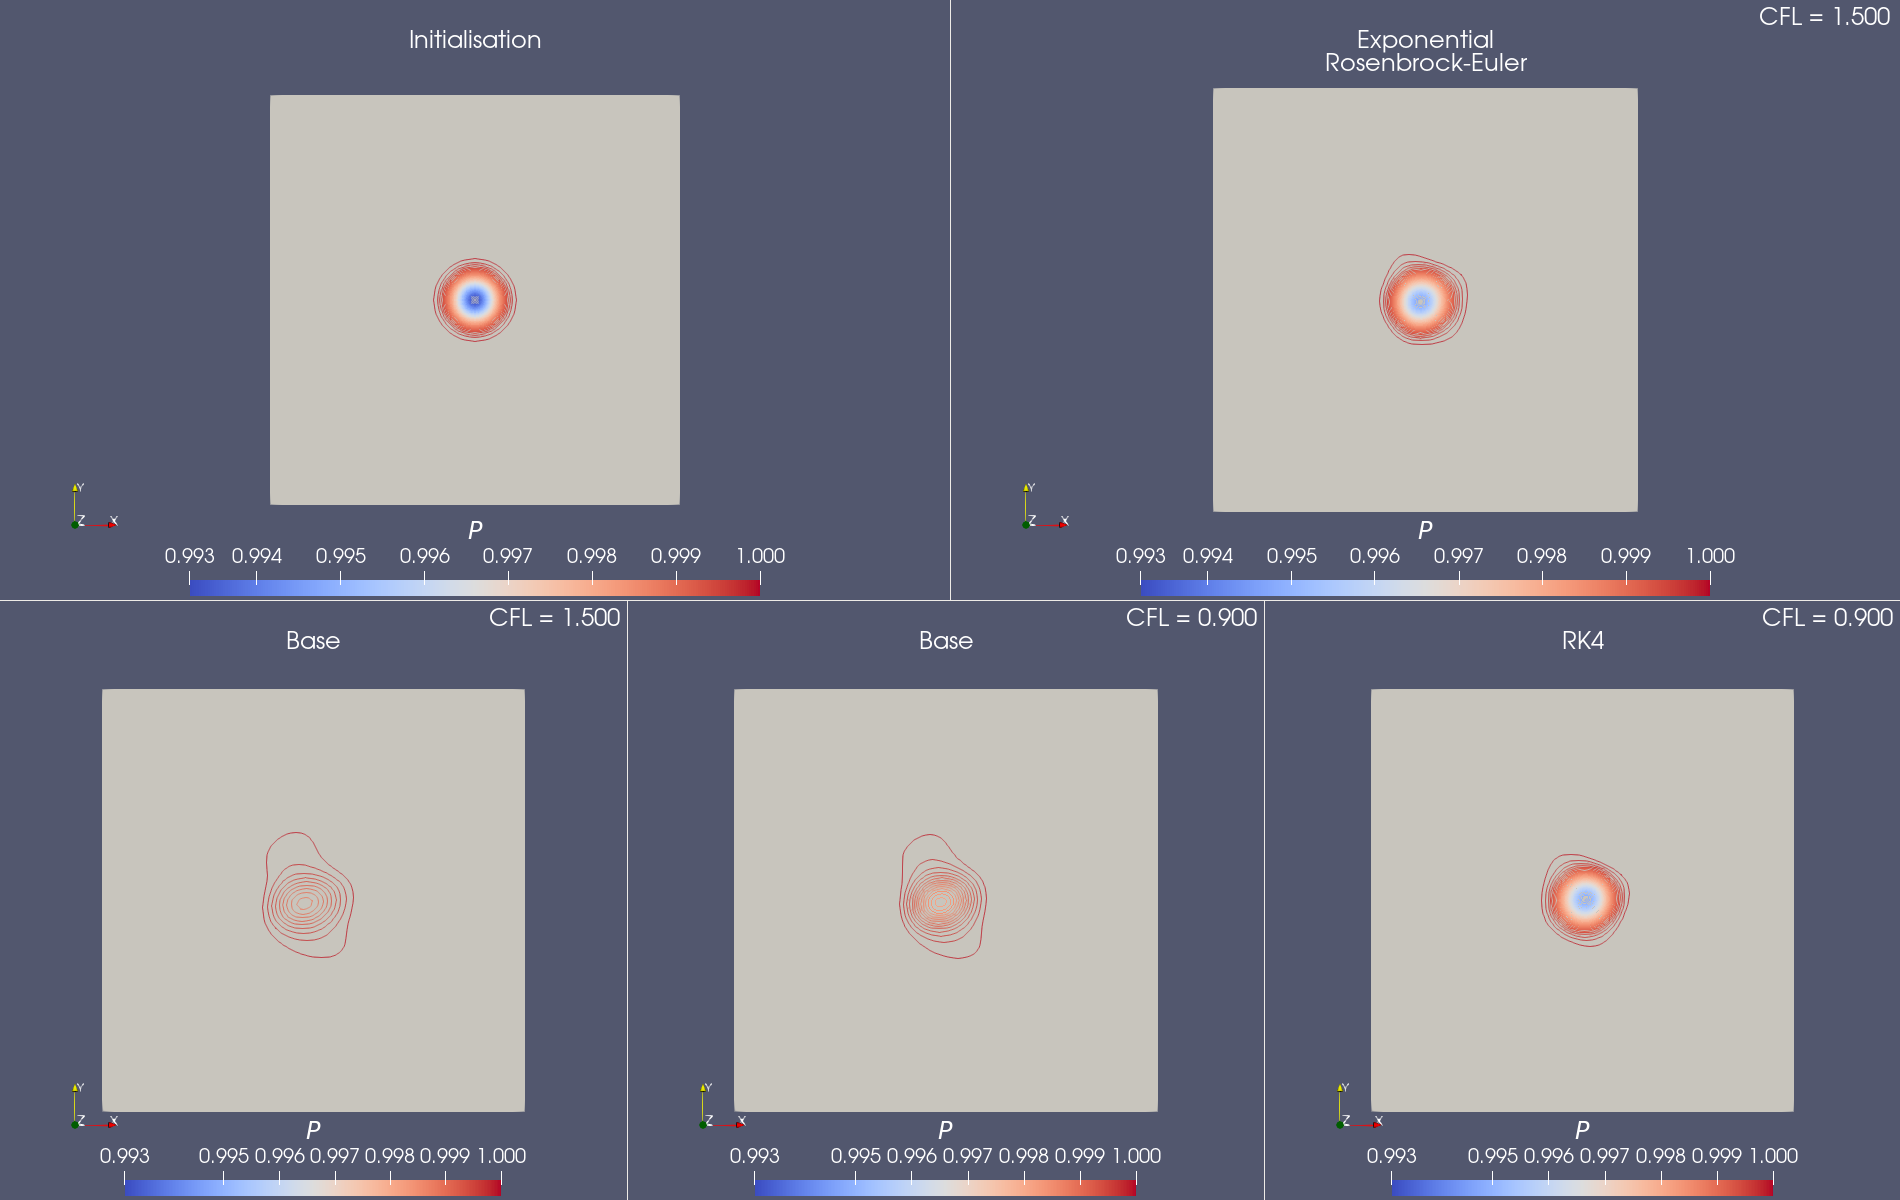
\includegraphics[width=\textwidth]{figures/covo_cedre_fields.png}
      \caption{Initial solution (top left) and solution after one period for the exponential Rosenbrock--Euler method (top right), the implicit Euler method (bottom left and center) and the explicit RK4 method (bottom right).
      The first two simulations correspond to a CFL number of $1.5$ whereas the last two to a CFL number of $0.9$.}
      \label{fig:covo_cedre_fields}
    \end{figure}

    \paragraph{}
    We compare the exponential Rosenbrock--Euler method to the standard implicit Euler method and the classic fourth-order explicit Runge--Kutta method.
    Both the implicit and the exponential methods need to compute Jacobian matrices.
    To reduce the number of variables in this comparison, both will use the traditional Jacobian matrices which is the low-order approximation.
    We then end up with two equivalent methods in terms of computational cost.
    We simulate the vortex advection throughout one period $\Delta T$.
    We show the solution for each method in figure \ref{fig:covo_cedre_fields}.
    We first look at the bottom center and right simulations.
    We see that the explicit Runge--Kutta method preserves well enough the vortex compared to the implicit method.
    It is because the RK4 method is a fourth-order method whereas the implicit method is a first-order method.
    However, the simulations are made at a CFL number of $0.9$.
    With a higher CFL number of $1.5$, the explicit method is unstable and the computation fails.
    The implicit method is able to handle higher CFL numbers, of course as it is the reason implicit methods are used.
    But unsurprisingly we see in the bottom left figure that the solution is even worse.
    Finally, the exponential method is able to handle the higher CFL number and preserve the vortex well enough.
    It has the robustness of the implicit method and the precision of the higher-order explicit method.

    \paragraph{}
    The analysis of this simple test case is quite rudimentary.
    Indeed, we did not look finely at the error introduced by the time integration methods, but we visually compared the results.
    This work showed that at the cost of very few developments we have a method that could prove interesting for time integration with large time steps.
    Its purpose was not to precisely analyse exponential methods but to see their feasibility in our solver.
    Now that this preliminary test showed the quality of exponential time integration methods, we need to perform an actual analysis.

    \paragraph{}
    We see in figure \ref{fig:covo_cedre_fields} that even the methods that preserve the vortex, the exponential and the RK4 methods, do introduce some error.
    Indeed, the vortex after one period is not exactly the same as at the beginning, as it should be.
    We see that it loses in intensity, and the contour lines are not exactly concentric.
    Those symptoms are seen in both computations with the exponential and the higher-order explicit methods.
    Furthermore, the error in the result of those simulations looks similar.
    It is because this error does not come from the time integration method but from the spatial discretisation method.
    Indeed, the spatial discretisation method induces some error when evaluating the right-hand side of equation (\ref{eq:ode_2}).
    This error is accumulated throughout the simulation, and because of it, we could not get the exact result no matter the time integration method.
    What we can do, however, is take a spatial discretisation method such as the error it adds is small compared to the error from the time integration scheme.
    This way, the error we get at the end of the computation is mostly due to the time integration method, and it allows us to compare methods.
    Here the spatial discretisation method used in CEDRE is a second-order method.
    We need to use a higher-order spatial discretisation method to perform the analysis of exponential time integration methods.


    \chapter{Analysis of exponential integration methods in JAGUAR}

\begin{tcolorbox}[title=Résumé du chapitre : Analyse des méthodes d'intégration exponentielles dans JAGUAR, colframe=black!50!white]
  \paragraph{}
  Le but de ce chapitre est de comparer les méthodes exponentielles aux méthodes d'intégration classiques de JAGUAR pour valider leur intérêt.

  \paragraph{}
  Nous avons montré dans le chapitre précédent que CEDRE n'était pas le contexte idéal afin d'analyser des méthodes d'intégration temporelles très précises comme celles qui nous intéressent.
  Nous utilisons donc le solveur JAGUAR, basé sur la méthode des Differences Spectrales, que nous présentons au début de ce chapitre.

  \paragraph{}
  Nous analysons ensuite les méthodes exponentielles ajoutées à JAGUAR grâce à l'utilisation de la librairie SLEPc sur un cas simple, afin de constater l'ordre de ces méthodes à travers l'erreur globale en fin de simulation.
  Sur un autre cas académique, nous comparons ensuite notre ensemble de méthodes en regardant le temps d'exécution qu'il leur est nécessaire afin de réaliser une même simulation.
  Pour finir, nous utilisons les méthodes exponentielles sur un cas plus significatif car proche d'une application réelle du solveur: une aube de turbine.
\end{tcolorbox}

  \paragraph{}
  We want to analyse time exponential integration methods in a framework that gives us access to high-order spatial discretisation methods.
  It is possible to use high-order Finite Volume methods, but this means using larger stencils which hurts parallelism.
  In CEDRE, users often stop at second-order methods, so we need to use another solver.
  As the spatial discretisation method does not play a direct role in the time integration and the work done in this thesis, we can step out from the Finite Volume framework.
  Furthermore, using a less complex solver will also help us try and develop new methods more easily than we already did with CEDRE.
  This is why we decided to accomplish our analysis of exponential time integration methods with the solver JAGUAR.


  \section{JAGUAR: a Spectral Difference solver}

    \paragraph{}
    JAGUAR means proJect of an Aerodynamic solver using General Unstructured grids And high ordeR schemes.
    It is a reactive Navier--Stokes solver originally developed at CERFACS, \PS{the European center for research and advanced training in scientific computing\footnote{je vois pas l'intérêt de le mettre en anglais, soit ça soit j'enlève}}, and is jointly own by ONERA and CERFACS for four years.
    It is made for unstructured grids and uses a Large Eddy Simulation model to solve unsteady turbulence effects.
    It means that the large turbulence scales are computed explicitly while the smaller ones are modelled.
    Its particularity is that it uses a spectral method as spatial discretisation scheme: the Spectral Difference method.
    \PS{The Spectral Difference method follows some principles of the Discontinuous Galerkin formulation, in the sense that both are families of schemes of arbitrary order using polynomial approximations, but their mathematical foundations differ.}


    \subsection{The Spectral Difference method}

      \paragraph{}
      With the Spectral Difference method, the solution is represented by a polynomial of degree $p$ inside each cell.
      It means that in the partial differential equation
      \begin{equation}\label{eq:pde_2}
        \frac{\partial u}{\partial t} + \nabla \cdot F\left(u\right) = 0 ,
      \end{equation}
      $u$ is a $p$-degree polynomial of the coordinate variables, where the polynomial coefficients are functions of time.
      Then $F\left(u\right)$ has to be a $p\!+\!1$-order polynomial of the coordinate variables in order to have a $p$-order polynomial of the flux divergence.
      The key to the Spectral Difference method is how to compute a $p + 1$-order $F\left(u\right)$ from a $p$-order $u$.
      This method uses key elements that were first mentioned by \cite{Kopriva1996}, and were later developed by \cite{LiuVinokurWang2006}.

      \begin{figure}
        \centering
        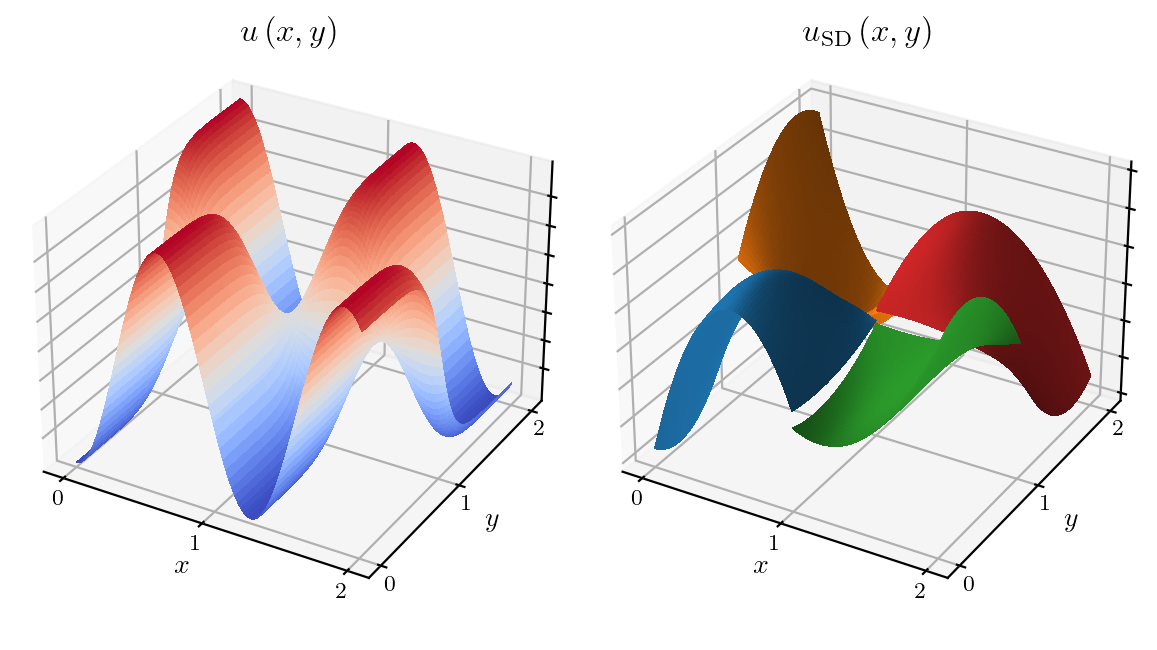
\includegraphics{figures/sd_discontinuous.png}
        \caption{Continuous function (left) and discontinuous representation made by the Spectral Difference method (right).}
        \label{fig:sd_discontinuous}
      \end{figure}

      \paragraph{}
      Because the solution is represented in each cell by a polynomial, there is no reason for the solution to be continuous throughout cell interfaces.
      Indeed, the Spectral Difference method uses a piecewise representation of the solution.
      For example, let us consider the two-dimensional regular mesh, made of $2 \times 2$ cells over $\left[0, 2\right]^2$.
      The exact analytical function $u$ over the mesh in the left part of figure \ref{fig:sd_discontinuous}:
      \begin{equation}
        \begin{aligned}
          u \colon \left[0, 2\right]^2 &\to \mathbb{R}\\
          \left(x, y\right) &\mapsto \cos\left(5x\right) \tanh\left(5\left(1 - y\right)\right)
        \end{aligned}
      \end{equation}
      cannot be represented by polynomial exactly and the right picture of figure \ref{fig:sd_discontinuous} represents the solution associated with the Spectral Difference method.
      The colour mapping corresponds to the output of the function but is not given as this function is of no particular interest: it is a rough example only.
      This function is interpolated with a second-order method using Lagrange polynomials over each cell.
      The result is shown in the right part of figure \ref{fig:sd_discontinuous}, where each colour corresponds to one cell.
      There are discontinuities at the cell interfaces, which shows a specificity of the Spectral Difference methods.
      If the function on the left part of figure \ref{fig:sd_discontinuous} was used as an initial condition for a simulation, the Spectral Difference method would in fact use the polynomial interpolation on the right part.
      However, to respect the underlying conservation property of equation (\ref{eq:pde_2}), it is necessary for $F$ to be continuous over the whole computational domain.
      The Spectral Difference method will then make sure that the polynomial representations of the flux density are continuous throughout cell interfaces.

      \paragraph{}
      To better understand how this method works, let us take a one-dimensional cell: the segment $\left[0, 1\right]$.
      Because the following is done at a fixed time, the dependency on the time is dropped, but the solution and the coefficients are in reality functions of the time, not scalars.
      The solution $u$ inside this segment is then $u\left(x\right) = \sum_{i=0}^p a_ix^i$.
      Using Lagrange interpolation polynomials, it is equivalent to use the set of the $p + 1$ coefficients $a_i$ or the set of the $p + 1$ values $u\left(x_i\right)$ computed at the distinct points $x_i \in \left[0, 1\right]$ called \emph{solution points}.
      The solution as a $p$-order polynomial is represented by either one of those two sets.
      As the flux density $F$ must be a $p\!+\!1$-order polynomial, it can also be represented by its values in the $p + 2$ distinct \emph{flux points}.
      To ensure that $F$ is continuous at the segment end points, we take $0$ and $1$ as flux points.
      The choice of the rest of the flux points will be discussed later, but let us say for now that they are staggered with the solution points: each flux point, apart from the segment end points, is between two solution points and vice versa.

      \begin{figure}
        \centering
        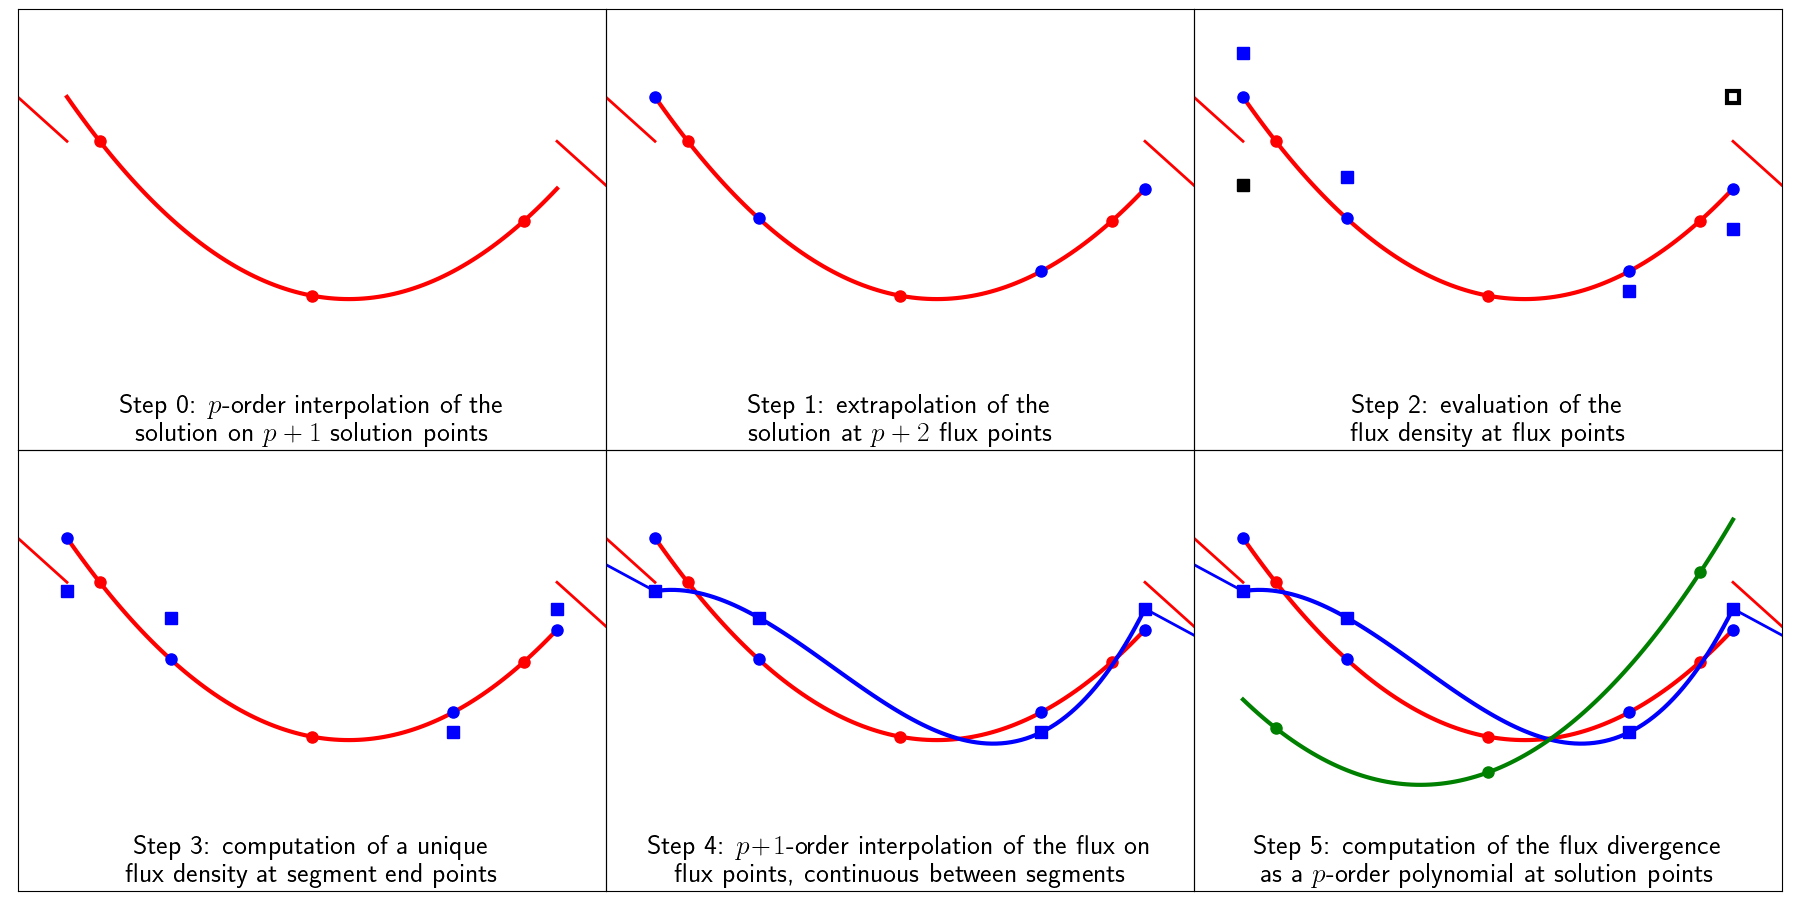
\includegraphics{figures/sd_scheme.png}
        \caption{Steps of the Spectral Difference methods with $p = 2$.}
        \label{fig:sd_scheme}
      \end{figure}

      \paragraph{}
      Figure \ref{fig:sd_scheme} shows the steps the Spectral Difference make to compute the flux divergence $\nabla \cdot F\left(u\right)$ from the solution $u$, with the specific choice $p = 2$.
      \begin{enumerate}
        \setcounter{enumi}{-1}
        \item At first, the solution is represented with a red line by its value in the $p + 1$ solution points.
        The solution points are marked by red dots.
        Parts of the solution from the left and right neighbouring cells can be seen.
        As the figure shows, the piecewise local solutions inside each cell may be discontinuous at the mesh interface.
        This is the starting point of the Spectral Difference method and will be called the 0-th step.
        \item In the first step, the method computes the value of the solution in the $p + 2$ flux points, marked by blue dots.
        As the polynomial representing the solution is known, this step just consists in evaluating it at flux points.
        \item In the second step, the method evaluates the flux density $F\left(u\right)$ in each flux point.
        This is possible because the solution was computed in those points in the previous step.
        The values of the flux density are marked by blue squares in the figure.
        However, segment end points are flux points for the two neighbouring cells, and therefore the figure shows a full black square for the flux at $0$ from the left neighbouring cell and an empty black square for the flux at $1$ from the right neighbouring cell to highlight this discontinuity.
        \item Because there are different values of the flux density at the segment end points, the method would not preserve the conservative property of the partial differential equation.
        This is why in the third step, the method computes a unique interface flux density for both cells at each segment end points.
        The problem is to find the interface flux at the discontinuity of a piecewise solution.
        In other words, this is a Riemann problem.
        Once again, this is solved with a Riemann solver, exact or approximate, to get in the end a single value for the left and right parts of the discontinuity.
        \item An interpolation from the value of the flux density at the $p+2$ flux points using Lagrange polynomials enables to get a $p+1$ order $F$ as expected in the fourth step, represented with a blue line in the figure.
        Therefore, one can end up with a continuous representation of $F$, differentiable everywhere except at cell interfaces.
        \item In the last step, the representation of $F$ is differentiated to get the flux divergence, represented by a green line in the figure.
        Finally, a time integration method can use a $p$-order representation of $\nabla \cdot F$ to compute the solution at the next time step.
      \end{enumerate}

      \paragraph{}
      To work with any segment, not only $\left[0, 1\right]$, an isoparametric transformation is introduced to get back to this unity segment.
      It is the same when working with multiple dimensions, where the isoparametric transformation gets the cell back to the tensor powers of this segment.
      The placement of the solution points does not seem to matter much, but the placement of the flux points does \cite{VandenAbeeleLacorWang2008}.
      The $p + 1$ solution points we will use are defined in the $\left[0, 1\right]$ segment as the Chebyshev roots:
      \begin{equation}
        x_i = \frac{1}{2} \left(1 - \cos\left(\frac{2i + 1}{2p + 2} \pi\right)\right), \quad 0 \leq i \leq p .
      \end{equation}
      They are traditionally defined inside the $\left[-1, 1\right]$ segment but are scaled into $\left[0, 1\right]$.
      They are the roots of the Chebyshev polynomials of the first kind and are often used in polynomial interpolation as they tend to minimise Runge's phenomenon.
      The $p + 2$ flux points are the $p$ roots of the $p$-th Legendre polynomials to which are added the two segment end points.
      This choice has the property that there is a flux point between each contiguous solution point.
      There is no explicit formula for the Legendre polynomial roots as there is one for the Chebyshev polynomial roots.
      They are also defined in the $\left[-1, 1\right]$ segment and are scaled into $\left[0, 1\right]$.
      Finally, the solution and flux points can be seen in figure \ref{fig:sd_points}.

      \begin{figure}
        \centering
        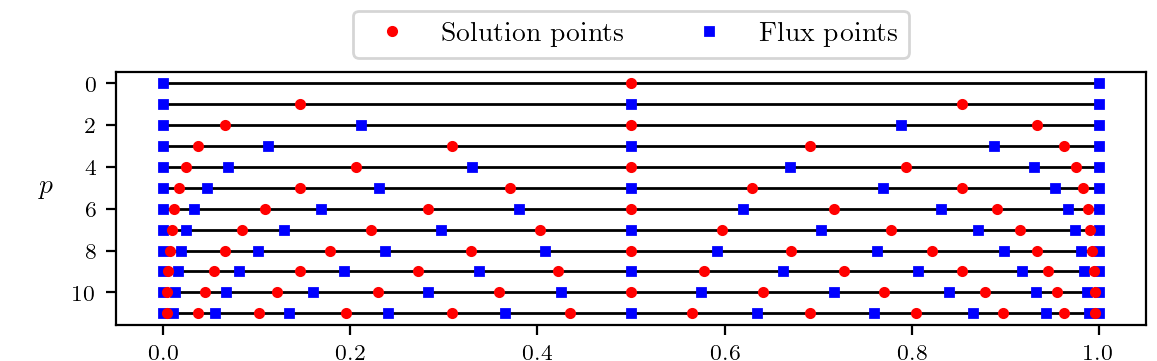
\includegraphics{figures/sd_points.png}
        \caption{Solution points and flux points in the $\left[0, 1\right]$ segment used in the Spectral Difference method for $0 \leq p \leq 11$.}
        \label{fig:sd_points}
      \end{figure}

      \paragraph{}
      As a side note, the Spectral Difference method with $p = 0$ corresponds roughly\footnote{\PS{Pourquoi roughly?}} to the first-order Finite Volume method.
      Indeed, the solution is assumed constant in the cell, represented by the value at its barycenter.
      The flux balance is made at the cell interfaces with a Riemann solver.
      This corresponds to the placement of the solution and flux points in figure \ref{fig:sd_points} when $p = 0$.
      For higher $p$, the proposed Spectral Difference method is naturally of order $p$
      Indeed, the method can represent exactly any polynomial of degree $p\!-\!1$ and, as a consequence, the error term is of order $p$.
      In JAGUAR, the order $p$ range from 2 to 10, but $2 \le p \le 6$ for practical applications.

      \paragraph{}
      The demonstration of the accuracy of the Spectral Difference method is proposed in a reference paper published recently \cite{VanharenPuigtVasseurEtAl2017}.
      JAGUAR was optimised to be efficient for parallel computations \cite{Cassagne2014, CassagnePuigtBoussuge2015, Marait2015}.
      To perform Large Eddy Simulation, it is of paramount importance to implement unsteady characteristic boundary condition: Navier--Stokes Characteristic Boundary Condition, or NSCBC.
      The initial formulation \cite{FievetDeniauPiot2020} was extended to deal with acoustic conditions and liner optimisation \cite{CardesaFievetPiotEtAl2022}.
      Recently, the solver was extended to handle $h-p$ adaptation \cite{HartmannBalanBassiEtAl2021} and the schemes were extended to triangles and tetrahedrons \cite{VeilleuxPuigtDeniauEtAl2022, VeilleuxPuigtDeniauEtAl2022a}.
      Another improvement concerns the treatment of combustion, with a PhD thesis funded by Safran \cite{MarchalDeniauBoussugeEtAl2021}.
      Finally, the last extension concerns the treatment of shocks \cite{DeniauPuigt2022}.
      This review shows the strong involvement of researchers on the solver.


    \subsection{Exponential integration methods in JAGUAR}

      \paragraph{}
      Using a high-order spatial discretisation method and a refined mesh is the best suited situation to test high-order time integration methods: the resulting error will come mostly from the time integration and not the spatial discretisation.
      The development of an exponential time integration method was inexpensive within CEDRE as the method reuses lots of already existing parts.
      For JAGUAR which only has explicit methods, the Arnoldi iteration and the exponential computation functions must be implemented to use exponential methods.
      They could be developed as internal stand-alone routines to produce a finely tuned method for JAGUAR.
      However, since the goal is to analyse exponential methods scientifically, it was decided to rely on the SLEPc library \cite{HernandezRomanVidal2005}.
      The Scalable Library for Eigenvalue Problem Computation, or SLEPc, is an extension of the software library PETSc \cite{petsc-web-page, petsc-user-ref, petsc-efficient}.
      Instead of rewriting the needed algorithms, it was chosen to use their SLEPc implementation.
      In particular, SLEPc handles what it calls \emph{Matrix Function} objects or MFN:
      \begin{quote}
        "Given a matrix $A$ and a vector $b$, the call \mintinline{c}{MFNSolve(mfn, b, x)} computes \\
        $x=f\left(A\right) b$, where $f$ is a function such as the exponential."
      \end{quote}
      This is precisely what is needed to develop exponential methods: as it handles the previously introduced $\varphi$-functions with its MFN objects, SLEPc is then an obvious choice of a library for implementing exponential integration methods.
      Furthermore, because it relies on PETSc, it is efficiently scalable to fit our multiprocessing needs.

      \paragraph{}
      Exponential methods are based on a decomposition of the ordinary differential equation such as equation (\ref{eq:ode_split}).
      However, JAGUAR uses only explicit time integration methods, so no Jacobian matrix is available.
      Computing analytically the Jacobian matrix would prove challenging as any ingredient should be differentiated, such as the Spectral Difference scheme, the Riemann solvers, the diffusion scheme, etc.
      It is not insurmountable but would amount to more work than what could be afforded during this thesis.
      It was decided instead to reuse the work from the previous part: the Jacobian matrix will not be formed, but its effect will be computed by a finite difference approximation.
      Another reason to work with the SLEPc library is that using a finite difference approximation is easy with it.
      More precisely, it is PETSc that handles this approximation.
      \PS{To sum up, to compute $\varphi_k\left(L\right)b$ that is required for the exponential methods with $L = f'\left(y\right)$, $L$ is created with the appropriate PETSc data type.
      As it is a Jacobian matrix of a function, PETSc only needs to know the function to compute matrix-vector products.}
      Then, after setting the MFN object of SLEPc, the library can compute the desired result
      The Arnoldi iteration, the Scaling and Squaring algorithm and the exponential evaluation are all handled internally by the library.
      Overall, this procedure is extremely simple from our perspective and requires only a few lines of code to implement.
      This highlights the relevance of using the SLEPc library to easily test procedures and acquire the associated knowledge.

      \paragraph{}
      Other people that also work with JAGUAR did develop implicit time integration methods using PETSc.
      To continue in this direction, it was decided to add a time integration method based on the generic PETSc Time Stepper \cite{AbhyankarBrownConstantinescuEtAl2018}.
      This way, a user may use most methods from PETSc in JAGUAR with no additional developments.
      It includes any explicit and implicit time integration methods, but also nonlinear solvers such as Newton's methods with various line search algorithms, linear solvers with various Krylov subspace methods and finally various preconditioning.
      However, this generic PETSc Time Stepper method was added on the side of this thesis, and therefore will not be discussed here, along with the previous work on implicit methods.


    \paragraph{}
    In the end, the high-order spatial discretisation method called the Spectral Difference method allows to analyse and compare exponential methods that are available through the SLEPc library.
    In the following, attention is mainly focused on the three methods that were presented earlier in table \ref{tab:exprb_butcher}: the Rosenbrock--Euler, ExpRB32 and ExpRB42 methods.


  \section{Analysis of exponential time integration methods}

    \paragraph{}
    There are in JAGUAR all the tools necessary to analyse exponential time integration methods and several test case must be chosen.
    During the analysis, the exponential methods and explicit Runge--Kutta methods will be compared, as the latest ones are the only available methods in JAGUAR and represent the state-of-the-art.
    Those methods are:
    \begin{itemize}
      \item RK2, the Midpoint method
      \item RK4, the classical four-stage fourth-order method
      \item RKo6s, a low-storage, low-dissipation and low-dispersion six-stage second-order method from \cite{BogeyBailly2004} dedicated to unsteady computations
      \item TVDRK(3, 3), a three-stage third-order TVD method from \cite{ShuOsher1988, GottliebShu1996}
      \item SSPRK(5, 4), an optimal SSP five-stage fourth-order method from \cite{SpiteriRuuth2002}.
    \end{itemize}
    Low-storage methods are Runge--Kutta methods for which the matrix $A$ in their Butcher tableau is lower diagonal, or in other words all $a_{ij}$ are null except when $j = i - 1$.
    Also, all $b_i$ are null except the last one that is equal to $1$.
    It means that the final stage and all intermediate ones use only the previous stage.
    Therefore, there is no need to keep track of intermediate stages in memory, only to update the current value, which gives the name low-storage method.
    The last two methods are Runge--Kutta methods with an additional property originally called TVD \cite{GottliebShu1996} and more recently SSP  \cite{GottliebShuTadmor2001}.
    Without going into too much detail, it means that they are methods that are convex combinations of explicit Euler steps so that their stability is guaranteed for sufficiently small time steps.
    To us, it means they are defined differently than other methods, using the coefficients $\alpha_{0 < i \leq k, 0\leq j < i}$ and $\beta_{0 < i \leq k, 0\leq j < i}$ as:
    \begin{equation}
      \left\{\begin{aligned}
        y_{n+1} &= y^{\left(k\right)} \\
        \textrm{with}\quad y^{\left(i\right)} &= \sum_{j = 0}^{i-1} \alpha_{ij} y^{\left(j\right)} + \Delta t \beta_{ij} f\left(y^{\left(j\right)}\right) , \quad 1 \leq i \leq k\\
        \textrm{and}\quad y^{\left(0\right)} &= y_n
      \end{aligned}\right. .
    \end{equation}
    However, they are equivalent to traditional Runge--Kutta methods in the sense that they can be represented by the standard Butcher tableau, with:
    \begin{equation}
      \left\{\begin{aligned}
        a_{ij} &= \sum_{l = j+1}^{i-1} \alpha_{i-1, l-1} a_{l, j} + \beta_{i-1, j-1} \\
        b_i &= \sum_{l = i+1}^{k} \alpha_{k, l-1} a_{l, i} + \beta_{k, i-1}
      \end{aligned}\right. .
    \end{equation}
    We can finally say that we are indeed working with explicit Runge--Kutta methods, as they were introduced initially.


    \subsection{Order analysis: convected inviscid isentropic vortex}

      \paragraph{}
      This first case is designed to analyse the order of accuracy of the proposed methods and to validate their implementation.
      Is is the simple case of the two-dimensional inviscid isentropic vortex, the same as the one considered with CEDRE.
      The case is still described by equation \ref{eq:covo}, but the numerical values are different.
      The convective flow Mach number is still $0.5$, but this time $P_\infty = 10^5\si{\pascal}$ and $T_\infty = 300\si{\kelvin}$.
      The heat capacity ratio is $\gamma = 1.4$ and the specific gas constant is $r_\textrm{gas} = 287.058\si{\joule\per\kilo\gram\per\kelvin}$.
      Those values correspond to standard values for dry air.
      The mesh represent the two-dimensional box $\left[0, L\right]^2$ with $L = 0.1\si{\meter}$, and is made of $N \times N$ cells.
      The vortex is defined by its characteristic radius $R_0 = 0.005\si{\meter}$ and its intensity $\beta = 0.2$.
      It corresponds in fact to the same vortex as the one used with CEDRE, in size and in intensity, but it has been scaled down into a smaller box and dimensioned to some given pressure and temperature.
      The present choice is in agreement with the prescription of the International Workshop on High Order CFD Methods.

      \paragraph{}
      \GP{Quel solveur de Riemann ???? Tu ne l'as pas dit...}
      \PS{Comment ça ?}

      \paragraph{}
      The period for those numerical values is $L / U_\infty = \num{0.0005759974000734113}\si{\second}$.
      After 20 periods, the vortex should recover the initial position and the 2-norm of the error between initial and computed solutions can be defined for any scalar variable $u\left(\vec{x}, t\right)$:
      \begin{equation}
        \operatorname{err}\left(u\right) = \left(\int_{\left[0, L\right]^2} \left(u\left(\vec{x}, 20T\right) - u\left(\vec{x}, 0\right)\right)^2 \mathrm{d}\vec{x} \right)^{1/2} .
      \end{equation}
      \PS{
      %\GP{ Je vire ca car c'est pas tout à fait vrai... Because it is a periodic case, the initial value corresponds to the exact solution.
      %This error corresponds then to the error of the time integration method.}\\
      %Je mets ça à la place:
      Once the vortex moves in the domain, the numerical solution is subject to two schemes and errors are a consequence of both.
      Once the spatial scheme is defined, the mesh is chosen sufficiently refined in order to transport the vortex accurately and the goal is to have a much lower influence of the spatial scheme than of the time integration scheme on the total error.
      The order of our time integration methods can be determined by looking at this error as a function of the time step.
      }

      \paragraph{}
      The error at the end of the simulation is the global truncation error: the error the method makes while getting to a fixed time, no matter how many iterations it took.
      However, the order of a time integration method was previously defined using the local truncation error: the error it makes after a single small step.
      There is a link between global and local truncation errors for our single-step methods.
      Let us call $\tau_n$ the local truncation error and $e_n$ the global truncation error at step $n$.
      Because single-step methods can be written as:
      \begin{equation}
        y_{n+1} = y_n + \Delta t_n g\left(y_n, \Delta t_n\right) ,
      \end{equation}
      with an increment function $g$ that is $K$-Lipschitz continuous in the $y$ variable, the global truncation error is bounded \cite{SueliMayers2003}:
      \begin{equation}
        \left| e_n \right| \leq \frac{\max_{1 \leq i \leq n} \left| \tau_i \right|}{K \Delta t_n} \left(e^{K\left(t_n - t_0\right)} - 1\right) .
      \end{equation}
      A method is a $p$-order method if $\tau_n = O\left(\Delta t^{p+1}\right)$.
      Therefore, a $p$-order method verify $e_n = O\left(\Delta t^{p}\right)$.
      However, the reciprocal is not true: observing a global truncation error $e_n = O\left(\Delta t^{p}\right)$ does not mean the order of the method is $p$.
      As a consequence, attention is focused on the expected order for the global truncation error at the end of the computation, as it is the error users look at.
      The proof of the order for a method is analytical, by writing the partial Taylor series of the exact solution, as we did earlier for the exponential Rosenbrock--Euler method.

      \paragraph{}
      The point of this analysis is to see how the global truncation error depends on the time step $\Delta t$ that is kept constant throughout the computations.
      Because some methods are more accurate than others, several computations with different mesh resolutions and Spectral Difference method orders were made.
      Let us start with the Midpoint method, associated with the order of the spatial discretisation method $p = 4$. The computation is stopped after 20 periods and the $L_2$ error for the pressure is analysed for different time steps.
      Results are shown using the CFL number as it is proportional to the time step:
      \begin{equation}
        \mathcal{N}_\textrm{CFL} = \frac{N \left(p + 1\right) \left(1 + \operatorname{Ma}\right) \sqrt{\gamma r_\textrm{gas} T}}{L} \Delta t .
      \end{equation}
      Using the CFL number instead of the time step allows to compare results with different $N$ or even $p$.
      It can be seen here as a nondimensional time.
      Computations are made for multiple values of $N$: 16, 32 and 64, and the corresponding results are shown in figure \ref{fig:covo_rk2}.
      The $16\times16$ mesh does not allow for a good analysis: the error due to the spatial discretisation method is too important and prevents to see the expected dependency between the global truncation error and the time step.
      The two other meshes however show the expected relation: $\operatorname{err} = O\left(\Delta t^2\right)$.

      \begin{figure}
        \centering
        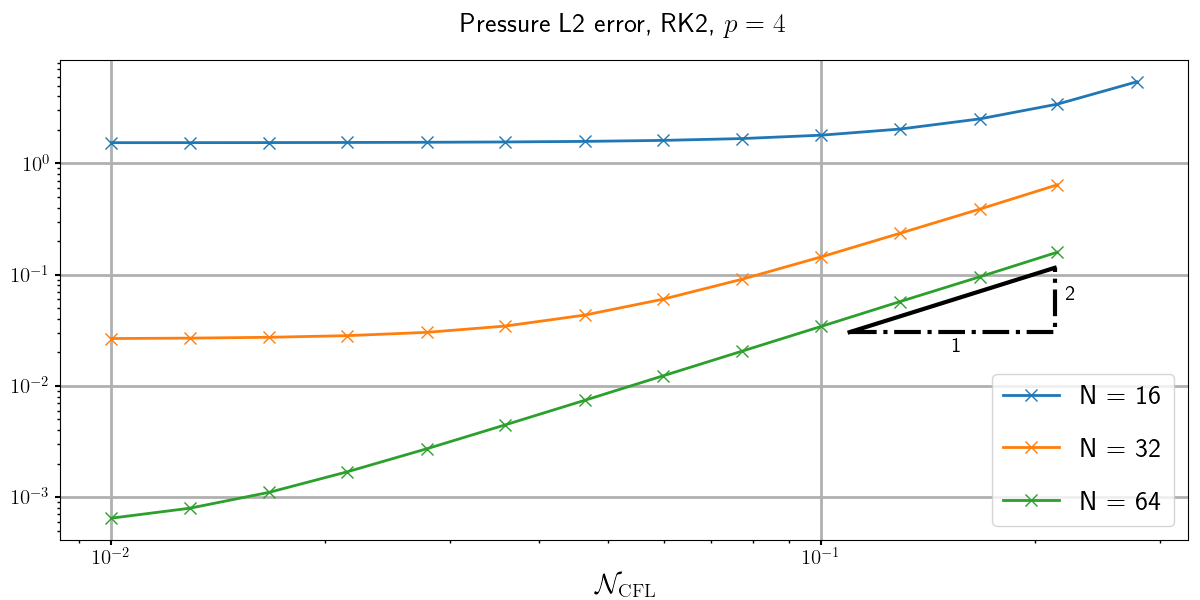
\includegraphics{figures/covo_rk2.png}
        \caption{Global truncation error for the RK2 Midpoint method.}
        \label{fig:covo_rk2}
      \end{figure}

      \paragraph{}
      This analysis is repeated for other methods, and we look now at the RK4 method.
      However, figure \ref{fig:covo_rk2_rk4} shows that the error is constant no matter the value of $N$.
      It is because the error due to the RK4 method is so small that it is dominated by the error due to the spatial discretisation scheme.
      It is useless to do the same for lower time steps, as the error would not change, therefore the RK4 error lines are continued by black dashed lines.
      As the time step decreases, the curves from the Midpoint scheme tend to the same dashed lines: this is the proof that this lower bound for the error corresponds to the error of the spatial discretisation method.
      It shows once again that a spatial discretisation method with small errors is necessary in order to analyse time integration methods.

      \begin{figure}
        \centering
        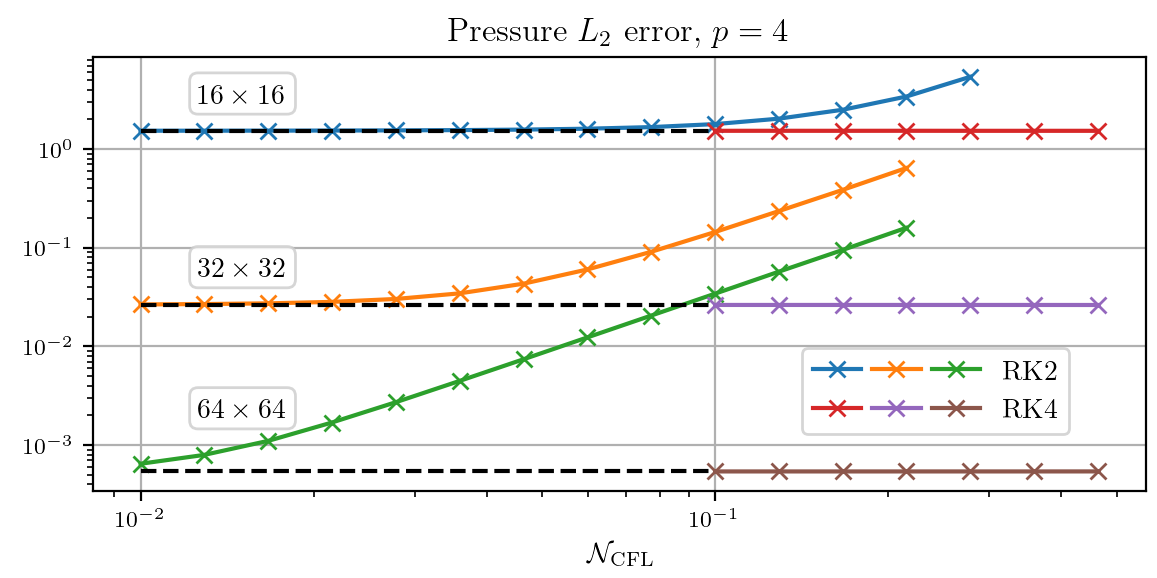
\includegraphics{figures/covo_rk2_rk4.png}
        \caption{Global truncation error for the RK2 and RK4 method.}
        \label{fig:covo_rk2_rk4}
      \end{figure}

      \paragraph{}
      Increasing $N$ up to 128 and then 256 was unsuccessful: the error was still constant.
      Instead of refining the mesh, an analysis playing with the Spectral Difference method can be performed by increasing the spatial discretisation order.
      As the theory behind this analysis does not directly depend on $N$ and $p$, we can adjust them to better fit the method we want to analyse.
      This is done in figure \ref{fig:covo_rk} where the global truncation error is shown as a function of the time step, or CFL number, for the RK4, RKo6s and TVDRK(3, 3) methods.
      The expected slopes for the second and third-order methods are obtained but the result is more subtle for the fourth-order method.
      The error is once again dominated by the error of the spatial discretisation scheme.
      On the right part of the curve, one can guess the correct slope but it is necessary to plot the error for larger time step values
      to see it more clearly.
      However, those larger time step values are outside the stability domain of the method.
      In fact, all curves end on the right at the largest time step for which the computation did not fail.
      It means from figure \ref{fig:covo_rk} that the RKo6s method is more stable than both the RK4 and TVDRK(3, 3) methods.
      This is the issue with this analysis: for too small time steps, the error from the spatial discretisation method is dominant and the expected slope are not recovered.
      On the other hand, with too large time steps, computations fall outside the stability region of the method.
      The difficulty is to find the correct window that allows to observe the desired slope by choosing suitable values for $p$ and $N$.
      Because the error of the SSPRK(5, 4) is particularly small, it was not possible to find reasonable values below $p = 8$ and $N = 64$.
      Above those values, the computations get rather long so we skipped this method.

      \begin{figure}
        \centering
        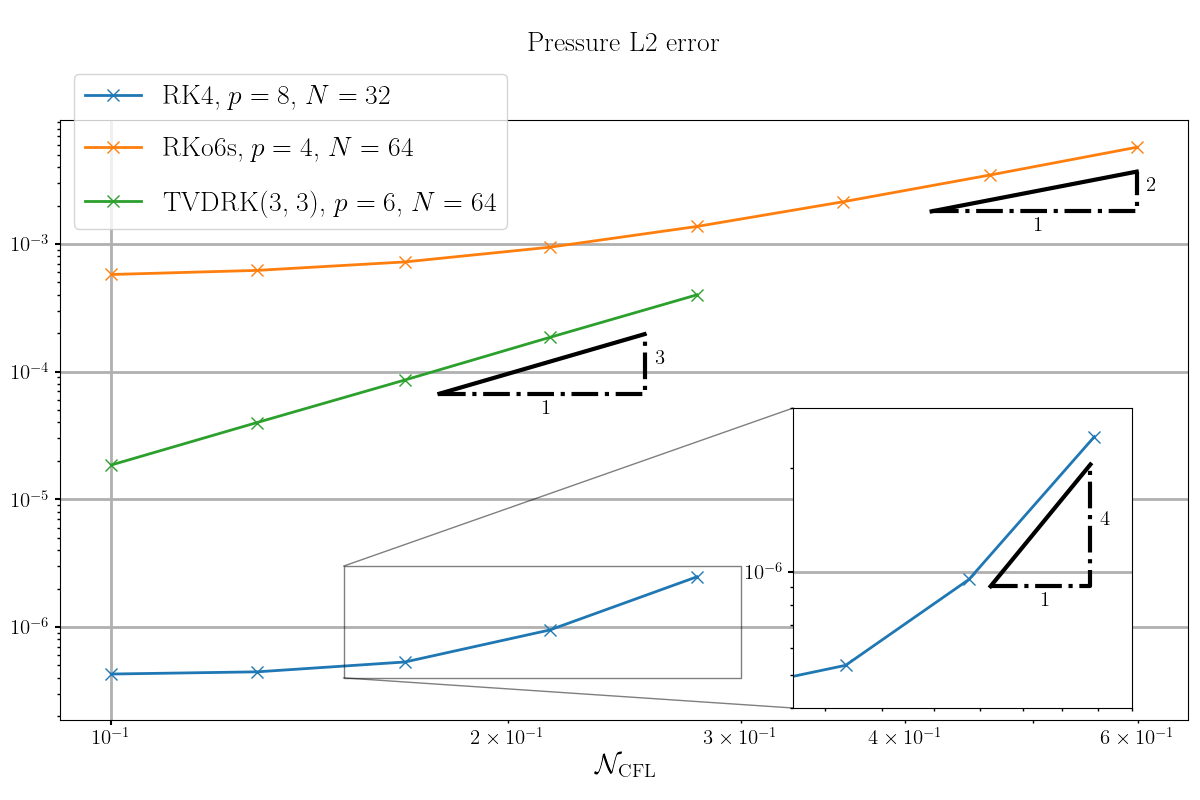
\includegraphics{figures/covo_rk.png}
        \caption{Global truncation error for the RK4, RKo6s and TVDRK(3, 3) methods.}
        \label{fig:covo_rk}
      \end{figure}

      \paragraph{}
      The analysis on traditional explicit Runge--Kutta methods can now be applied to the newly added exponential Rosenbrock methods.
      Their corresponding error curves are shown in figure \ref{fig:covo_exp}.
      As expected, the respective slope values are 2, 3 and 4.
      Furthermore, by looking at the abscissa ranges, they work correctly with higher CFL numbers than all the explicit methods that were tested.
      The goal of this first analysis of the exponential integration methods is not to analyse their robustness, but it already seems better than with explicit methods.
      What is interesting from this analysis is that one can use higher-order methods with fewer Runge--Kutta stages.
      Furthermore, the additional computational cost of the additional stages is low.
      As discussed earlier, exponential Rosenbrock methods can be reformulated as in equation (\ref{eq:exprb_defect}) using the defects $D_{n, i}$.
      The first stage of an exponential Rosenbrock method is then an exponential Rosenbrock--Euler method, for which the contribution of the "full" right-hand side $f\left(y_n\right)$ is used.
      Here, this is done with the algorithms previously described, using a Krylov subspace of dimension 20.
      Then, because the defects are relatively smaller, the other stages compute their contribution with only 5 Krylov basis vectors.
      The two exponential Rosenbrock methods with two stages are not a lot more expensive than the Rosenbrock--Euler method.
      In comparison, a 2-stage explicit Runge--Kutta method will be twice as computationally expensive as the Euler method.
      This analysis was also performed with larger Krylov subspace methods.
      In this other configuration, the first stage uses 40 Krylov basis vectors for all three exponential methods, and the second stage uses 10 Krylov basis vectors for the ExpRB32 and ExpRB42 methods.
      However, using a larger subspace did not have any impact on the result of this analysis.
      For all $\left(N, p\right)$ configurations, the error curve as a function of the time step was almost the same as with smaller Krylov subspace, such as they were almost indistinguishable when plotted in figures like figure \ref{fig:covo_exp}.

      \begin{figure}
        \centering
        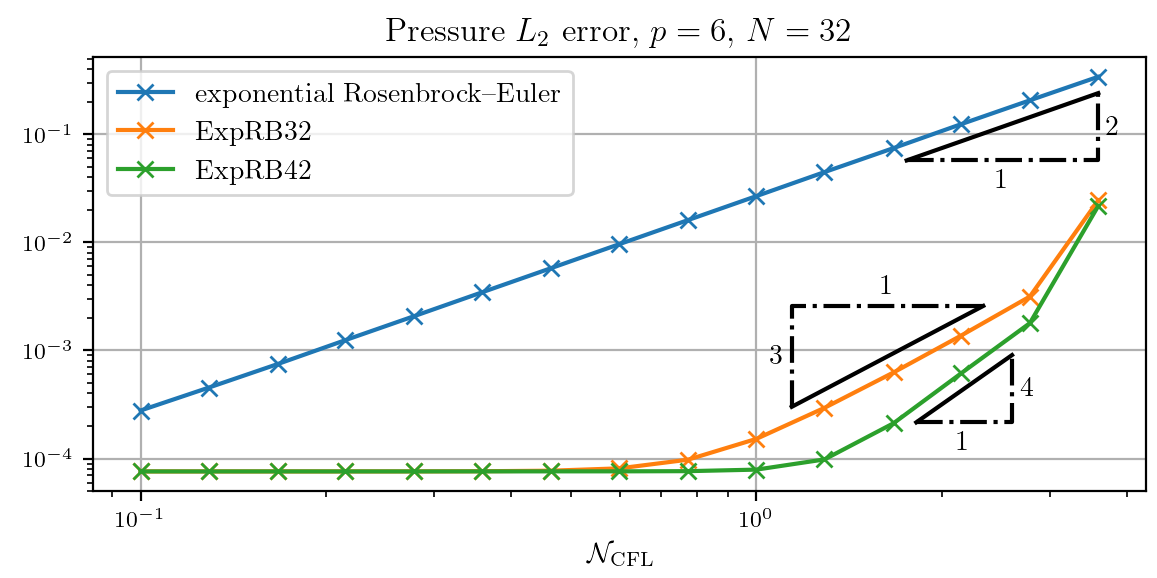
\includegraphics{figures/covo_exp.png}
        \caption{Global truncation error for the exponential Rosenbrock--Euler, ExpRB32 and ExpRB42 methods.}
        \label{fig:covo_exp}
      \end{figure}

      \paragraph{}
      We choose this first test case as it is widespread in the computational fluid dynamic community, as a tool to analyse the order of integration schemes.
      It often concerns spatial discretisation methods, but it can be considered for time integration method as it gives access to the global truncation error, which is the error that interests the solver users.
      First, this analysis recovers the correct slope on the error curve as a function of the time step for the already existing explicit Runge--Kutta integration methods.
      Indeed, the error converges, as the time step decreases, to a minimum error value that comes from the spatial discretisation scheme.
      By refining the mesh and using higher-order spatial discretisation methods, we are able to reduce this minimal error and observe the expected curve for almost all methods.
      The same analysis but with the newly implemented exponential Rosenbrock methods showed the expected order.
      It also showed that the additional cost of using more stages with exponential methods is relatively small compared to the same additional cost for explicit Runge--Kutta methods.
      Finally, for this convected inviscid isentropic vortex case, the exponential Rosenbrock methods were much more robust, as they work with higher CFL numbers.
      The analysis of their stability is the topic of the next section.


    \subsection{Robustness analysis: Taylor--Green vortex}

      \paragraph{}
      The Taylor--Green vortex consists in following the evolution of a set of vortices in a periodic domain.
      It is a three-dimensional case, solution of the Navier--Stokes equations in a periodic box of length $2 \pi L$ centered around the origin.
      The initial flow is given by:
      \begin{equation}\label{eq:tgv}
        \left\{\begin{aligned}
          \vec{u} &= \operatorname{Ma} \sqrt{\gamma r_\textrm{gas} T_\infty} \begin{pmatrix}
            \sin\left(\frac{x}{L}\right) \cos\left(\frac{y}{L}\right) \cos\left(\frac{z}{L}\right) \\[10pt]
            \cos\left(\frac{x}{L}\right) \sin\left(\frac{y}{L}\right) \cos\left(\frac{z}{L}\right) \\[10pt]
            0
          \end{pmatrix} \\[10pt]
          T &= T_\infty \\[10pt]
          P &= P_\infty \left(1 + \frac{\gamma \operatorname{Ma}^2}{16} \left(\cos\left(\frac{2x}{L}\right) + \cos\left(\frac{2y}{L}\right)\right) \left(\cos\left(\frac{2z}{L}\right) + 2\right) \right)
        \end{aligned}\right.
      \end{equation}
      over the domain $\left(x, y, z\right) \in \left[-\pi L, \pi L\right]^3$, as seen in figure \ref{fig:tgv_fields}.
      Even if $\vec{u}_z = 0$ at the initialisation, it becomes non-null afterwards and the problem is fully three-dimensional.
      The initial flow transition to turbulence: the initial large scales decay into smaller ones, that end up dissipated.

      \begin{figure}
        \centering
        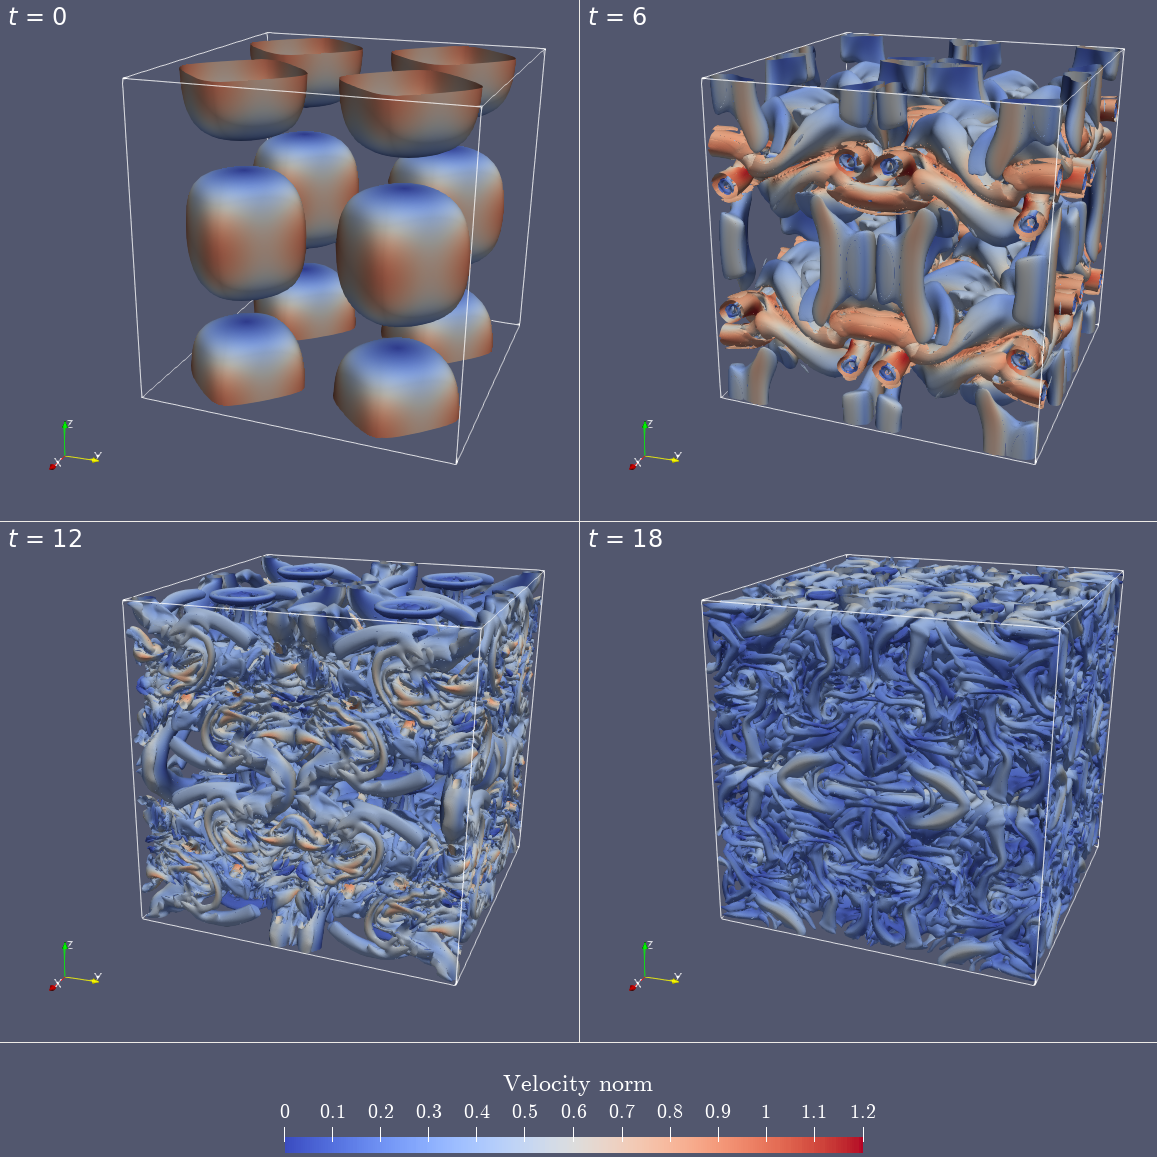
\includegraphics[width=\textwidth]{figures/tgv_fields.png}
        \caption{\PS{TODO}}
        \label{fig:tgv_fields}
      \end{figure}

      \paragraph{}
      The numerical values are non dimensionalised: $L = 1$, $\operatorname{Ma} = 0.1$, $r_\textrm{gas} = 71.4284$, $T_\infty = 1$ and $P_\infty = 71.4288$.
      The goal is to recover the Reynolds number $\operatorname{Re} = \rho_\infty U\infty L / \mu = 1600$ with the associated constant fluid viscosity is $\mu = \num{6.25e-4}$.
      The Prandtl number, ratio of momentum diffusivity to thermal diffusivity, is equal to 0.71.
      Using the convective time $t_c = L / U_\infty$, it is known that the maximum of dissipation happens around $8 t_c$, and after $15 t_c$ the flow is fully turbulent without any trace of the initial structures.
      The definition of the test case is part of the International Workshop on High-Order CFD Methods.
      A reference solution is also provided by the workshop, obtained using a spectral solver on a very refined mesh.

      \paragraph{}
      The values of interest for this test case are the temporal evolution of the mean turbulent kinetic energy over the computational domain $\Omega$:
      \begin{equation}
        E_k = \frac{1}{\rho_\infty \left|\Omega\right|} \int_\Omega \rho \frac{\norm{\vec{u}}^2}{2} \mathrm{d}\Omega ,
      \end{equation}
      the mean enstrophy, defined by
      \begin{equation}
        \mathcal{E} = \frac{1}{\rho_\infty \left|\Omega\right|} \int_\Omega \rho \frac{\norm{\nabla \times \vec{u}}^2}{2} \mathrm{d}\Omega ,
      \end{equation}
      and the kinetic energy dissipation rate, that follows the relation \PS{MAIS EN FAIT JE LA MONTRE PAS}:
      \begin{equation}
        \epsilon = -\frac{\mathrm{d} E_k}{\mathrm{d} t} = 2 \mu \mathcal{E} .
      \end{equation}
      Those values computed by the present simulation are compared with the reference values.

      \paragraph{}
      The mesh used here is the same for all computations: a regular Cartesian mesh made of $80^3$ cells.
      This choice is not natural from the workshop but previous experiments have lead to the conclusion that such a mesh gives the best solution at the lowest CPU cost, for the Spectral Difference method with the order $p = 4$.
      Each computation is run on 308 CPU cores.
      The goal is to see if the result from the simulation matches reference data up to $20 t_c$, and how much CPU time the computation took.
      The RKo6s, TVDRK(3, 3) and SSPRK(5, 4) methods are the already existing reference methods, and the exponential Rosenbrock--Euler, ExpRB32 and ExpRB42 methods are the newly implemented methods.
      For the exponential Rosenbrock methods, Krylov subspaces of dimension 20 are used for the first stage, and of dimension 5 for the additional stages for the ExpRB32 and ExpRB42 method.
      \PS{The time step is constant in a simulation, and some effort was done to use the highest time step compatible for each method.
      Above this upper bound on the time step, either the computation fails or the quality of the solution is not satisfying anymore.
      However, this higher time step can be increased for exponential methods by increasing the dimension of the Krylov subspaces used to compute $\varphi$-functions.
      By doing so, the computational cost of a single iteration is higher, but it reduces the error in the $\varphi$-functions evaluations.
      Symmetrically, it was also tried to reduce the dimension of the Krylov subspaces.
      It means that the method can not work with the same time step as before as it is now too high, but this reduces the iterations cost.
      This is to see if making more iterations that are cheaper, or in the opposite less that are more expensive can be a good idea.}
      From now on, ExpEuler($d$) method refers to the exponential Rosenbrock--Euler method that uses a Krylov subspace of dimension $d$.

      \paragraph{}
      The result of all simulation is shown in figure \ref{fig:tgv_curves}.
      As a simulation correspond to the computation with the largest time step for which the results are satisfying, this figure does not give much information: all methods produce results that are close to reference data.
      There are some differences with the reference, but all JAGUAR computations are almost undistinguishable from one another.
      As a consequence, one can argue that the error from the spatial discretisation method is the origin of the difference between
      the reference and JAGUAR computations.
      In the following, the assumption that the exact solution is provided is assumed, even if it is a numerical solution and not an algebraic one.\footnote{\PS{pas compris la phrase}}
      \PS{Apart from this error, all curves are all gathered around the same solution.}
      Indeed, we compare methods that give similar physical results, and what interests us is their statistics.

      \begin{figure}
        \centering
        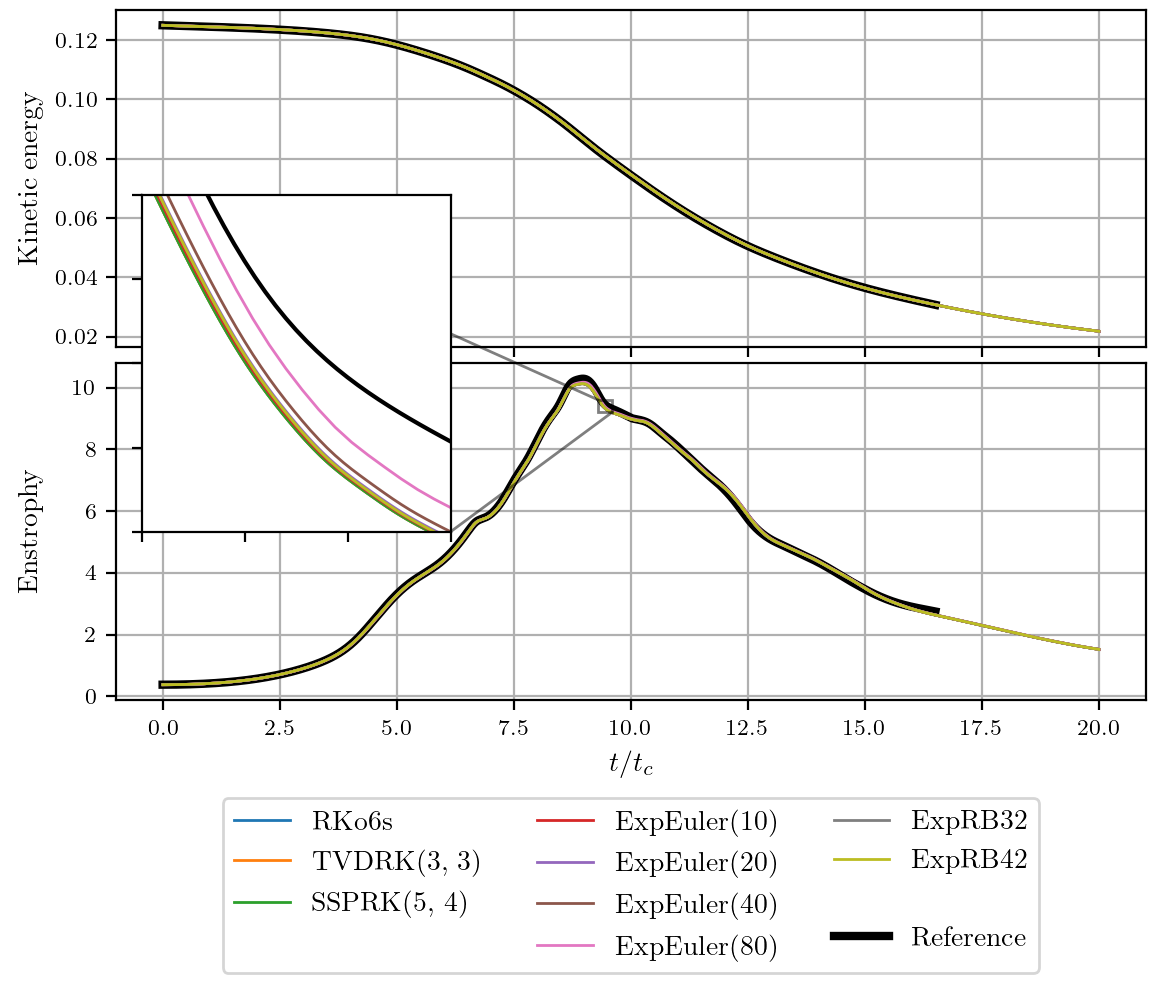
\includegraphics{figures/tgv_curves.png}
        \caption{Kinetic energy and enstrophy for various time integration methods compared to reference data.}
        \label{fig:tgv_curves}
      \end{figure}

      \begin{table}
        \center
        \begin{tabular}{c|cccc}
          Method       & $\mathcal{N}_\textrm{CFL}$ & $N_\textrm{iterations}$ & Time / iteration (s) & Total time (hh:mm:ss) \\ \hline
          RKo6s        & 0.28                       &                   50000 &                1.588 &             22:03:20  \\
          TVDRK(3, 3)  & 0.14                       &                  100000 &                0.833 &             23:08:20  \\
          SSPRK(5, 4)  & 0.28                       &                   50000 &                1.497 &             20:47:30  \\ \hline
          ExpEuler(10) & 1.4                        &                   10000 &                3.803 &             10:33:50  \\
          ExpEuler(20) & 2.8                        &                    5000 &                8.144 &             11:18:40  \\
          ExpEuler(40) & 5.6                        &                    2500 &               19.491 &             13:32:08  \\
          ExpEuler(80) & 11.2                       &                    1250 &               52.792 &             18:19:50  \\
          ExpRB32      & 2.8                        &                    5000 &               10.391 &             14:25:55  \\
          ExpRB42      & 2.8                        &                    5000 &               19.787 &             27:28:55  \\
        \end{tabular}
        \caption{
          Statistics for various time integration methods.
          Time corresponds to elapsed real time, or wall-clock time.
          A computation corresponds to the simulation of the Taylor--Green vortex from equation (\ref{eq:tgv}) on time interval $\left[0, 20 t_c\right]$.}\label{tab:tgv}
      \end{table}

      \paragraph{}
      Statistics for each time integration method are provided in table \ref{tab:tgv}.
      As the cost of the algorithms used in the time integration methods does not change between iterations, it makes sense to compute the average elapsed real time per iteration.
      Among the explicit methods, we see that the RKo6s and SSPRK(5, 4) methods run at a higher CFL number than the TVDRK(3, 3) method.
      However, they have more stages per iteration so each iteration takes longer, and the total elapsed real time is rather similar between all three methods.
      We note that the cost of one step of an explicit Runge--Kutta method is not proportional to the number of stages.
      Indeed, the implementation of the RKo6s method uses the fact that it is a low storage method to reduce the computational cost in terms of both time and memory.
      Nevertheless, the cost of an iteration of those explicit methods is much less than exponential methods.
      As expected, the cost of the exponential Rosenbrock--Euler method is similar to $d^2$ where $d$ is the dimension of the Krylov subspace used for the Arnoldi iteration \PS{vérifier ça}.
      As explained, the ExpRB32 method does not cost a lot more than the exponential Rosenbrock--Euler method that uses Krylov subspace with the same dimension.
      This is because the second stage uses only small Krylov subspace, and this is what is seen from the results in table \ref{tab:tgv}.
      We can draw two important conclusions from this analysis.
      First, we see that the exponential Rosenbrock methods are faster than the explicit Runge--Kutta methods available in JAGUAR.
      For some of them, they are almost twice as fast.
      Secondly, we see that the exponential Rosenbrock--Euler method can accurately simulate the Taylor--Green vortex at high CFL numbers.
      Accurate explicit methods would not work with such high CFL numbers, and even if implicit methods could they would not be accurate enough to capture and preserve the small scales of the flow.
      To reach high CFL numbers, we have to use larger Krylov subspaces, that make the method a lot slower.
      The method used here should not be used for actual applications: the goal was just to show feasibility.
      It seems that with exponential methods, the robustness can be increased by paying the price in terms of Krylov subspace dimension.
      We can think of ways to compute more accurately the $\varphi$-functions less expensively: by using restarted methods for instance, we can control the maximal dimension of the Krylov subspace.
      However this was not tried during this thesis.

      \paragraph{}
      This unsteady test case shows that exponential methods are interesting for our applications.
      We found a method that halves the elapsed real time, which is a great improvement for an unsteady simulation.
      We also showed that we could accurately simulate this flow while using high CFL numbers.
      It means that we have added more robust methods than the already existing ones.
      They could prove useful on applications where we are limited by the lack of stability of the explicit Runge--Kutta methods.


    \subsection{Industrial application: LS89}

      \PS{TODO}

      \paragraph{}
      We decided to try exponential methods on a last test case.
      Contrary to the previous two, we stepped out of the academic context with an industrial application.
      It is a simulation of the flow inside the LS89 turbine blade cascade that was studied experimentally by the von Karman Institute \cite{ArtsLambertdeRouvroit1992}.
      We choose this test case as it has already been done with several solvers, including JAGUAR recently \cite{BrunetCronerMinotEtAl2018}.
      We use a two-dimensional unstructured mesh, made of \num{2374} cells, that was extruded over 20 cells for a length of $0.15 c$ with $c$ the chord of the turbine blade.
      The final three-dimensional mesh made of \num{47480} cells is shown in figure \ref{fig:ls89_mesh}.
      The mesh is periodic in the extruded direction and the vertical direction.
      The boundary condition at the wall is isothermal, with $T_\textrm{wall} = 297.75 \si{\kelvin}$.
      At inlet, the stagnation conditions are $P_0 = \num{184900}\si{\pascal}$ and $T_0 = 409.2\si{\kelvin}$.
      We set the pressure at outlet at $P = \num{116487}\si{\pascal}$.


      \begin{figure}
        \centering
        % 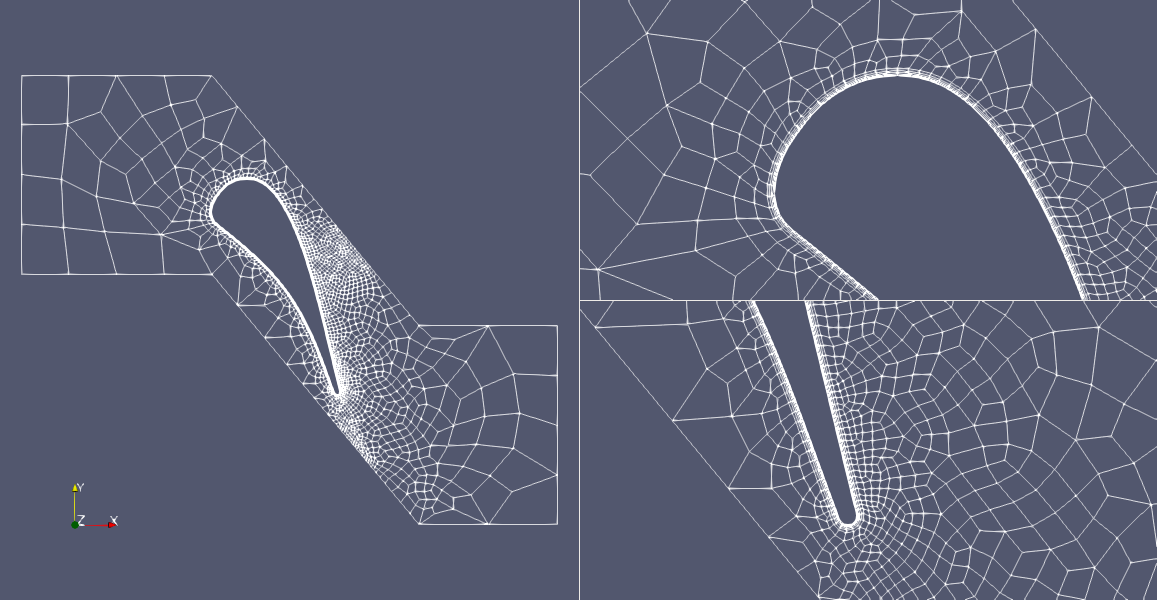
\includegraphics{figures/ls89_mesh.png}
        \caption{\PS{TODO}}
        \label{fig:ls89_mesh}
      \end{figure}


\part*{Appendices}
\addcontentsline{toc}{part}{Appendices}
\appendix

  \chapter{Conservative preconditioning}
  \label{appendix:conservative_preconditioning}

    \paragraph{}
    Let us consider the ordinary differential equation:
    \begin{equation}
      M \frac{\mathrm{d}Q}{\mathrm{d} t} = \operatorname{F}\left(Q\left(t\right)\right) .
    \end{equation}
    This equation comes from the Finite Volume discretisation, where $Q$ is the vector of the conservative variables and $\operatorname{F}$ a conservative right-hand side.
    To keep this simple, we consider that there is a single conservative variable, so that the dimension of $Q$ is equal to the number of cells.
    This is only to simplify the notations, but everything can be adapted to use more conservative variables.
    The mass matrix $M$ is a diagonal matrix where the $i$th diagonal coefficient corresponds to the volume of the $i$th cell.
    We note by $S$ the vector of the same dimension as $Q$ made of ones and transposed.
    This way, multiplying on the left a vector by $S$ amount to sum a vector components.
    The conservation property of the equation means that $S \operatorname{F}\left(Q\right) = 0$ or equivalently that the sum of the conservative variable over the domain $SMQ$ is constant.

    \paragraph{}
    When solving this equation with the explicit Euler method, we have at the $n$th step that:
    \begin{equation}
      M\delta Q_n = \Delta t \operatorname{F}\left(Q_n\right)
    \end{equation}
    with $\delta Q_n = Q_{n+1} - Q_n$.
    Is is clear that $SMQ_{n+1} = SMQ_n$, and so the explicit Euler method preserves the conservation property.

    \paragraph{}
    When using the implicit Euler method with a single linearisation, we need the Jacobian matrix $J_n$ of the function $\operatorname{F}$ evaluated in $Q_n$.
    Since $J_n = \operatorname{F}'\left(Q_n\right)$ and $S\operatorname{F}\left(Q_n\right) = 0$, we have $SJ_n = 0$ also.
    The method gives the increment $\delta Q_n$ as the solution of:
    \begin{equation}
      \left(M - \Delta t J_n\right) \delta Q_n = \Delta t \operatorname{F}\left(Q_n\right) .
    \end{equation}
    Multiplying this relation on the left by $S$ and using that $SJ_n = S\operatorname{F}\left(Q_n\right) = 0$, we have $SM\delta Q_n = 0$, which means this method also preserves the conservation property.

    \paragraph{}
    However, we do not usually use the exact solution of the linear problem but the solution of a subspace Krylov method.
    Let us consider that we use $k$ steps of a Krylov subspace method with a zero initial guess.
    Then, the increment belongs to the corresponding Krylov subspace:
    \begin{equation}
      \delta Q_n \in \operatorname{Vect}\left( \left(M - \Delta t J_n\right)^i \operatorname{F}\left(Q_n\right) \right)_{0\leq i < k} .
    \end{equation}
    Now, there are no reasons for $SM\delta Q_n$ to be equal to zero.
    For example, the solution computed with the smallest Krylov subspace dimension ($k = 1$) is parallel to $\operatorname{F}\left(Q_n\right)$, and then $SM\delta Q_n \propto SM\operatorname{F}\left(Q_n\right)$ and therefore is not null.

    \paragraph{}
    With preconditioning however, we can recover the conservation property.
    If we use the invert of the mass matrix as a preconditioner, either a left or a right one, we have that:
    \begin{equation}
      \delta Q_n \in \operatorname{Vect}\left(v_i\right)_{0\leq i < k} \quad\textrm{with}\quad v_i = \left(\operatorname{Id} - \Delta t M^{-1} J_n \right)^i M^{-1} \operatorname{F}\left(Q_n\right) .
    \end{equation}
    We can verify by recurrence that $SMv_i = 0$:
    \begin{itemize}
      \item $SMv_0 = SMM^{-1}\operatorname{F}\left(Q_n\right) = S\operatorname{F}\left(Q_n\right) = 0$
      \item if $SMv_i = 0$, then $SMv_{i+1} = SM \left(\operatorname{Id} - \Delta t M^{-1} J_n \right) v_i = SMv_i - \Delta t S J_n v_i = 0$ as $SJ_n = 0$.
    \end{itemize}
    Then, we have that $SM\delta Q_n = 0$ which means the preconditionned method preserves the conservation property.


\bibliography{bibliography.bib}
\bibliographystyle{ieeetr}
\addcontentsline{toc}{chapter}{Bibliographie}

\end{document}
